


\documentclass[12pt]{article}
\usepackage{natbib}
\usepackage[flushleft]{threeparttable}
\usepackage{longtable}
\usepackage{bm}

\usepackage{caption}

\usepackage[toc,page,header]{appendix}

\usepackage{listings}
\usepackage[english]{babel}
\usepackage[utf8]{inputenc}
\usepackage[dvips]{graphicx}
\usepackage{amsmath,amsthm,amssymb,tipa,dsfont,mathtools,mathrsfs,here,titlesec,fancyhdr}
\usepackage{anysize}
\usepackage{subfigure}
\usepackage{color}
\usepackage{enumerate}
\usepackage{booktabs}
\usepackage{rotating}
\usepackage{parskip} % to avoid // 
\usepackage[hidelinks]{hyperref}
\usepackage{url}
\usepackage{multirow}
\renewcommand{\qedsymbol}{\rule{0.7em}{0.7em}}
\usepackage{comment} % begin{comment} to comment large sections
\usepackage[font=scriptsize]{caption}
\usepackage{rotating} % to rotate tables 
\usepackage{tikz}
\usetikzlibrary{shapes,decorations,arrows,calc,arrows.meta,fit,positioning}
\tikzset{
	-Latex,auto,node distance =1 cm and 1 cm,semithick,
	state/.style ={ellipse, draw, minimum width = 0.7 cm},
	point/.style = {circle, draw, inner sep=0.04cm,fill,node contents={}},
	bidirected/.style={Latex-Latex,dashed},
	el/.style = {inner sep=2pt, align=left, sloped}
}

\definecolor{Grey}{RGB}{150, 150, 150}
\definecolor{PPblue}{RGB}{0,114,198}
\definecolor{VOXblue}{RGB}{0,114,198}
\definecolor{PSOEred}{RGB}{232,0,0}
\definecolor{UPred}{RGB}{232,0,0}
\newcommand{\sym}[1]{\rlap{#1}}

\definecolor{mypink}{rgb}{0.858, 0.188, 0.478}
\definecolor{myorange}{rgb}{1.0, 0.49, 0.0}
\definecolor{mypurple}{rgb}{0.6, 0.4, 0.8}
%\usepackage[colorlinks=true,linkcolor=blue,citecolor=blue,hyperfootnotes=false]{hyperref} 
\hypersetup{
	colorlinks,
	citecolor=blue,
	linkcolor=mypink,
	urlcolor=mypurple}
%Els comandaments següents són per a linkejar (han d'estar al final de tots els usepackage)
%\usepackage[colorlinks]{hyperref}%aquests paquets s'utilitzen per a poder linkejar coses.
%\hypersetup{citecolor=red}
%\hypersetup{linkcolor=red}
%\hypersetup{urlcolor=red}
%\usepackage{cleveref}%aquest també.

\usepackage[T1]{fontenc} % for porper quotation marks 
\PassOptionsToPackage{svgnames}{xcolor}
\usepackage{pgfplots}


\usepackage{tcolorbox}
\usepackage{lipsum}
\tcbuselibrary{skins,breakable}
\usetikzlibrary{shadings,shadows}
\newenvironment{myblock}[1]{%
	\tcolorbox[beamer,%
	noparskip,breakable,
	colback=LightBlue,colframe=DarkBlue,%
	colbacklower=DarkBlue!75!LightBlue,%
	title=#1]}%
{\endtcolorbox}

\usepackage{tikz}
\usetikzlibrary{shapes,decorations,arrows,calc,arrows.meta,fit,positioning}
\tikzset{
	-Latex,auto,node distance =1 cm and 1 cm,semithick,
	state/.style ={ellipse, draw, minimum width = 0.7 cm},
	point/.style = {circle, draw, inner sep=0.04cm,fill,node contents={}},
	bidirected/.style={Latex-Latex,dashed},
	el/.style = {inner sep=2pt, align=left, sloped}
}














\renewcommand{\baselinestretch}{1.2} %separació entre linies
\marginsize{2.3cm}{2.3cm}{1cm}{2cm} %Margens


%ací definim els colors que anem a gastar
\definecolor{secction}{rgb}{0.62,0.31,0.00}
\definecolor{subsection}{rgb}{0.33,0.00,0.33}
\definecolor{mygreen}{RGB}{28,172,0}


%S'utilitza per a insertar programes de forma més professional
%\lstset{language=Matlab,numbers=left,frame=single,title=\lstname}
\lstset{language=Matlab,%
    %basicstyle=\color{red},
    breaklines=true,%
    morekeywords={matlab2tikz},
    keywordstyle=\color{blue},%
    morekeywords=[2]{1}, keywordstyle=[2]{\color{black}},
    identifierstyle=\color{black},%
    %stringstyle=\color{mylilas},
    commentstyle=\color{mygreen},%
    showstringspaces=false,%without this there will be a symbol in the places where there is a space
    numbers=left,%
    numberstyle={\tiny \color{black}},% size of the numbers
    numbersep=9pt, % this defines how far the numbers are from the text
    emph=[1]{for,end,break},emphstyle=[1]\color{blue}, %some words to emphasise
    %emph=[2]{word1,word2}, emphstyle=[2]{style},
}

\usepackage[colorinlistoftodos,textwidth=3cm]{todonotes}
\newcommand{\todoINFO}[1]{\todo[color=blue!25]{INFO: #1}}
\newcommand{\todoIMPORTANT}[1]{\todo[color=red!25]{IMPORTANT: #1}}
\newcommand{\todoREV}[1]{\todo[color=green!25]{REVIEWED: #1}}
%Aquí redefinimos los comandos teorema, nota, etc... para que sea más fácil de escribir. Lo que está entre corchetes "[,]" es para que enumere los teoremas en función de la sección, si se quita, lo enumera sobre el total.
\theoremstyle{plain}
\newtheorem{teo}{Theorem}[section]
\newtheorem{prop}{Proposition}[section]
\newtheorem{exe}{Exercise}
\theoremstyle{definition}
\newtheorem{defi}{Definition}[section]
\newtheorem{nota}{Note}
\DeclarePairedDelimiter\abs{\lvert}{\rvert}%
\DeclarePairedDelimiter\norm{\lVert}{\rVert}%
%abreviatures dels comandaments "begin/end". Es una chorradita por no escribirlo todo, puedes usarlo o no.
\newcommand{\be}{\begin{exe}}
\newcommand{\ee}{\end{exe}}
\newcommand{\bt}{\begin{teo}}
\newcommand{\et}{\end{teo}}
\newcommand{\bd}{\begin{defi}}
\newcommand{\ed}{\end{defi}}
\newcommand{\bn}{\begin{nota}}
\newcommand{\en}{\end{nota}}
\newcommand{\bp}{\begin{proof}}
\newcommand{\ep}{\end{proof}}
\usepackage{accents}
\newcommand{\ubar}[1]{\underaccent{\bar}{#1}}

%abreviatures de símbols. Esto en realidad no lo utilizo nunca, pero si te acostumbras es más cómodo.
\newcommand{\e}{\exists}
\newcommand{\fa}{\forall}
%\newcommand{\iff}{\Leftrightarrow}

%Comandaments utilitzats per a donar un millor estil a les pàgines (la xorradeta de la linia de dalt)
\usepackage{fancyhdr}
\pagestyle{fancy}
\lhead{}
%\rhead{Luis Ignacio Menéndez García}
%\renewcommand{\footrulewidth}{0.3pt}

\renewcommand{\headrulewidth}{0pt}   % no line under the header
\renewcommand{\footrulewidth}{0pt}   % no line above the footer


%here we use a new command for the figures titles
\newcommand*{\figuretitle}[1]{%
	{\centering%   <--------  will only affect the title because of the grouping (by the
		\textbf{#1}%              braces before \centering and behind \medskip). If you remove
		\par\medskip}%            these braces the whole body of a {figure} env will be centered.
}

\DeclareMathOperator*{\E}{\mathbb{E}}
\DeclareMathOperator*{\R}{\mathbb{R}}
\DeclareMathOperator*{\Lag}{\mathscr{L}}
\DeclareMathOperator*{\contr}{\Rightarrow\Leftarrow}
\DeclareMathOperator*{\convprob}{\overset{p}{\to}}
\DeclareMathOperator*{\convas}{\overset{a.s.}{\to}}
\DeclareMathOperator*{\convd}{\overset{d}{\to}}
\DeclareMathOperator*{\impose}{\stackrel{!}{=}}



%change colorlinks=false if you don't wan't any hyperlinks to have color

%cmd+n to open a new wnvironment for equation see macros in options of texstudio


% in pack.tex  ────────────────────────────────────────────────
\usepackage{titlesec}



\usepackage{minitoc}          % ← load minitoc *after* titlesec

% ------------------------------------------
% leave \thepart numeric; just hide the label text
\renewcommand\thepart{}      % ← KEEP THIS COMMENTED OUT
\renewcommand\partname{}      % ok to suppress the printed “Part”


%\renewcommand{\part}[1]{\addcontentsline{toc}{part}{#1}}













\captionsetup[figure]{font=normalsize, labelfont=bf}

%\usepackage{chngcntr}   % lets you reset & prefix counters cleanly








%\usepackage[paperwidth=275.9mm, paperheight=279.4mm]{geometry} 
\usepackage{afterpage}
\usepackage{calligra}
\newcommand{\share}{\mbox{\calligra{S}}}

\title{The Impact of Political Campaigns on Demand for Partisan News}
\author{Luis  Menéndez \thanks{Universitat Autònoma de Barcelona, CSIC and Barcelona School of Economics.}} %omit the footnote and thanks if needed
\date{%
	\today\\[2ex]
	{\bfseries Job Market Paper}\\[1ex]
	{\normalsize\href{https://www.dropbox.com/scl/fi/f3546vufz11vj5r63xml4/elections_draft.pdf?rlkey=exjw9vm3sasahlb54ohjf2tyx\&e=1\&dl=0}{Latest version here}}
}

\begin{document}
	
\renewcommand\thepart{}      % ← KEEP THIS COMMENTED OUT
\renewcommand\partname{}      % ok to suppress the printed “Part”
	
	
	\maketitle
	
	\begin{abstract}
		

	
		Political polarization in news consumption has recently gained attention, yet policies to limit it are hard to evaluate. This paper introduces a novel, self-collected dataset on Spanish prime-time TV news. I identify stories minute-by-minute and match them across newscasts to compare editorial treatment. Combining machine-learning methods with large language models, I classify the partisan slant of each story and use the resulting data to document changes in news coverage during the 2023 presidential campaign. I then match these data to high-frequency audience-meter records and estimate a random-coefficients demand model, using shifts in the daily wire-service story mix as instruments for slant. I find significant evidence of affective polarization only after the election campaign begins. Given the demand estimates, I back out outlets’ content preferences from a horizontal-differentiation game. Finally, I run counterfactual simulations to assess the effect of policies regulating campaign airtime. My framework offers a tractable tool for evaluating media policies aimed at content fairness or fighting misinformation.
		
		
		
	\end{abstract}
	
	


		\doparttoc % Tell to minitoc to generate a toc for the parts
	\faketableofcontents % Run a fake tableofcontents command for the partocs
		\part{} % Start the document part
		
%	\parttoc
	
	\clearpage
	

	
	

	%\parttoc % Insert the document TOC
	

	
	
	\section{Introduction}
	
	
	
	
%	https://cepr.org/voxeu/blogs-and-reviews/rethinking-media-pluralism-france

Political polarization has surged in both the United States and Europe over the past decade \citep{ Reiljan2019FearAL}. Extensive research highlights the role of social media in driving this trend \citep{Zhuravskaya2020}. However, \cite{Boxell2020CrossCountryTI}  find that polarization in the US has increased the most  precisely among groups that re more likely to consume traditional, rather than social media. Still nowadays television remains the primary source of political information across Europe and it is known to have large effects on voting outcomes \citep{dellavigna2007fox, gentzkow_turnout, martin2017}, education \citep{gentzkow2008preschool} and culture \citep{jensen2009power}. The mechanisms through which this influence operates—specifically, the preferences driving viewer demand—remain understudied.

In response, regulators have tightened rules in media markets, but designing and evaluating effective policies remains challenging. The first obstacle is measurement: developing indicators of partisan slant that are both scalable to thousands of hours of content and comparable across outlets is inherently difficult. Second, even with good measures, there is a fundamental identification problem. Market equilibrium introduces endogeneity: the content an outlet provides is a strategic response to viewer preferences, while viewers choose outlets that align with their views. This feedback loop makes it difficult to separate viewer demand from the editorial decisions of the channels.

This paper proposes a novel methodology to address these two challenges. I estimate the extent of confirmation bias and polarization in the demand for political content and examine how these dynamics evolve during electoral campaigns in Spain, the most polarized country in Europe \citep{edelman_trust_2023}.

To tackle the measurement challenge, I construct a unique dataset that integrates the supply and demand of political content in Spanish TV news. On the demand side, high-frequency audience-meter data address well-known limitations of survey-based studies \citep{prior}. On the supply side, I compile a text corpus of all news segments and employ Large Language Models (LLMs) and machine learning to classify their political tone. This approach provides a granular, daily measure of the airtime and tone allocated to each political party. I further show how my stance measure compares with previous text methods based on congress speeches, dictionary counts, and image appearances of political leaders.

To overcome the identification problem, I propose a strategy that leverages exogenous shocks to the daily news supply. I collect all stories from the largest news aggregator that supplies these outlets, using it as a proxy for the day’s available news landscape. While outlets aim to maintain their long-term ideological positions, these daily news shocks constrain their broadcasts, making some days exogenously more favorable to one ideological side. Descriptive evidence supports this mechanism: right-wing (left-wing) channels expand coverage when the pool of favorable right-wing (left-wing) stories is larger.

My findings align with prior evidence on polarized news consumption in the United States \citep{Peterson2017Echo}. Outside of campaign periods, there is no systematic asymmetry in political-content demand between right- and left-leaning audiences; viewers generally prefer negative political tone. During campaigns, however, affective polarization emerges: right-leaning viewers increasingly seek negative coverage of the left and more positive coverage of the right, with a mirror pattern among left-leaning viewers.

Using these demand estimates, I model and estimate news production. Outlets engage in a differentiation game, choosing daily slant to maximize viewership. Production costs depend on the mix of stories available each day. Identification relies on timing: I exploit variation in news stories between midday and evening broadcasts to estimate outlets’ slant production costs. Producing left-favoring content is costly for all channels, particularly for right-leaning ones, while right-favoring content generally increases payoffs, though less so for left-leaning outlets.

Existing media regulations to fight political plurality have often been found to be insufficient due to poor measurement and, consequently, lack of enforcement \citep{cage_assemblee}. I run a counterfactual in which Spain adopts a policy already used in several European countries: proportional airtime during election campaigns. I estimate the equilibrium of the game forcing outlets to devote relative political time to a party according to past election results. Consistent with the way this policy is enforced, I only regulate total airtime, thus letting channels adjust through tone.

This paper is the first existing effort to quantitatively monitor media in Spain and contributes to the debate on regulation in media markets.



\textbf{Related Literature}


This paper contributes to several strands of the media and political-economics literature. Existing work has measured media bias through candidate endorsements \citep{ChiangKnight2011}, text-based slant \citep{gentzkow2010media,GentzkowShapiroTaddy2019}, and screen-time shares \citep{durante2012partisan,CageHengelHerveUrvoy2022}. I propose a new methodology that combines ideological tone and airtime using large language models (LLMs), allowing for a high-frequency, scalable slant measure. This approach improves on prior text-based classifications by validating against survey-based preferences and tracking tone and exposure at the story level. The result unifies previously separate approaches \citep{puglisi_review}, and by incorporating variation in the news supply chain, connects to work on bias driven by \emph{filtering} versus \emph{distortion} \citep{gentzkow2014media}.


On the demand side, I build on recent work estimating preferences for like-minded news \citep{SimonovRao2022,gentzkow2010media}. Unlike \cite{SimonovRao2022}, who treat the supply side as fixed and recover audiences’ tastes from random day-to-day swings in the overall share of government-sensitive stories, I  rely on product-level cost shifters that move each station’s slant differently within the same day. 


Past works have found significant heterogeneity in content consumption by demographic groups, as documented by \citet{gambaro2021revealed} for Italian TV markets and for US media markets \citep{bang2023, BangSieg2025}. I focus on ideological taste differences and contribute to the literature on media-driven polarization. While experimental evidence points to limited persuasion due to self-selection \citep{arceneaux_johnson_2013}, and reinforcement effects among partisans \citep{levendusky}, \citet{martin2017} show that cable-news polarization can account for much of the rise in voter polarization: using channel positions as instruments for U.S. TV consumption,. Although data limitations prevent me from modeling belief updating directly as in their work, I present correlational evidence linking media and political polarization.

Methodologically, the paper contributes to work that uses text embeddedings  and imagery to construct product characteristics in demand models \citep{compiani2025demandestimationtextimage}. I introduce a scalable index of media slant that incorporates both tone and intensity of coverage and compare it to slant measures based on facial recognition. This tool enables to account for differentiation in products that might otherwise seem homogeneous such as TV news. 

However, this richer product space raises standard concerns about endogeneity. I address this with a novel identification strategy that exploits supply shocks in news content drawn from upstream aggregators,\footnote{ A similar mechanism appears in \citet{milena}, who study how an Associated Press keyword ban altered U.S. newspaper coverage} extending instrument designs based on demographic changes over pricing zones \citep{fan,gentzkow2010media} or candidate positions across electoral precincts \citep{longuet-marx2025party}.


Finally, prior research evaluates policy interventions in television markets—bundling \citep{crawford_yurukoglu}, vertical integration \citep{crawford_vertical}, ownership changes \citep{MARTIN_McCRAIN_2019,CageHengelHerveUrvoy2022}, and entry \citep{prat_stromberg_entry}. I extend this literature by assessing content regulations aimed at enhancing political plurality.

\begin{comment}

This paper contributes to several strands of the media- and political-economics literature. Earlier studies measure media bias using candidate endorsements \citep{ChiangKnight2011}, textual analysis \citep{gentzkow2010media,GentzkowShapiroTaddy2019}, or the share of speaking time allocated to each side \citep{durante2012partisan,CageHengelHerveUrvoy2022}. I introduce a new methodology that merges slant and airtime by employing large language models (LLMs) for text classification. Validation with survey data on political preferences shows that this approach outperforms previous text-based methods that rely on congressional speeches. In addition, the machine-learning framework pinpoints both the tone and the time devoted to the same story on a given day across outlets, allowing me to track the topics on which outlets converge. The measure thus unifies several approaches previously treated separately in the literature \citep{puglisi_review} and complements theoretical work on the sources of media bias. By using upstream news providers as proxies for the overall news landscape, the analysis also speaks to and could be integrated in future works to study bias generated by \emph{filtering} versus outright \emph{distortion} \citep{gentzkow2014media}

The closest empirical work estimates demand for like-minded political news. \citet{SimonovRao2022} classify government-sensitive content and match it to individual browsing data to estimate a structural model of news acquisition; they find that outlet-specific factors drive demand and create inertia in sensitive-news consumption. Other studies document sizable demographic differences in news choices across content types \citep{gambaro2021revealed,bang2023}.

Evidence on the media’s role in political polarization is mixed. Laboratory experiments suggest that already-polarized viewers self-select into polarized news sources, with media having limited effects \citep{arceneaux_johnson_2013}, but there is evidence of polarizing effects by affecting those already away from the political center \citep{levendusky}. \citet{martin2017} show that cable-news polarization can account for much of the rise in voter polarization: using channel positions as instruments for U.S. TV consumption, they estimate a dynamic model in which ideology evolves with the slant consumed and conclude that roughly two-thirds of the observed increase stems from cable news. I introduce a new identification strategy that isolates short-run effects in settings where their instrument is infeasible. Although data limitations prevent me from modeling belief updating directly, I present correlational evidence linking media and political polarization: regions with more polarized media consumption are also more politically polarized, and the latter series exhibits a clear break during campaign periods.


Social media is known to amplify polarization by creating online echo chambers \citep{bail2018exposure,Zhuravskaya2020}. I add to newer evidence on traditional media \citep{schneider2025media} by showing that television can likewise intensify polarization during election campaigns—a critical period for voting decisions.


Recent studies incorporate text embeddings and imagery to build product characteristics in demand models \citep{compiani2025demandestimationtextimage}. I propose a scalable method for constructing slant characteristics from text that captures both coverage intensity and ideological tone, offering a market-differentiation index for products that might otherwise appear homogeneous. 

However, although the increase in product characteristics helps building variations cross products, this poses the risk of endogeneity in some of these attributes. Previous works instrumented endogenous characteristics with excluded shifters for firm mark ups exploiting demographics over pricing zones \citep{fan,gentzkow2010media}; and candidate positions over precinct levels \citep{longuet-marx2025party}. This work offers a new identification strategy based on cost shifters on content production exploiting supply-chain flows from news aggregators \footnote{ A similar mechanism appears in \citet{milena}, who study how an Associated Press keyword ban altered U.S. newspaper coverage}. 

Finally, prior research evaluates policy interventions in television markets—bundling \citep{crawford_yurukoglu}, vertical integration \citep{crawford_vertical}, ownership changes \citep{MARTIN_McCRAIN_2019,CageHengelHerveUrvoy2022}, and entry \citep{prat_stromberg_entry}. I extend this literature by assessing content regulations aimed at enhancing political plurality.


\end{comment}

\textbf{Rest of the paper}

The rest of the paper is organized as follows. In Section \ref{section:context}, I briefly summarize the Spanish political and TV landscape. Section \ref{section:data} introduces the data and describes the text analysis techniques I employ, along with descriptive statistics on both the content and audience sides. In Section \ref{section:market}, I first describe the market setup and the demand model and then discuss the endogeneity problem and the instrumental-variables approach. Results from the demand estimation are shown in Section \ref{section:results}. Finally, Section \ref{sec:supply} presents the identification and estimation of the supply-side parameters.

	
	
	\section{Context}
	
	Before detailing the data used and the text classification methodology, I provide a brief context on the Spanish TV market. To compare the use of TV versus other media for political information, I provide descriptive evidence based on survey data for both Spain and Europe. Finally, I describe the political context in Spain by introducing the main parties considered in the analysis and the changes in party structure leading to the general elections of 2023.
	
	\label{section:context}
	
	\subsection*{Spanish TV market}
	
	The Spanish TV market is a competitive mix of public and private broadcasters, with Televisión Española (TVE) positioned as the state-owned provider of news, cultural programs, and entertainment. The two primary private conglomerates, Atresmedia and Mediaset, dominate the market. Atresmedia operates Antena 3 and LaSexta, while Mediaset controls Telecinco. Altogether, their evening TV news editions (the product analyzed in this paper) capture around $50\%$ of the market share, equating to 4.5 million viewers, which represents $10\%$ of the Spanish population. For comparison, the average number of viewers for the most popular news program in the U.S., Fox News, is around 2.2 million.
	
	\subsection*{Traditional media and political information}
	
	Traditional media remain the primary source of information in most European countries \citep{europarl2024}. Figure \ref{fig:motivation} shows the main media used to acquire political information in Spain by age group, as reported by the 2023 survey from the Centro de Investigaciones Sociológicas (CIS) under the question: \textit{"Through which media do you usually get information about news in Spain?"}. Traditional media are represented in the left panel as radio, press, and television. Television remains the dominant source of political information for those aged 50 and older and dominates social media for all but the youngest cohort. This pattern, however, is not specific to Spain. Figure \ref{fig:motivation2} shows that television remains the dominant source of political information in Europe, particularly among older age groups. While younger cohorts (15--24, 25--39) rely more on social media, TV consistently outweighs social media among those aged 40 and above, with the gap widening significantly in the 55+ age group. This pattern highlights television’s enduring influence in European media landscapes, especially for older demographics, despite the rise of digital platforms.
	

	\begin{figure}[h!]
		\centering
		\caption{Top media source to acquire political information by age cohorts in Spain}
		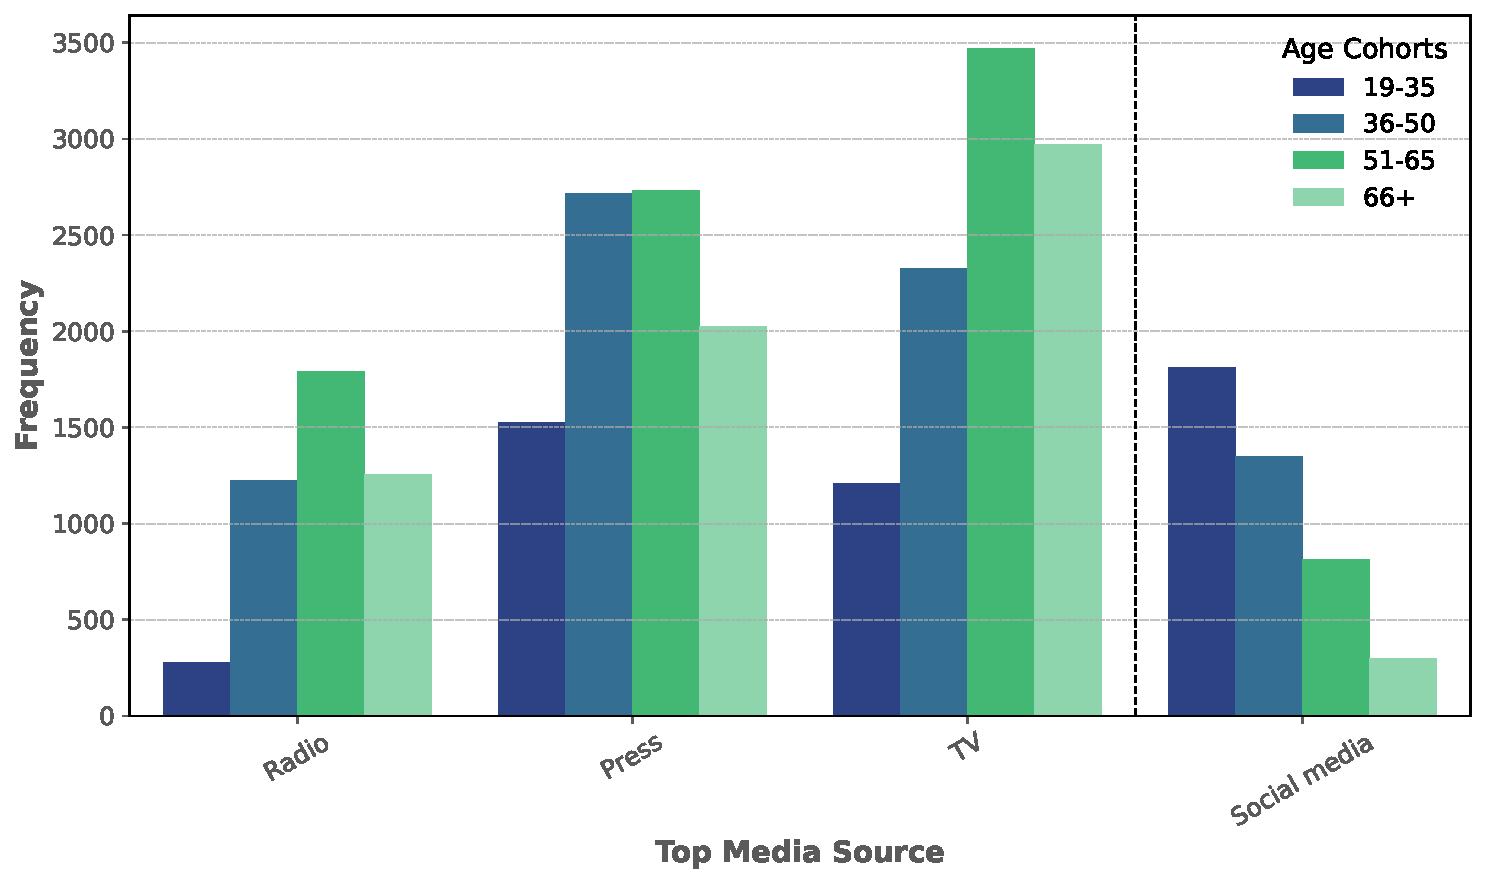
\includegraphics[width=120mm]{figures/age_cohorts}
\caption*{\small Notes: Histogram on the preferred media used for political information in Spain.  
	Source: Barómetro CIS, 2023. }
\label{fig:motivation}
	\end{figure}
	
	

	
	
	\subsection*{Political Context}
	
	Political power in Spain has historically been dominated by a two-party system, with either the Socialist Party (PSOE) or the Conservative Party (PP) in power. The emergence of the left-wing party Podemos (UP) following the 15M movement marked a significant shift, as the party began to attract a substantial portion of the electorate.\footnote{Relevant for this period of study is the integration of Podemos into the new political party SUMAR. All classification metrics account for this transition, but throughout the text, I refer to UP as either Podemos or SUMAR after its creation.} Of particular interest is the rise of the far-right party VOX, which made notable gains in the regional elections held on May 28, 2023, raising the possibility of forming a coalition with the Popular Party (PP). In response, the day after the regional elections, President Pedro Sánchez decided to bring forward the general elections to June 23, 2023.\footnote{I refer readers to the \href{https://luisignaciomenendez.github.io/media_monitor/index.html}{Spanish Media Monitor} webpage to explore various metrics of coverage across political parties and actors.} For the rest of the analysis, parties will be pooled into right (PP and VOX) and left (PSOE and Podemos).
	
	\section{Data and Descriptive Statistics}
	\label{section:data}
	
	I build a unique dataset that captures both the demand and supply sides of TV news in the Spanish market. For the demand side, I use minute-by-minute viewership data for the four main channels that offer daily TV news programs: TVE, Antena 3, LaSexta, and Telecinco. On the content side, I build a scraping pipeline that records the daily news programs live and processes this information into text. This dataset spans from December 2022 to July 2023 on a daily basis. It is complemented by all the stories published in Spanish by the largest news provider. Finally, I make use of survey and weather data as controls.
	
	\textbf{Audience Data}
	
	I use Audimeter, a high-frequency audience data source provided by Kantar Media, to observe the share of viewers for each channel at each day and minute. Although I do not have individual-level data on choices, I have geographical disaggregation for the 16 autonomous regions in Spain (also referred to as regions hereinafter), which I match to survey demographics\footnote{The Canary Islands and La Rioja are excluded due to different time zones and zero market shares; respectively. Similarly, peak days with sport events that altered the news schedule were also removed.}. The shares are specific to the evening TV news shows, which, with the exception of LaSexta at 20:00, start at 21:00 daily. For this analysis, this channel’s program is treated as if it occurred simultaneously with the others.\footnote{This might pose problems in the substitutions toward the outside option and specifically with  \textit{connected substitutes} assumption in \cite{gandhi2019measuring}.  }
	
	\textbf{TV Content}
	
	I record daily TV news videos and use Google Cloud infrastructure to store and process the data. Videos are converted to audio, and I use machine learning (\textit{speech-to-text}) to obtain text transcripts. Although visuals are not used in the main estimation due to computational constraints, I show comparisons between image and text metrics below. A more detailed explanation of the entire downloading pipeline can be seen in Appendix Figure \ref{fig:pipeline}.
	
	I consider both the evening and midday editions of TV news programs. This product offers a unique environment to test substitutability for several reasons. First, even though channels offer other political programs, the homogeneity of TV news allows for very clean comparisons. These programs are broadcast every day at almost the same time and all share a very similar structure, with a presenter introducing the main stories of the day. The fact that the structure is so similar makes them almost perfect substitutes and the key differentiation (aside from vertical, quality components) is therefore the way they present the information. Third, TV news is highly fact-checked and remains the most trusted source of information in Spain.\footnote{The Digital News Report 2023 reveals notable patterns in public trust towards news media across Europe, with Spain reflecting a stable but modest level of confidence. According to the report, the public service broadcaster RTVE and Antena 3 Noticias continue to rank as the most trusted news sources, with trust levels of 53\% and 52\%, respectively. LaSexta registers a trust increase of 2.7 percentage points over the previous year, reaching approximately 47\%, and Telecinco follows at 39\% \citep{reuters_dnr_2023}.}
	
	\textbf{Agencia EFE}
	
	I obtain all news stories provided in Spanish by one of the largest news agencies in the world, Agencia EFE. Similar to Reuters or AP, this agency mainly sells content and images to third-party newscasts. I document that all the outlets in my sample are clients of Agencia EFE.\footnote{See, e.g., collaborations with \href{https://www.telecinco.es/autores/agencia-efe/}{Mediaset}, \href{https://cadenaser.com/nacional/2024/09/22/el-teletexto-una-herramienta-olvidada-que-aun-perdura-en-nuestras-televisiones-cadena-ser/}{Atresmedia}, and \href{https://www.rtve.es/rtve/20130301/rtve-agencia-efe-firman-convenio-colaboracion/611440.shtml}{RTVE}.} I have information on the title of each story along with a short summary segment. There are around 41K stories for my sample period.
	
	\textbf{Survey Data}
	
	To understand polarization behavior, I use survey data gathered from the Centro de Investigaciones Sociológicas (CIS). Specifically, I rely on the "intention to vote" question and map it onto my binary left–right spectrum according to the parties described above. This data is monthly and cross-sectional.
	
	\textbf{Weather}
	
	I use meteorological data on daily rainfall per region for the time span matching the TV news programs (18:00–00:00) from the Spanish Meteorological Agency (AEMET).
	
	\subsection{Political Coverage and Elections}
	
	I divide the time span into two periods. The \textit{off-campaign} period starts at the beginning of data collection in December 2022 and extends to the start of the first publicly announced political campaign on May 13, 2023. The \textit{campaign} period covers both regional and general election campaigns and lasts until July 17, 2023, the day of the general elections.
	
	Figure \ref{fig:coverage} shows the weekly average proportion of time devoted to national politics over time, where the \textit{campaign} period corresponds to the shaded span and vertical dashed lines mark the beginning of the campaign, the regional elections, and the national elections, respectively. A channel is defined to spend one minute on national politics if the associated text for that minute contains any of the party matches in the dictionaries in Table \ref{table:politics}. Off-campaign, channels spend on average nearly 18\% of their daily time on politics. Naturally, this increases to 30\% during campaign periods.
	
	
	\begin{figure}[h!]
		\caption{Proportion of time devoted to politics over time}
		\centering
		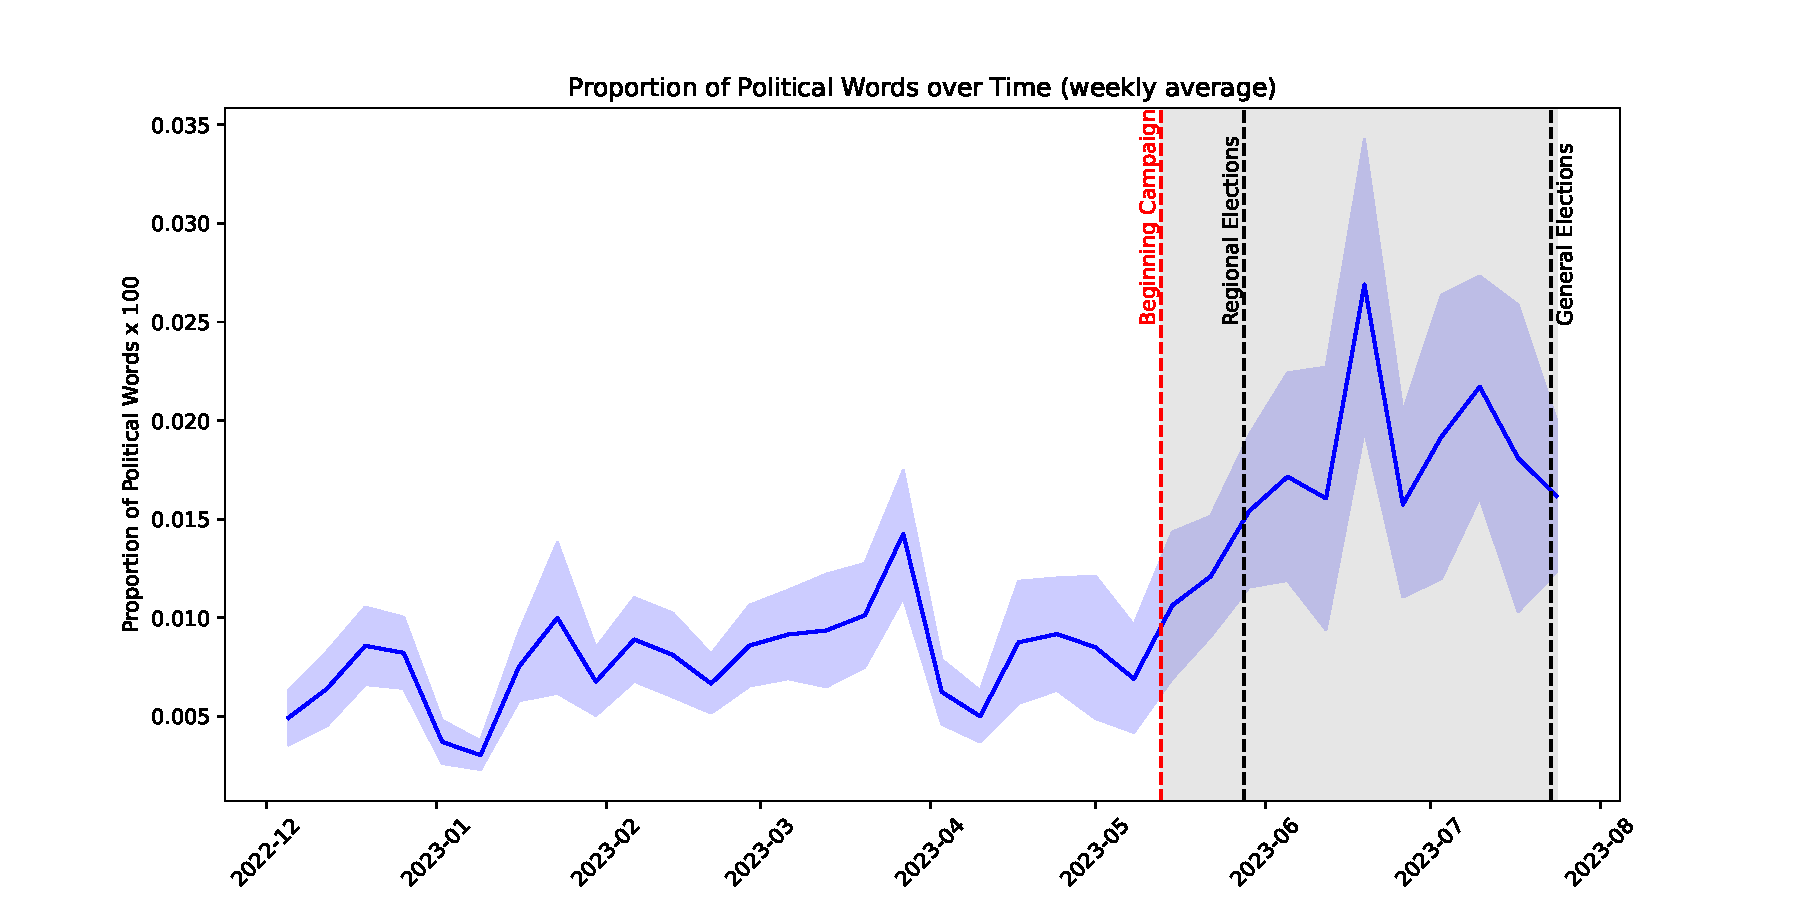
\includegraphics[width=120mm]{figures/political_words2}
		\caption*{\small Notes: Average daily proportion of political terms relative to overall words with shaded standard deviations. Political time is measured by dictionary matches to terms in Table \ref{table:politics}. Vertical, dashed lines indicate the date of the regional and general elections, respectively. The shaded area represents the "campaign" period considered.}
		\label{fig:coverage}
	\end{figure}
	
	
	\subsection{Political Tone}
	
	\label{sec:classification}
	
	Here I describe the methodology used to classify the political tone of the content broadcast. Under market equilibrium, an outlet's slant should match its audience's political leaning. Because the slant classification is unsupervised, I use survey data to evaluate the ideology of each channel's viewers and then use this benchmark to validate the slant classification.
	
	\subsection*{Political Orientation of the Audience}
	
	Figure \ref{fig:opinion} shows the correlation between individuals' preferred political party and their preferred channel for acquiring political information, based on survey data from the Centro de Investigaciones Sociológicas (CIS). Right-wing individuals (PP and VOX) tend to watch Antena 3 more, whereas left-leaning individuals are divided between LaSexta and the public channel TVE. Telecinco appears in the middle, with weak correlations.
	
	
	\begin{figure}[h!]
		\centering
		\caption{Correlation between preferred channel and political party}
		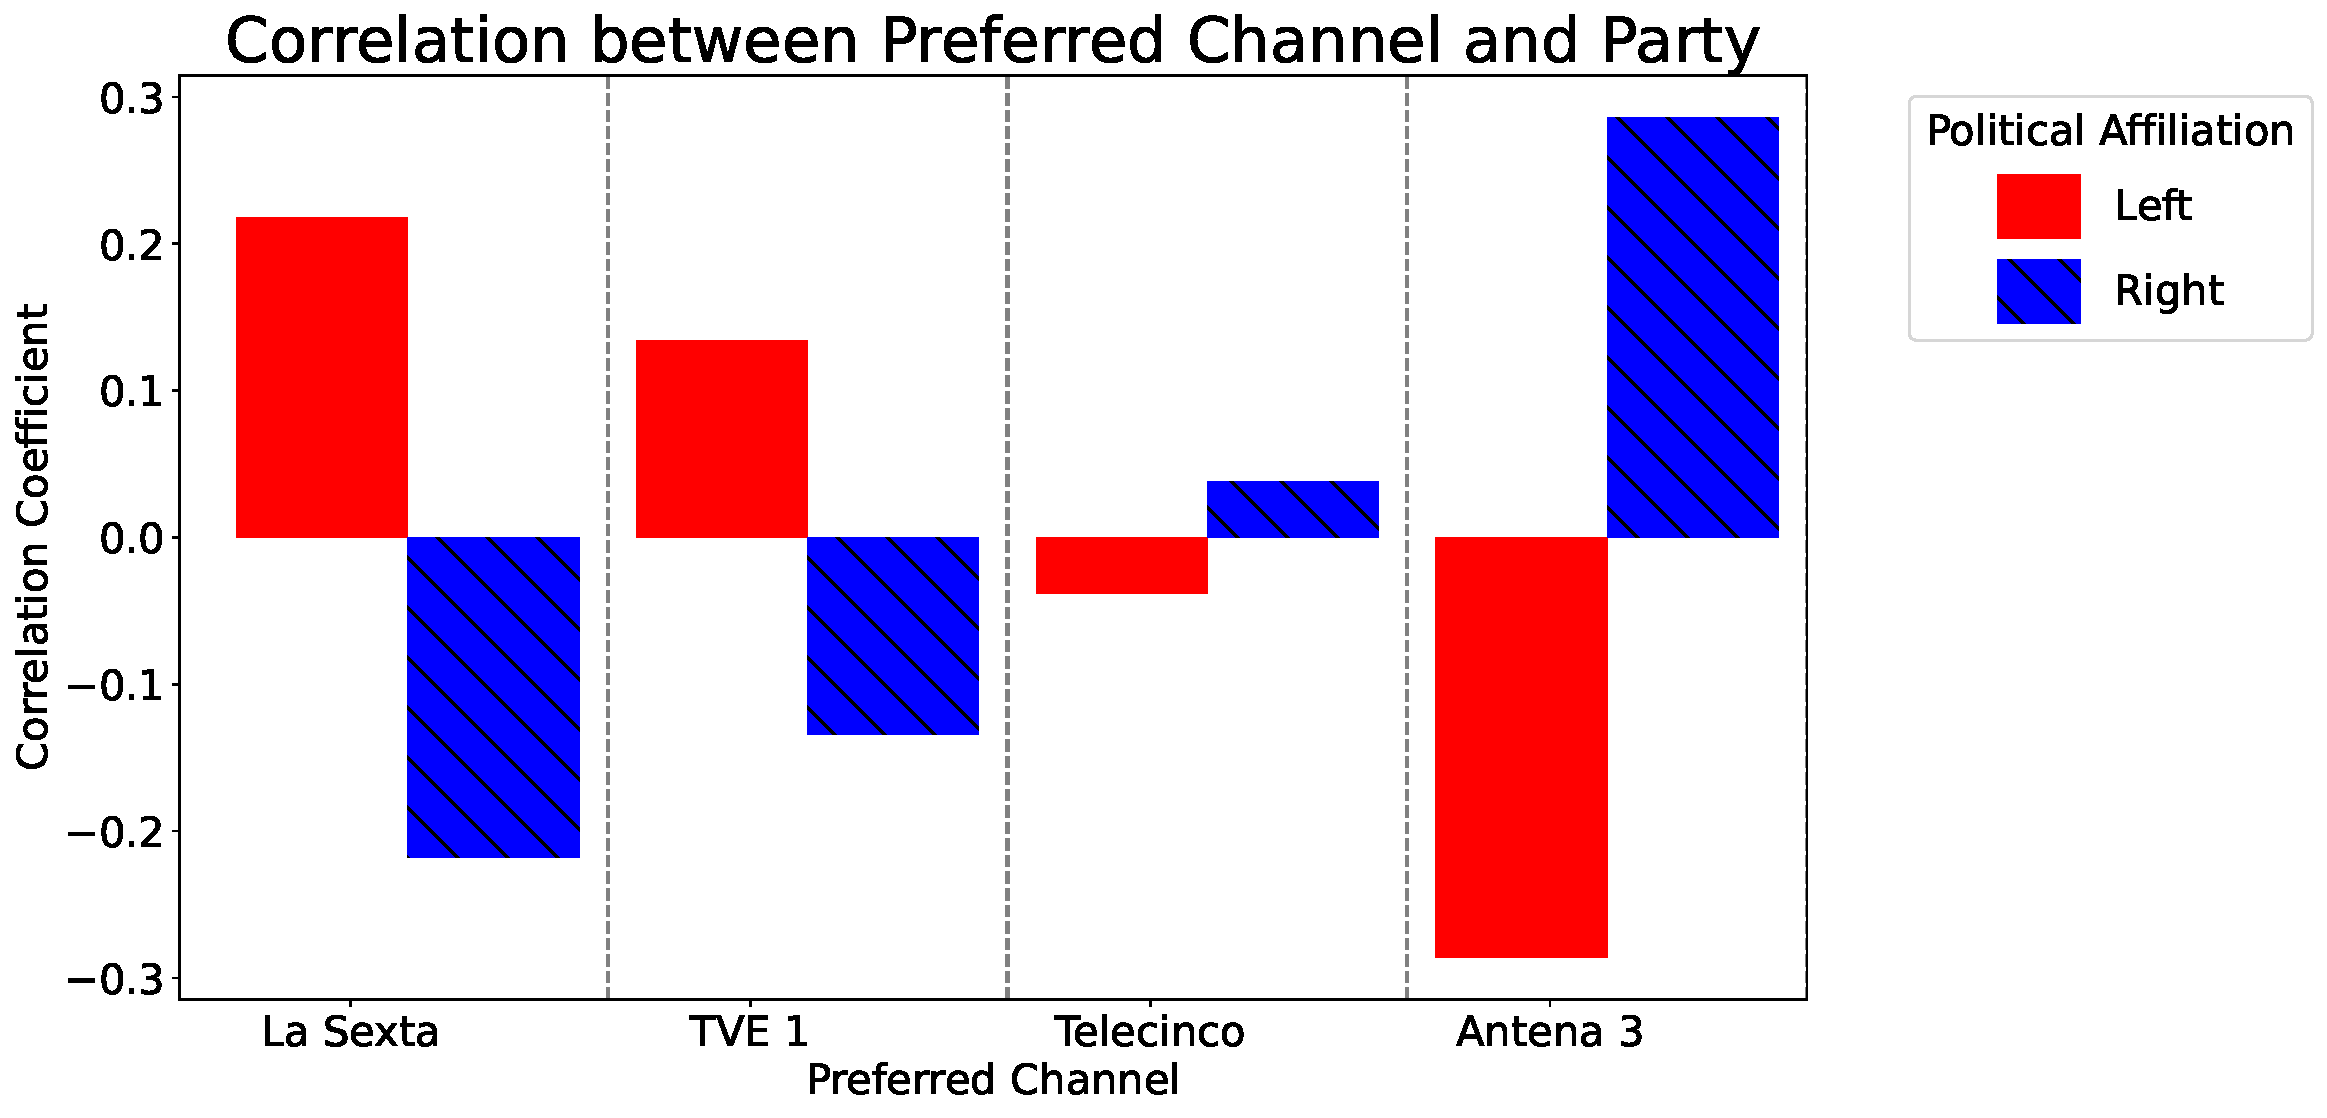
\includegraphics[width=120mm]{figures/corr_party_channel3}
		\caption*{\small Notes:  Bars represent a correlation coefficient between the declared preferred political party (pooling left and right parties) and the most watched channel. The survey ask respondents if they watch TV for political content and what is their preferred channel. Source: Built using data from CIS's Encuesta Pre-electoral 2023 }
		\label{fig:opinion}
	\end{figure}
	Given the well-known issues with survey data for media consumption \citep{prior}, I rely on audience shares together with regional intention-to-vote pools. Figure \ref{fig:density} shows the political density on the left–right spectrum of each channel. The left–right positions of the outlets are consistent with those shown in Figure \ref{fig:opinion}. Given the significant ideological sorting across outlets, I now present the content classification for the outlets’ slant (supply) and compare it with viewer's ideology. 
	
	\subsection{Text Classification}
	
	Text analysis methods, such as party mentions or sentiment analysis, cannot reliably discern named entities. To discern slant in a given story, there must be sufficient context on the theme, political actors involved, irony, etc. The use of LLMs as classifiers has gained popularity in recent years for various contexts, such as the classification of political stances \citep{lemens}, and has even been found to achieve higher precision and accuracy scores for ideological classification compared to human annotators \citep{tornberg2023}. I use ChatGPT-4o, feeding it all of our political stories and asking it to classify the tone associated with each political party. Notably, I distinguish between positive and negative tones toward each party, and I provide a flexible query that allows the classifier to remain neutral if the content is ambiguous. More details about the prompt and classification results can be found in Appendix \ref{sec:chat_gpt}. I describe below how I combine airtime with tone to build content characteristics.
	
	\textbf{Building Content Characteristics}\\
	Each day, channel~$j$ produces a set of stories $S_{jd}$ indexed by~$s$. Empirically, these segments result from BERTopic clustering on the unstructured transcripts, which ensures that the LLM has enough context by feeding it the entire text of a given story. The subset of political stories, $\mathcal{P}_{jd} \subseteq S_{jd}$, is the set of all stories that mention national parties or prominent politicians, identified by keyword matches from Table~\ref{table:politics} in addition to general words related to politics.
	
	Each $s \in \mathcal{P}_{jd}$ is fed into ChatGPT and is assigned a tone $tone(s) \in \{-1,0,1\}$. Stories with a stance (i.e., $tone(s) \in \{-1,1\}$) also receive a party label $p(s) \in \{L,R\}$, whereas neutral stories do not. Notice that the broad classification of what is \textit{political} allows for stories that do not contain any specific mention of Spanish politics to have an associated slant toward some party. Table \ref{tab:international} contains examples of stories that do not match any Spanish political term but still have an associated slant toward a political party. These include favorable economic forecasts from the European Commission, international visits by the Spanish King, or European funds.
	
	A story can be mapped to its duration in minutes, $min(s)$. This is key to accounting for the intensive margin. Combining all these characteristics—i.e., party label, tone, and minutes—I define the shares of positive and negative minutes, as well as the share of airtime devoted to politics, as follows:
	
	


		\begin{equation}\label{eq:controls}
		\begin{aligned}
			x_{jd}^{party+}&= \frac{1}{min_{jd}} \sum_{s \in S_{jd}}\bigg(\mathds{1}\{tone(s)=1\} \times \mathds{1}\{p(s)=party\}\times min(s) \bigg) \quad \forall party \in \{L,R\} \\
			x_{jd}^{party-}&= \frac{1}{min_{jd}} \sum_{s \in S_{jd}}\bigg( \mathds{1}\{tone(s)=-1\} \times \mathds{1}\{p(s)=party\} \times min(s)\bigg) \quad \forall party \in \{L,R\} \\
			x_{jd}^{political}&=\frac{1}{min_{jd}} \sum_{s \in P_{jd}}min(s) 
		\end{aligned}
	\end{equation} 
	
	These variables will constitute the main controls on the empirical application in the next section.  Figure \ref{fig:chat} shows the net average tone relative to total time spent on politics  for each party-outlet. Whilst all channels present a negative net tone on the right, there are still significant differences that allow to map them into a different political spectrum. Both La Sexta and the public channel, TVE, offer more pro-left content. Telecinco appears in the middle but still maintains a pro-left stance and Antena 3 is the only one with a more pro-right balance. 	 
	
	

	
	\begin{figure}[ht!]
		\caption{Average sentiment across channels and parties}
		\centering
		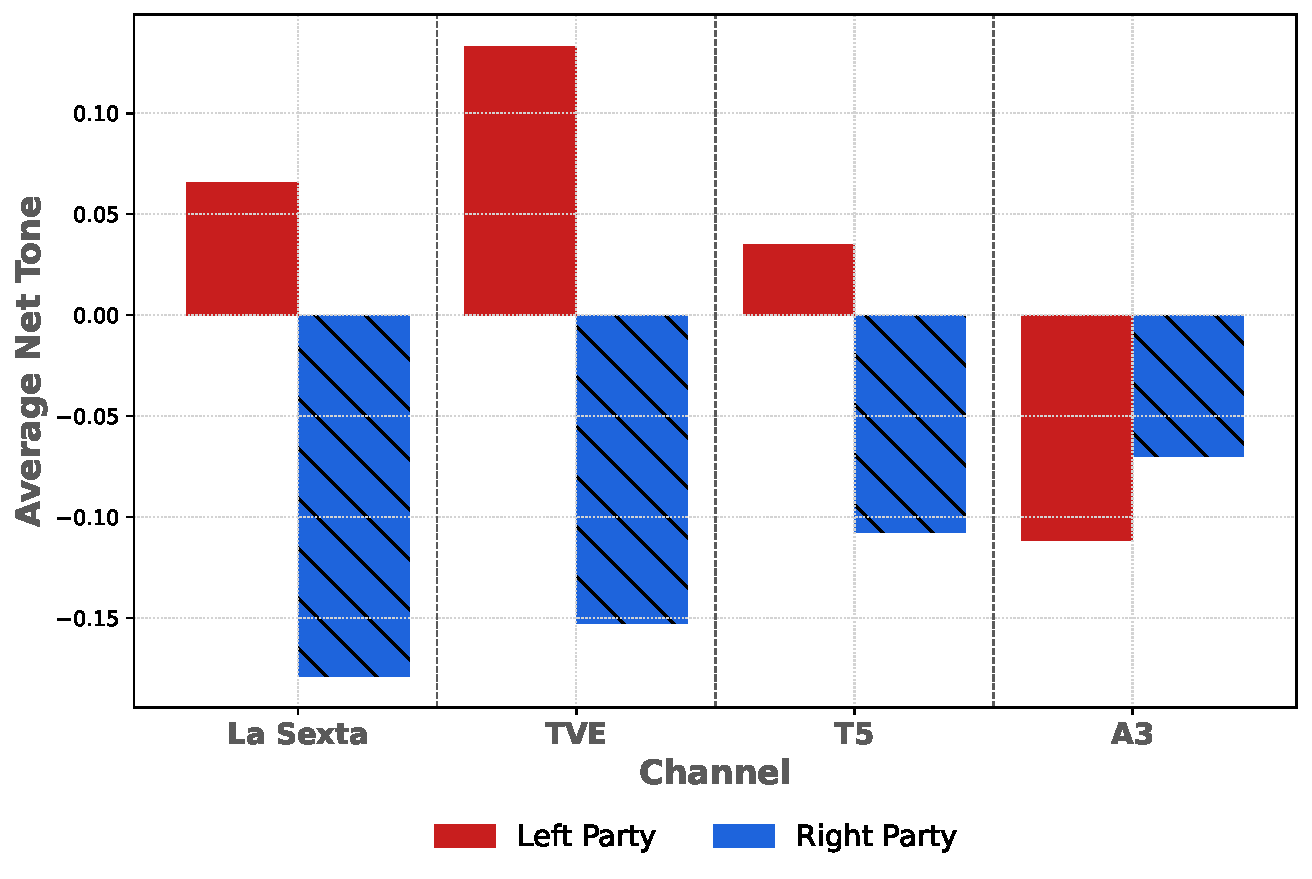
\includegraphics[width=120mm]{figures/chatgpt}
		\caption*{\small Notes: Average tone for each channel-party as classified by Chat GPT 4 from the whole sample period. }
		\label{fig:chat}
	\end{figure}
	
	The results match closely those from declared survey data. 	To simplify the comparison, I assign each channel an ideological score from text as :
	
	\begin{equation}
		\begin{aligned}
			& \frac{\bar{x}_j^{R+}-\bar{x}_j^{R-}-\bar{x}_j^{L+}-\bar{x}_j^{L-}}{\bar{x}_j^{political}}
		\end{aligned}
		\label{eq:position}
	\end{equation} 
	
	
	and, similarly, from the individual survey data, I use the differences in correlation coefficients between right parties. To enable comparisons in positions across scales; I normalize the values of the most to extreme channels to -1 and 1, respectively. 
	
	
	Figure \ref{fig:channel_ideology_lines} panes a) and b)  shows the scores according to viewer's ideology and channels slant; respectively. As expected, the slant offered in the TV news closely matches the viewer's political preferences as one would expect in equilibrium. Below, I show robustness of the text classification and comparison with other methodologies previously used in the literature. 
	
	
		\begin{figure}[ht]
		\centering
		\caption{Normalized Ideology Scores by Channel}
		% Panel (a): ChatGPT-based
		\begin{minipage}[t]{0.48\textwidth}
			\centering
					\textit{(a) Demand: Viewers' ideology}
		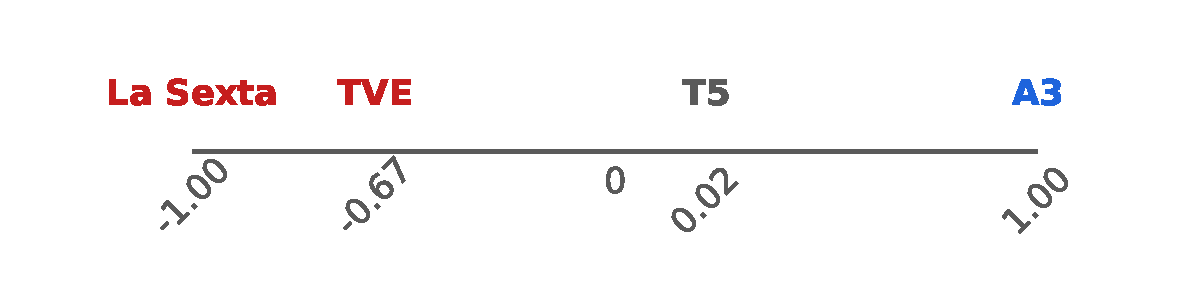
\includegraphics[width=\linewidth]{figures/congress_line_cis}
		\end{minipage}
		\hfill
		% Panel (b): CIS-based
		\begin{minipage}[t]{0.48\textwidth}
			\centering

			
				\textit{(b) Supply: ChatGPT text classification}
			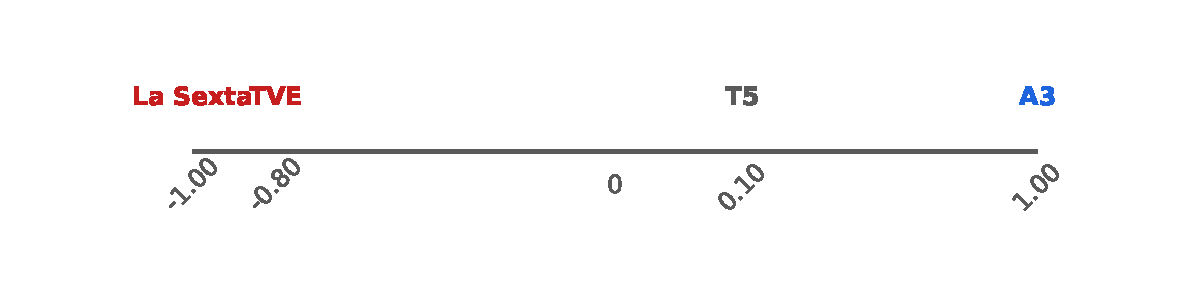
\includegraphics[width=\linewidth]{figures/congress_line_chatgpt}
			
			
		\end{minipage}
		
		
		\caption*{\small \textit{Notes:} The figure compares normalized left–right audience positions for Spanish television channels. Panel (a) uses ChatGPT-based text classification from equation \ref{eq:position}; panel (b) uses viewer ideology data from CIS survey data using the difference in correlation coefficients between right and left. The two most extreme channels are normalized into the -1 and 1 values. }
		\label{fig:channel_ideology_lines}
	\end{figure}
	
	
\textbf{Robustness of the Text Classification}

Two main concerns arise with the use of LLMs as text classifiers. First, LLMs have been shown to suffer from potential stochasticity, making results unstable when using multiple runs of the same prompt. Second, one may question the performance of alternative text classification methods.

Due to their inherent stochasticity, repeated queries using the same prompt may yield different classifications \citep{llmstability2024}. As shown in \citep{llmclassification2024}, this variability can introduce noise in tasks that require high consistency, particularly in content classification. To mitigate this issue, I leverage OpenAI’s “functions” tool, which constrains the classifier’s responses to predefined discrete numerical outputs, reducing potential inconsistencies. Table \ref{tab:table_stability} presents the mean classification scores from 100 iterations of a random sample of political stories, along with the corresponding standard errors. The relatively small standard errors suggest that, despite the model’s stochastic nature, the classification remains stable.

The second concern challenges the validity of LLM reasoning as a tool for political classification. To assess robustness, I compare the LLM’s classifications with those obtained using methods from previous works. I use all Spanish congress speeches during my sample period and exploit party labels to assess similarities with the outlets’ content \citep{gentzkow2010media,laver2003extracting}. Appendix \ref{sec:sent_stability} details the methodology. Importantly, Figure \ref{fig:congress_line} shows the left–right positions derived from this method, which consistently map to the ChatGPT classification in Figure \ref{fig:chat}, confirming the approach’s validity.

\textbf{Political Tone and Electoral Campaign}

The nature of political news during campaigns differs markedly from that off-campaign. Off-campaign stories might cover scandals, international summits, etc., whereas during campaigns politicians specifically aim to gain votes through public speeches. To examine how this affects channels’ slant positions, I decompose the relative tone before and during campaign periods in Figure \ref{fig:tone2}. The left-leaning channel, LaSexta, significantly reinforced its position by increasing its positive tone toward left-wing parties and decreasing it toward right-wing parties. A similar strengthening occurs in the middle channel. Both the public channel and the right-wing outlet significantly moderated their relative slants. Figure \ref{fig:change_line} shows the change in positions relative to off-campaign. Dots mark the normalized –1 to 1 positions from the pre-campaign period, and crosses mark those from the campaign period. The ranking shifts: LaSexta is now the most left-leaning channel, followed by TVE. All but the public channel moderated their tones toward more left-wing–favorable coverage.



\begin{figure}[ht!]
	\centering
	\caption{Change in positions off-campaign to campaign}
	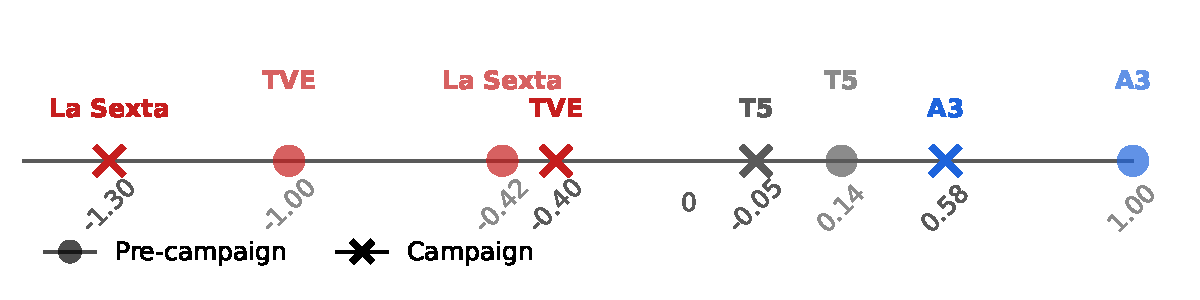
\includegraphics[width=100mm]{figures/congress_line_chatgpt_pre_post}
	
	\caption*{\small \textit{Notes:} The figure shows the relative change in  positions of the slant from off-cmapaign to campaign according to the ChatGPT classification. 			Channels are mapped into the $[-1,1]$ scale using their correlation (tone) and normalizing values into this scale. }
	\label{fig:change_line}
\end{figure}

\textbf{Text vs.\ Image}

Imagery is a key component of TV. Previous work has linked politicians’ appearances on TV to voting outcomes \citep{tv_appeareance}. Below, I compare different metrics of image appearances, politician mentions, and tone.

Due to computational constraints, I cannot perform image detection across my full video sample. Instead, I compare image-based and text-based metrics using a random sample of 67 days. The image-based metric approximates screen time—i.e., the number of seconds a political leader appears visually—and is conceptually similar to the measures constructed in \cite{CageHengelHerveUrvoy2022} and \cite{durante2012partisan}.

Specifically, I train a state-of-the-art face recognition system \citep{face_recognition} using labeled images of the main party leaders: Pedro Sánchez (PSOE), Alberto Núñez Feijóo (PP), Santiago Abascal (VOX), and Yolanda Díaz (UP). I then extract frames from the first 25 minutes of each prime-time news broadcast across major channels, resulting in a sample of 79,788 images. Using the \texttt{face\_recognition} library, I detect and identify faces in each frame. This allows me to construct a frame-level dataset of visual exposure and emotional tone, which I aggregate at the daily level for each channel and party leader.

Figures \ref{fig:image_channel} and \ref{fig:mentions_channel} show the proportions of image appearances and word mentions by channel and political leader. Figure \ref{fig:tone_channel} shows the net tone by political party over the same sample period.

All channels except Telecinco coincide in their ranking of politician visual appearances, with Feijóo first, followed by Sánchez, Díaz, and finally Abascal. Telecinco shows the greatest airtime devoted to Díaz, with her appearing in 3\% of the news. The comparison with the text mentions in Figure \ref{fig:mentions_channel} reveals a different scenario: left-leaning channels mention Díaz relatively more than Sánchez, but this pattern does not hold for the right-leaning channel.

To examine the relationship between tone—based on the LLM classification—and coverage, I regress net tone by political actor on both the proportion of image appearances and word mentions. Tables \ref{tab:feijoo_images} through \ref{tab:diaz_images} report results under different specifications, including date and channel fixed effects.

Column~(4) reports the specification with both channel and date fixed effects, so the coefficients reflect pure within–channel–day fluctuations in coverage. The pattern is heterogeneous across politicians. For Abascal (VOX), a one-standard-deviation increase in word mentions predicts a decrease of $0.28$ standard deviations in tone, whereas the same increase in on-screen images predicts an increase of $0.13$ standard deviations. Sánchez (PSOE) exhibits the reverse pattern: additional text is linked to a $0.11$ standard-deviation softening of tone, while extra images correspond to a $0.13$ increase. Taken together, the results indicate that text-based and image-based measures of salience relate to tone in systematically different ways. This poses concerns regarding the interpretation of previous metrics based on airtime; whereas basic count matches naturally present a noisier predictor of tone, image appearances seem to be consistently associated with a negative, rather than a positive, tone. Further research might explore the integration of imagery and stance.



	
	
	
	\section{Market set up}\label{section:market}
	
In this section I introduce my market set up for demand. Supply will be explicitly modeled in section \ref{sec:supply}. There are no adds during the TV news programs so I abstract from two sided market considerations. Channels differentiate themselves through the way they present the stories of the day. I follow a mixed logit model \citep{berry1994estimating} (BLP) estimation\footnote{The model is estimated under the \textit{pyblp} package \citep{conlon2020best}.}. A key assumption in this type of models is single product choice. TV, however, has strong switching behavior where viewers can explore different alternatives and this cannot be identified from daily, aggregate data. To minimize this concern, I make use of the initial (i.e minute-0) audience of each day. Since 3 out of 4 outlets coincide in their airing times, this makes the single product choice assumption less problematic under the initial audience. 

	An individual $ i $  a region $r$ chooses an outlet $ j \in \mathcal{J}\equiv \{La6,TVE,T5,A3\}$ \footnote{Although both LaSexta and A3 belong to the same media company, AtresMedia; the analysis here is based on short run profit maximization and they are assumed to be different, independent products. } to watch at the beginning of day $d$ based on the following expected utility : 
	
	
	\begin{equation}\label{eq:utility}
		\begin{aligned}
			& U_{ijrd}= \underbrace{\sum_k x_{jd-1}^k\beta^k+w_{rd}   \gamma  +  \xi_{jrd}}_{\delta_{jrd}}  + \underbrace{  \sum_k x_{jd-1}^k \Big( \sigma^k \nu_{ird}^k  + \pi^ky_{irm} \Big)}_{\mu_{ijrd}}+\epsilon_{ijrd} 
		\end{aligned}
	\end{equation} 
	
	where $ x_{jd}^k $ represents the  proportion of time on channel $ j $ and day $ d$ devoted to characteristic $ k \in \{R+,R-,L+,L-,political\}$ as defined in Equation \ref{eq:controls}. $w_{rd}$ measures the precipitation level on a given day-region. Weather conditions alter the value of the outside option and make viewers more prone to engage in indoor activities like TV consumption \citep{wilbur}. In my model, this happens with a common shift in the valuation of the inside options. 
	
	I model the distribution of viewer's content taste parameters using the standard normal random shocks $ \nu_{ird}^k \sim N(0,1)$ with mean shifted by  demographics, $ y_{irm} $, that represent whether individual $i$ is right wing in month $m$ according to survey data.	The parameters $\pi^k$ allow for asymmetric tastes of politics based on ideology. Thus, they capture polarization in news consumption: More right wing individuals might screen out opposed content. 

The unobserved (to the econometrician) product characteristics are decomposed into $\xi_{jrd}= \xi_j + \xi_{dow} + \Delta \xi_{jrd}$, where I include product dummies that account for unobserved quality factors and day of the week dummies to control for  seasonal variation in the value of TV consumption. Unobserved product tastes can take the form of higher valuation of a given type of story that comes from knowledge of it through social media or specific regional taste shocks due to local events. By assumption, both the outlets and the viewers have full information about all the product characteristics. Due to timing differences, this assumption comes in the form of a correct expectation formation for next day unobserved preferences $ \xi_{jrd+1}$ in the moment of setting todays' content $\bm{x_{jd}}$. 
	
	The outside option is modeled in terms of \textit{potential} audience  \citep{berry1994estimating} and its mean utility value is normalized to 0 .
	
	Market shares are just the integral over the individual choice indicators from \ref{eq:utility}:  
	
	
	\begin{equation}\label{eq:shares}
	\begin{aligned}
		& s_{jrd} = \int d_{ijrd}(\bm{\delta_{rd}},\bm{\mu_{ird}})d\bm{\mu}_{ird}d\bm{\epsilon}_{ird}
	\end{aligned} 
\end{equation} 
	
	where $d_{ijrd}$ equals $1$ if $U_{ijrd}>U_{ikrd} \quad \forall j\neq k$ and $0$ otherwise. Survey weights are included in the integration. 

Under the assumption of no individual heterogeneity in preferences  (i.e $\bm{\sigma}=0$) nor in  the distribution of ideology in a given region $y_{ir}= \bar{y_r}$,  equation \ref{eq:utility} is consistent with a plain logit model as:


\begin{equation}\label{eq:logit}
	\begin{aligned}
		& ln \left(\frac{s_{jrd}}{s_{0rd}}\right)= \sum_k x_{jd-1}^k\beta^k+w_{rd}   \gamma  +\sum_k \left(x_{jd-1}^k\times y_r \right) \phi^k +  \xi_{jrd}
	\end{aligned} 
\end{equation} 


I show results under both the BLP and plain logit in  section \ref{section:results}. 
	
	\subsection{Content endogeneity and news shocks} \label{section:endogeneity}
	
	
Previously, demand estimation has often treated content characteristics as exogeneous and use them to instrument for prices. However, my set up precisely shows the adaptation of content to audience preferences: channels tilt the slant of the day and viewers choose their preferred content accordingly. 
	Figure \ref{fig:diagram} depicts the core trade-offs. Viewers form expectations about the utility of each channel based on exogenous variables—weather, individual attributes, and an unobserved (to the econometrician) shock~$\xi$—as well as on yesterday’s content slant~$\bm{x}_{jd}$.  
	Channels, in turn, choose today’s slant while forecasting tomorrow’s utility shock~$\Delta\xi_{j,d+1}$.  
	Hence their optimal content decisions are functions of unobserved taste shocks, implying $\E[\mathbf{x}_{jrd-1}\,\Delta\xi_{jrd}] \neq \mathbf{0}$.
	
	To overcome this problem I instrument, for every endogenous product characteristic~$k$, with exogenous supply shocks.  
	I proxy the daily news landscape with all stories published in Spanish by \emph{Agencia EFE}—around $N\!\approx\!41{,}000$ items over the sample.  
	Television stations rely heavily on third-party wire services for footage, text, and images, a downstream flow documented and exploited in earlier work \citep{milena}.  The fact that all outlets in my sample contract with EFE, mitigates concerns that the agency is systematically biased or poorly informed. 
	
	Mirroring the content covariates in~\eqref{eq:controls}, I classify every EFE story with the same NLP pipeline and construct daily measures of the political mix in the \emph{news landscape}:
	
	\begin{equation}\label{eq:first_stage}
		\begin{aligned}
			z_d^{\,party+} &= \frac{1}{|S_d|}\sum_{s\in S_d}
			\bigl[\mathds{1}\{tone(s)=1\}\,\mathds{1}\{p(s)=\textit{party}\}\bigr]
			&\forall\,\textit{party}\in\{L,R\},\\
			z_d^{\,party-} &= \frac{1}{|S_d|}\sum_{s\in S_d}
			\bigl[\mathds{1}\{tone(s)=-1\}\,\mathds{1}\{p(s)=\textit{party}\}\bigr]
			&\forall\,\textit{party}\in\{L,R\},\\
			z_d^{\,\text{political}} &= \frac{|\mathcal{P}_d|}{|S_d|}.
		\end{aligned}
	\end{equation}
	
	Here $S_d$ denotes the total number of EFE stories on day~$d$, and $\mathcal{P}_d$ the subset classified as political. The \textit{news landscape} is common for all the outlets but will affect them asymmetrically due to their ideal positions. Channels would like to produce at their steady state, average positions (i.e those depicted in \ref{fig:channel_ideology_lines}), but in the short run the available story mix constrains what they can speak about. 
	When the news landscape tilts toward a given party-tone combination, stations are either helped to move closer to—or forced away from—their ideals, depending on how well the available content aligns with those targets. Since days are independent, outlets know they need take profit of a favorable day as newsworthy events might crowd out the news the day after. This setup therefore mirrors the classic BLP strategy of using product-specific cost shifters: the common EFE shock enters each channel’s cost function but, because editorial lines differ, it shifts channels’ content choices differentially within the same day, generating cross-sectional variation that  the  rank condition requires for identification \citep{berry_haile_econometrica}.
	
	
	\begin{comment}
	\begin{figure}[h!]
		\caption{Trade-offs in the model}
		\label{fig:diagram}
		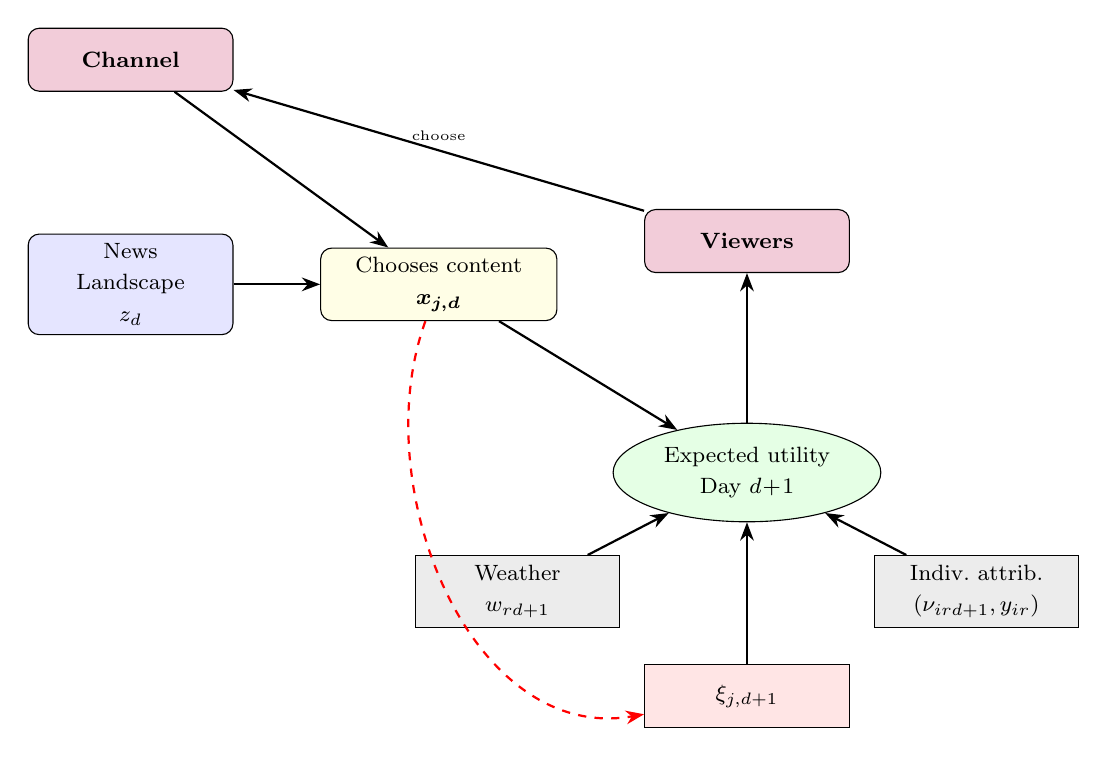
\begin{tikzpicture}[
			inst/.style   ={rectangle, draw, fill=blue!10,  rounded corners, align=center,
				minimum width=2.6cm, minimum height=0.8cm},
			decision/.style={rectangle, draw, fill=yellow!10, rounded corners, align=center,
				minimum width=3.0cm, minimum height=0.9cm},
			util/.style   ={ellipse,   draw, fill=green!10,  align=center,
				minimum width=3.4cm, minimum height=1.0cm},
			shock/.style  ={rectangle, draw, fill=red!10,   align=center,
				minimum width=2.6cm, minimum height=0.8cm},
			exo/.style    ={rectangle, draw, fill=gray!15,  align=center,
				minimum width=2.6cm, minimum height=0.8cm},
			actor/.style  ={rectangle, draw, fill=purple!20, rounded corners, align=center,
				minimum width=2.6cm, minimum height=0.8cm},
			flow/.style   ={-Stealth, thick},
			feed/.style   ={dashed,-Stealth, thick, red},
			node distance = 1.8cm and 1.1cm,
			font=\footnotesize
			]
			% -------- DAY d (supply) ---------
			\node[inst]                    (news)   {News\\Landscape\\$z_{d}$};
			\node[actor, above=of news]    (channel) {\textbf{Channel}};
			
			\node[decision, right=of news] (x)      {Chooses content\\$\bm{x_{j,d}}$};
			
			% -------- DAY d+1 (demand) ------
			\node[actor, right=of x, yshift=0.55cm] (viewer) {\textbf{Viewers}};
			
			\node[util,  below=of viewer, yshift=-0.1cm] (util)
			{Expected utility\\Day $d\!+\!1$};
			\node[shock, below=of util]     (xi)     {$\xi_{j,d+1}$};
			\node[exo,   below left=0.6cm and 0.4cm of util]
			(weather){Weather\\$w_{rd+1}$};
			\node[exo,   below right=0.6cm and 0.4cm of util]
			(prefs)  {Indiv.\ attrib.\\$(\nu_{ird+1},y_{ir})$};
			
			% ---------- flows ---------------
			\draw[flow] (channel) -- (x);
			\draw[flow] (news)    -- (x);
			\draw[flow] (x)       -- (util);
			\draw[flow] (prefs)   -- (util);
			\draw[flow] (weather) -- (util);
			\draw[flow] (xi)      -- (util);
			\draw[flow] (util)    -- (viewer) node[midway,right,font=\tiny]{};
			\draw[flow] (viewer)    -- (channel) node[midway,above,font=\tiny]{choose};
			
			
			% ------ anticipation feedback ---
			\draw[feed] (x) to[out=-110,in=190] node[midway,below,font=\tiny]
			{} (xi);
		\end{tikzpicture}
		\caption*{\small
			Notes: This diagram illustrates the structure of the model. Solid black arrows indicate causal and temporal dependencies among variables. The red dashed arrow emphasizes the simultaneity problem: content decisions $\bm{x}_{j,d}$ are made with knowledge of the future utility shock $\xi_{j,d+1}$.
		}
		
	\end{figure}
	
	
	\end{comment}



Outlets' coverage of scandals or economic  have been extensively documented for the U.S. press  (see e.g. \cite{puglisi2011newspapers, Larcinese2007NBERWP}). Tables \ref{tab:neg_left_channels} and \ref{tab:neg_right_channels} illustrate this mechanism linking the news landscape to outlet's reporting. 
The most unfavourable day for left-wing parties in my sample is 27 February 2023.  
On that date a technical flaw a law sponsored by the left party Podemos; motions and corruption scandals towards the Socialist party hurt the coalition government. 

Airtime devoted to negative left-wing stories therefore spiked: Antena~3 (right) devoted almost 19 \%, while TVE (left) and Telecinco each gave roughly 4 \%, and La Sexta (left) only 2 \%.

The mirror image occurred on 17 May 2023, the day with the most negative coverage of right-wing parties.  
Stories included a payments scandal involving the People's Party, the defeat of a conservative motion in the Senate, and police abuse allegations during an anti-VOX march.  

This time the left wing outlets lead the production of negative right-wing content with 15 \% of the time, whereas Antena 3 devoted barely 4 \%. 


\medskip

In order to show formal evidence of the previous mechanism,  I estimate, for each $(party,tone)$ pair, separate regressions of the form:
\begin{equation}\label{eq:pred_pos}
	\begin{aligned}
		 x^{party, tone}_{jd} =	\sum_{k} 
		\left(\bm d_j \times z^{k}_d\right)\,\alpha_{j}^{k}
		+
		\left(\bm d_j \times z^{political}_d\right)\,\alpha_j^{political}
		+ \epsilon_{jd},
	\end{aligned}
\end{equation}

where $tone,k \in\{L+,R+,L-,R-\}$. As was described before,  $x^{party, tone}_{jd}$ is outlet $j$’s share of airtime with positive or negative tone about \emph{party}, $z^{party,k}_d$ is the corresponding share among all EFE stories, and $\bm d_j$ is a vector of outlet dummies.  Controlling for the whole news landscape, I estimate how outlets increase the production of content of each type. 
A positive coefficient $\alpha_{j}^{R,+}$ means that, ceteris paribus, one additional positive right-wing story in the wire increases outlet $j$’s own positive coverage of the right by $\alpha_{j}^{R,+}$.

Results of the estimation are shown in table \ref{tab:first_stage}. Figure \ref{fig:fwl} presents added-variable plots for regression equation  \eqref{eq:pred_pos} (a LOWESS version appears in Appendix Figure \ref{fig:fwl_lowess}).  

 When the share of  positive-right stories rises by one standard deviation, the right-leaning Antena 3 lifts its own positive-right airtime by about 0.30 stdev., whereas the left-leaning outlets TVE and La Sexta react hardly at all.  Symmetrically, a one-stdev. increase in positive-left stories leads TVE to expand favourable coverage of the left by roughly 0.38 stdev, while Antena 3’s response is indistinguishable from zero.  By contrast, none of the channels shows more than a “small’’ (\(<0.15\) stdev) adjustment to extra negative-right news, consistent with the idea that hostile coverage of the right is already close to saturation (eg. see figure \ref{fig:chat}).


	
	
		\begin{figure}[h!]
		\centering
\caption{Added variable plots for production of political content}
		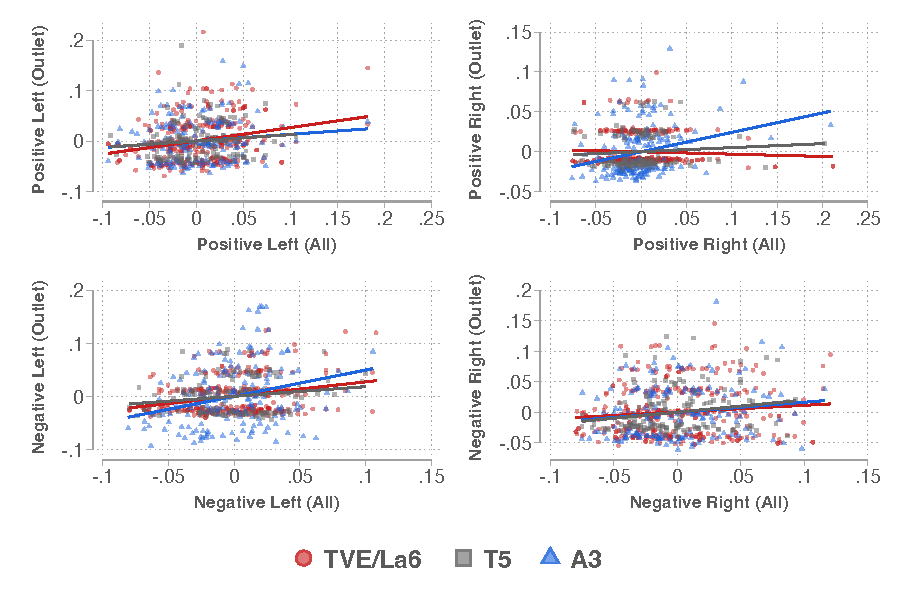
\includegraphics[width=160mm]{figures/fwl_plots}
		\caption*{\small Notes: The figure shows the added variable plots from the estimation of equation \ref{eq:first_stage}. The x axis represents $\left(z_d^{party,+},z_d^{party,-}\right) $ and the y axis the corresponding  $\left(x_{jd}^{party,+},x_{jd}^{party,-}\right) $   . Channels are pooled into left (TVE and La6), middle (T5) and right (A3) for visualization purposes.  }
		\label{fig:fwl}
	\end{figure}
	
	
	
	
	\begin{table}[h!]
		\centering
	
		\label{tab:tests}
		\caption{F and t-tests for Regression Coefficients}
		\begin{tabular}{lcccc}
			\hline
			Characteristic & F-test  & F-test p-value & T-test  & T-test p-value \\
			\hline
			$ {L-}$& 2.69 & 0.0686 & 3.51  & 0.0613 \\
			$ {L+}$ & 1.31 & 0.2711 & 1.87  & 0.1715 \\
			$ {R-}$ & 0.42 & 0.6594 & 0.34 & 0.5592 \\
$ {R+}$ & 8.78 & 0.0002 & 17.55  & 0.0000 \\
			\hline
		\end{tabular}
			\caption*{\small Notes: Summary of F- and T-test results for equality of news variable coefficients across channels. The F-test evaluates overall equality across channels, while the T-test compares the coefficient of the main independent variable between A3 and TVE/La6.}
	\end{table}
	
	
	
	
	Accordingly, I use
	$\bigl(z_d^{party+},z_d^{party-},z_d^{political}\bigr)_{party\in\{L,R\}}$
	as instruments for the linear content characteristics.  The goal is not to proxy the outlet-specific news landscape perfectly, but to exploit exogenous variation in story supply that shifts slant decisions.  
	The short sample window limits any strategic adaptation of EFE’s editorial line to individual channels.
	
	For the $K$ non-linear parameters governing preference heterogeneity I follow \citet{gandhi2019measuring}.  
	Instruments take the form
	$\bigl(\hat{x}_{jd}^k-\sum_{l\neq j}\hat{x}_{ld}^k\bigr)^2$,
	where $\hat{x}_{jd}^k$ is the first-stage prediction from~\eqref{eq:pred_pos}.
	To identify demographic interactions, I multiply these instruments by the local share of right-wing votes, $\bar y_r\,\hat{x}_{jd}^k$.







	\section{Results}
	
	\label{section:results}
	
	I present the results of the BLP estimation for the pre-campaign and campaign periods in Table \ref{tab:results_blp}. I show the preferred specification with outlet and day-of-week fixed effects and standard errors clustered at the regional level.
	
	The pre-campaign estimates reveal four main facts. First, there is a strong, statistically precise mean taste for stories about national politics, indicating that political coverage per se draws audience attention before the campaign begins. Second, conditional on this baseline, viewers demand a negative tone toward both parties, but the pull is considerably stronger when the right-wing bloc is the target, whereas positive-toned stories are, on average, unattractive. Third, there is no sizable dispersion in the taste parameters captured by the estimated $\sigma$. This is expected, as identification of these parameters requires exogenous changes in the choice sets \citep{berry_haile}, which do not apply in my market setup. Fourth, the ideology–content interaction terms are small and imprecise, so the heterogeneity cannot be explained by viewers’ ideology.
	
	During the campaign window, the same specification paints a markedly different picture. The average taste for political coverage becomes negative, suggesting that audiences experience political saturation once the race officially begins. Conditional on this baseline, valence preferences reverse and intensify: viewers now reward positive stories about the left and negative stories about the right while penalising the opposite frames, producing an aggregate tilt toward left-leaning parties. Ideology–content interactions, however, reveal stark polarisation. Right-wing audiences actively seek favourable coverage of their own side and avoid negative stories about it, yet the dominant force is out-group animosity: they exhibit a particularly strong demand for negative coverage of the opposition. This pattern is consistent with \emph{affective polarisation} and echoes evidence from the United States showing that exposure to presidential campaigns makes partisans increasingly hostile toward their opponents \citep{Peterson2017Echo}.
	
	
	
	
	

	\begin{table}[p]
					\caption{BLP Estimation Results with Standard Errors}
					\label{tab:results_blp}
		\centering
		\begin{threeparttable}
			\begin{tabular}{lccc}
				\hline
				\textbf{Coefficient} & \textbf{Parameter} & \textbf{Estimate} & \textbf{Std. Error} \\
				\hline
				\multicolumn{4}{c}{Pre-campaign} \\
				\hline
				\hline
				Positive Left & $\beta^{L+}$ & -16.90 & (11.73) \\
				Positive Right & $\beta^{R+}$ & -25.53 & (31.03) \\
				Negative Left & $\beta^{L-}$ & 28.29 & (25.89) \\
				Negative Right & $\beta^{R-}$ & 56.44** & (28.45) \\
				Political & $\beta^{political}$ & 11.49*** & (4.28) \\
				Weather & $\gamma$ & 0.00 & (0.03) \\
				\hline
				Positive Left & $\sigma^{L+}$ & 0.44 & (296.90) \\
				Positive Right & $\sigma^{R+}$ & 0.68 & (715.26) \\
				Negative Left & $\sigma^{L-}$ & 12.64 & (8.68) \\
				Negative Right & $\sigma^{R-}$ & 21.99 & (13.83) \\
				Political & $\sigma^{political}$ & 0.00 & (46.79) \\
				\hline
				Right-Wing $\times$  Positive Left & $\pi^{L+}$ & 46.26 & (48.70) \\
				Right-Wing $\times$  Positive Right & $\pi^{R+}$ & 77.81 & (95.92) \\
				Right-Wing $\times$  Negative Left & $\pi^{L-}$ & -70.09 & (57.97) \\
				Right-Wing $\times$  Negative Right & $\pi^{R-}$ & -103.71 & (97.76) \\
				Right-Wing $\times$  Political & $\pi^{political}$ & -25.17** & (12.59) \\
				\hline
				\hline
				\multicolumn{4}{c}{Campaign} \\
				\hline
				\hline
				Positive Left & $\beta^{L+}$ & 134.16** & (65.57) \\
				Positive Right & $\beta^{R+}$ & -129.79*** & (48.43) \\
				Negative Left & $\beta^{L-}$ & -104.84** & (41.32) \\
				Negative Right & $\beta^{R-}$ & 92.62** & (41.63) \\
				Political & $\beta^{political}$ & -6.43** & (3.26) \\
				Weather & $\gamma$ & 0.00 & (0.01) \\
				\hline
				Positive Left & $\sigma^{L+}$ & 0.00 & (320.36) \\
				Positive Right & $\sigma^{R+}$ & 19.25* & (10.89) \\
				Negative Left & $\sigma^{L-}$ & 0.00 & (134.33) \\
				Negative Right & $\sigma^{R-}$ & 0.02 & (73.18) \\
				Political & $\sigma^{political}$ & 0.00 & (19.55) \\
				\hline
				Right-Wing $\times$  Positive Left & $\pi^{L+}$ & -421.99** & (176.15) \\
				Right-Wing $\times$  Positive Right & $\pi^{R+}$ & 334.94*** & (127.41) \\
				Right-Wing $\times$  Negative Left & $\pi^{L-}$ & 288.65** & (116.22) \\
				Right-Wing $\times$  Negative Right & $\pi^{R-}$ & -280.33*** & (104.44) \\
				Right-Wing $\times$  Political & $\pi^{political}$ & 19.34** & (8.93) \\
				\hline
				\hline
			\end{tabular}

			\begin{tablenotes}
				\small
				\item \footnotesize{The table shows the results of the BLP estimation of model \ref{eq:utility}. The estimations are divided into the pre-campaign and campaign period. Both day-of-the-week and outlet fixed effects are included. Standard errors are clustered at the region level. The total number of observations are $N_{campaign}=2307$ and  $N_{pre\_campaign}=6604$.}
			\end{tablenotes}
		\end{threeparttable}
	\end{table}
	
	
	
	
	
	
	
	\begin{comment}
	
	\begin{table}[ht]
		\centering
		\begin{threeparttable}
			\begin{tabular}{lccc}
				\hline
				\textbf{Coefficient} & \textbf{Parameter} & \textbf{Estimate} & \textbf{Std. Error} \\
				\hline
				\hline
				\multicolumn{4}{c}{{Pre-campaign}} \\
				\hline
				\hline
				Positive Left & $\sigma^{L+}$ & 7.04 & (21.28) \\
				Positive Right & $\sigma^{R+}$ & 23.82 & (20.06) \\
				Negative Left & $\sigma^{L-}$ & 3.85 & (11.56) \\
				Negative Right & $\sigma^{R-}$ & 25.42*** & (5.01) \\
				Political & $\sigma^{\text{political}}$ & 3.47 & (7.58) \\
				\hline
				Right-Wing $\times$ Positive Left & $\pi^{L+}$ & 21.75 & (16.78) \\
				Right-Wing $\times$ Positive Right & $\pi^{R+}$ & 35.74 & (43.73) \\
				Right-Wing $\times$ Negative Left & $\pi^{L-}$ & -48.27 & (33.58) \\
				Right-Wing $\times$ Negative Right & $\pi^{R-}$ & -63.86 & (48.13) \\
				Right-Wing $\times$ Political & $\pi^{\text{political}}$ & -13.89 & (12.77) \\
				\hline
				Positive Left & $\beta^{L+}$ & -10.88 & (7.41) \\
				Positive Right & $\beta^{R+}$ & -18.19 & (23.08) \\
				Negative Left & $\beta^{L-}$ & 14.41 & (12.51) \\
				Negative Right & $\beta^{R-}$ & 43.11*** & (16.62) \\
				Political & $\beta^{\text{political}}$ & 4.73 & (5.41) \\
				Weather & $\gamma$ & 0.01 & (0.01) \\
				\hline
				\hline
				\multicolumn{4}{c}{{Campaign}} \\
				\hline
				\hline
				Positive Left & $\sigma^{L+}$ & 1.26 & (145.13) \\
				Positive Right & $\sigma^{R+}$ & 33.40 & (42.70) \\
				Negative Left & $\sigma^{L-}$ & 0.38 & (218.79) \\
				Negative Right & $\sigma^{R-}$ & 0.54 & (226.19) \\
				Political & $\sigma^{\text{political}}$ & 2.92*** & (0.90) \\
				\hline
				Right-Wing $\times$ Positive Left & $\pi^{L+}$ & -708.11** & (299.27) \\
				Right-Wing $\times$ Positive Right & $\pi^{R+}$ & 508.87*** & (172.30) \\
				Right-Wing $\times$ Negative Left & $\pi^{L-}$ & 413.36*** & (147.90) \\
				Right-Wing $\times$ Negative Right & $\pi^{R-}$ & -455.86** & (178.69) \\
				Right-Wing $\times$ Political & $\pi^{\text{political}}$ & 27.60** & (12.62) \\
				\hline
				Positive Left & $\beta^{L+}$ & 217.09*** & (76.90) \\
				Positive Right & $\beta^{R+}$ & -190.52** & (89.31) \\
				Negative Left & $\beta^{L-}$ & -145.58*** & (48.63) \\
				Negative Right & $\beta^{R-}$ & 147.49*** & (52.60) \\
				Political & $\beta^{\text{political}}$ & -10.80** & (4.89) \\
				Weather & $\gamma$ & 0.04 & (0.03) \\
				\hline
				\hline
			\end{tabular}
			\caption{BLP Estimation Results with Standard Errors}
							\label{tab:results_blp_updated}
			\begin{tablenotes}
				\small
				\item \footnotesize{The table shows the results of the BLP estimation of model \ref{eq:utility}. The estimations are divided in the pre-campaign and campaign period. Both day of the week and outlet fixed effects are included. Standard errors are clustered at the region level. The total number of observations is $N_{campaign}=2307$ and $N_{pre\_campaign}=6604$.}
			\end{tablenotes}
		\end{threeparttable}

	\end{table}
	
	\end{comment}
	
	
	\textbf{Elasticities}
	
	I present the mean own elasticities across right and left markets for both the off campaign and campaign periods.  Given that increasing the positive relative minutes to a party also implies increasing the overall total minutes on politics, I compute the elasticity for the $k$th characteristic as: 
	
	\begin{equation}\label{eq:elasticities}
		\begin{aligned}
			& \bar{\epsilon}^k= \frac{1}{J\times R \times D}\sum_{j}\sum_{r} \sum_{d} \left(\frac{\partial s_{jrd}}{\partial x_{jt}^k} +  \frac{\partial s_{jrd}}{\partial x_{jt}^{political}} \right) \frac{x_{jd}^k}{s_{jrd}}    \quad \forall k \in \{R+,R-,L+,L-\}
		\end{aligned}
	\end{equation}             
	
	
The estimated elasticities for right and left-markets \footnote{Where a region is define as right if the proportion of right-wing voters is above the median. } across tones are shown in figure \ref{fig:2figsA} for the pre-campaign and campaign periods; respectively. Estimate results are also shown in Table \ref{tab:elasticities} on the Appendix. 

The polarization in preferences clearly emerges in the right pane (b), where it is shown how the right and left markets present opposed elasticities for the tones that opposed their ideological views. 

To give a size effect of this change; an increase of 1 per cent on net tone towards a party (i.e $ \bar{\epsilon}^{party+}- \bar{\epsilon}^{party-}$) is associated with a 0.31 per cent increase in audience share during campaign periods vs a 0.31 per cent decline in pre-campaign.

This means that an in crease of 1 per cent of negative right tone during the campaign is associated with a loss of 8015 total viewers in right markets with respect to the pre-campaign period. 


\begin{figure}[ht]
	\centering
	\caption{Estimated Elasticities for Right and Left markets, Pre-campaign and Campaign}
	
	\vspace{0.5em} % space between caption and figures
	
	\begin{minipage}{0.45\textwidth}
		\centering
		\textbf{(a)} Pre-campaign\\
		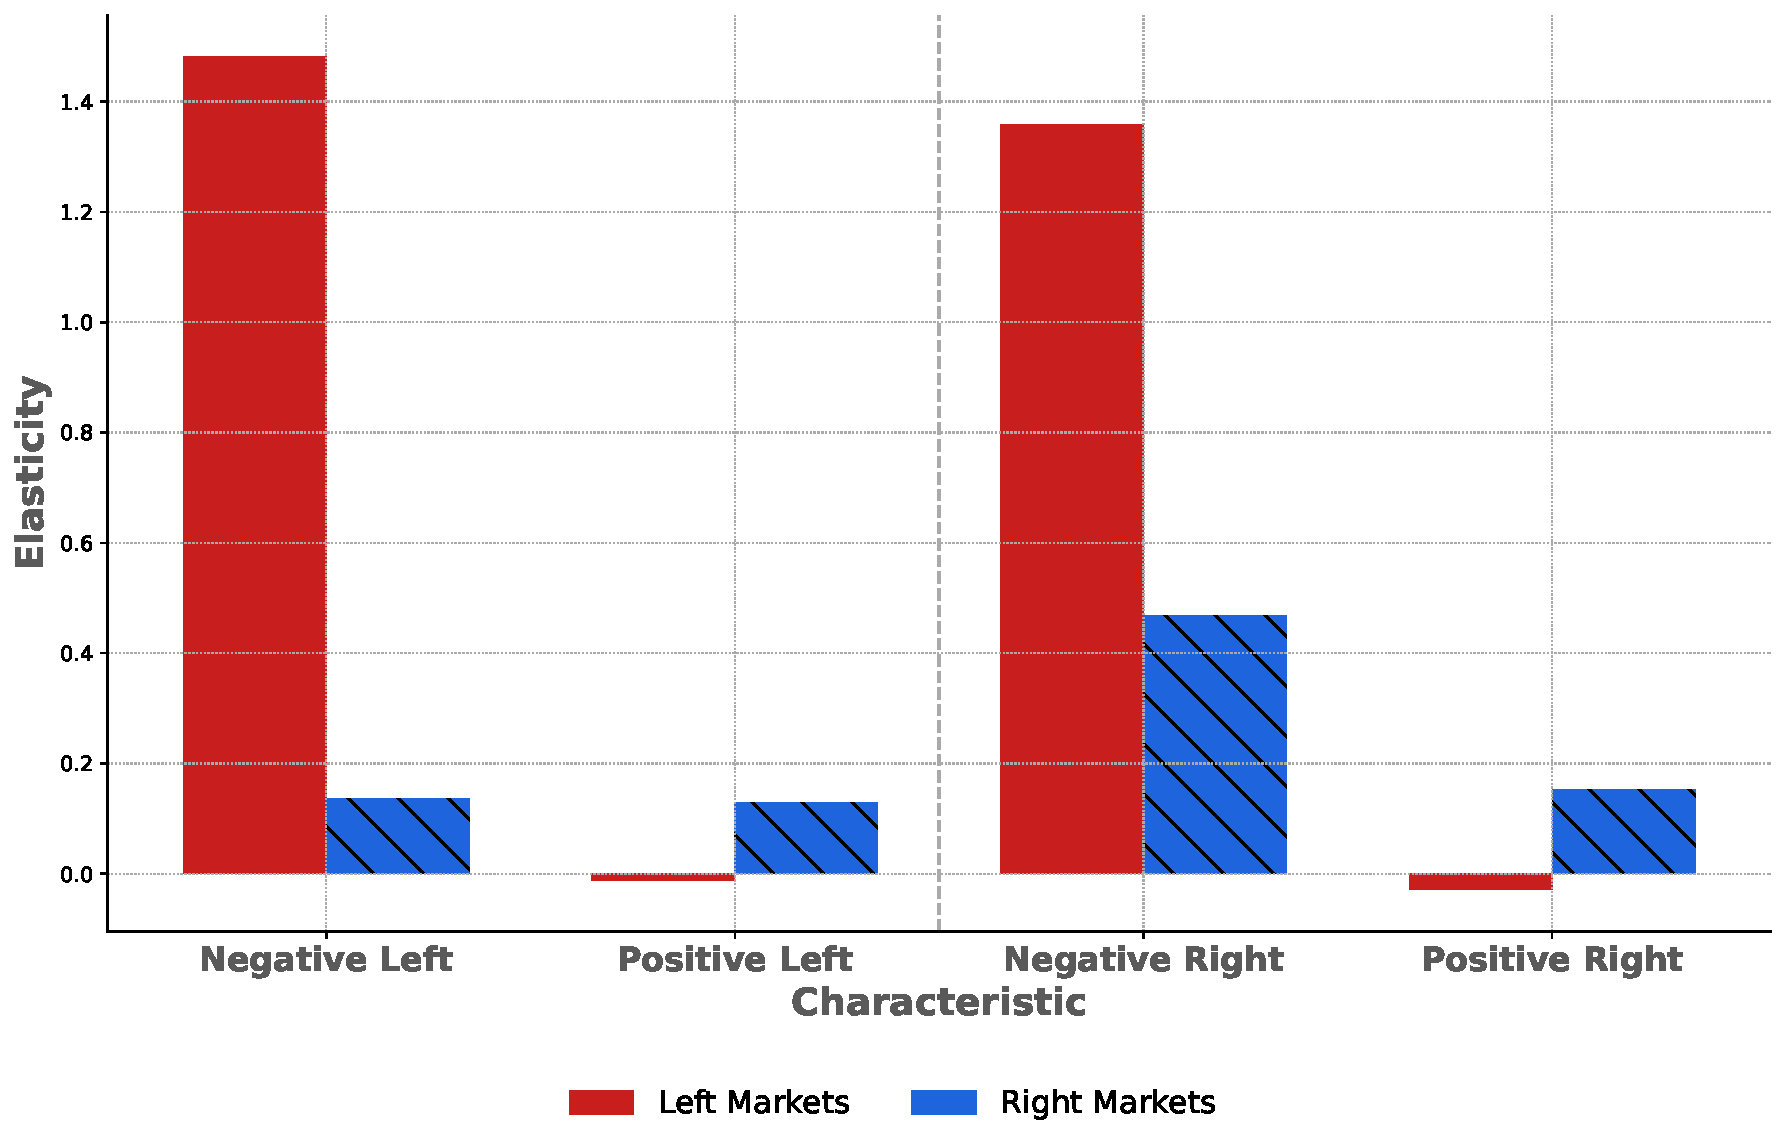
\includegraphics[width=\linewidth]{figures/elasticities_pre_campaign}
%		\label{fig:2figsA}
	\end{minipage}
	\hfill
	\begin{minipage}{0.45\textwidth}
		\centering
				\vspace{1.5em}
		\textbf{(b)} Campaign\\

		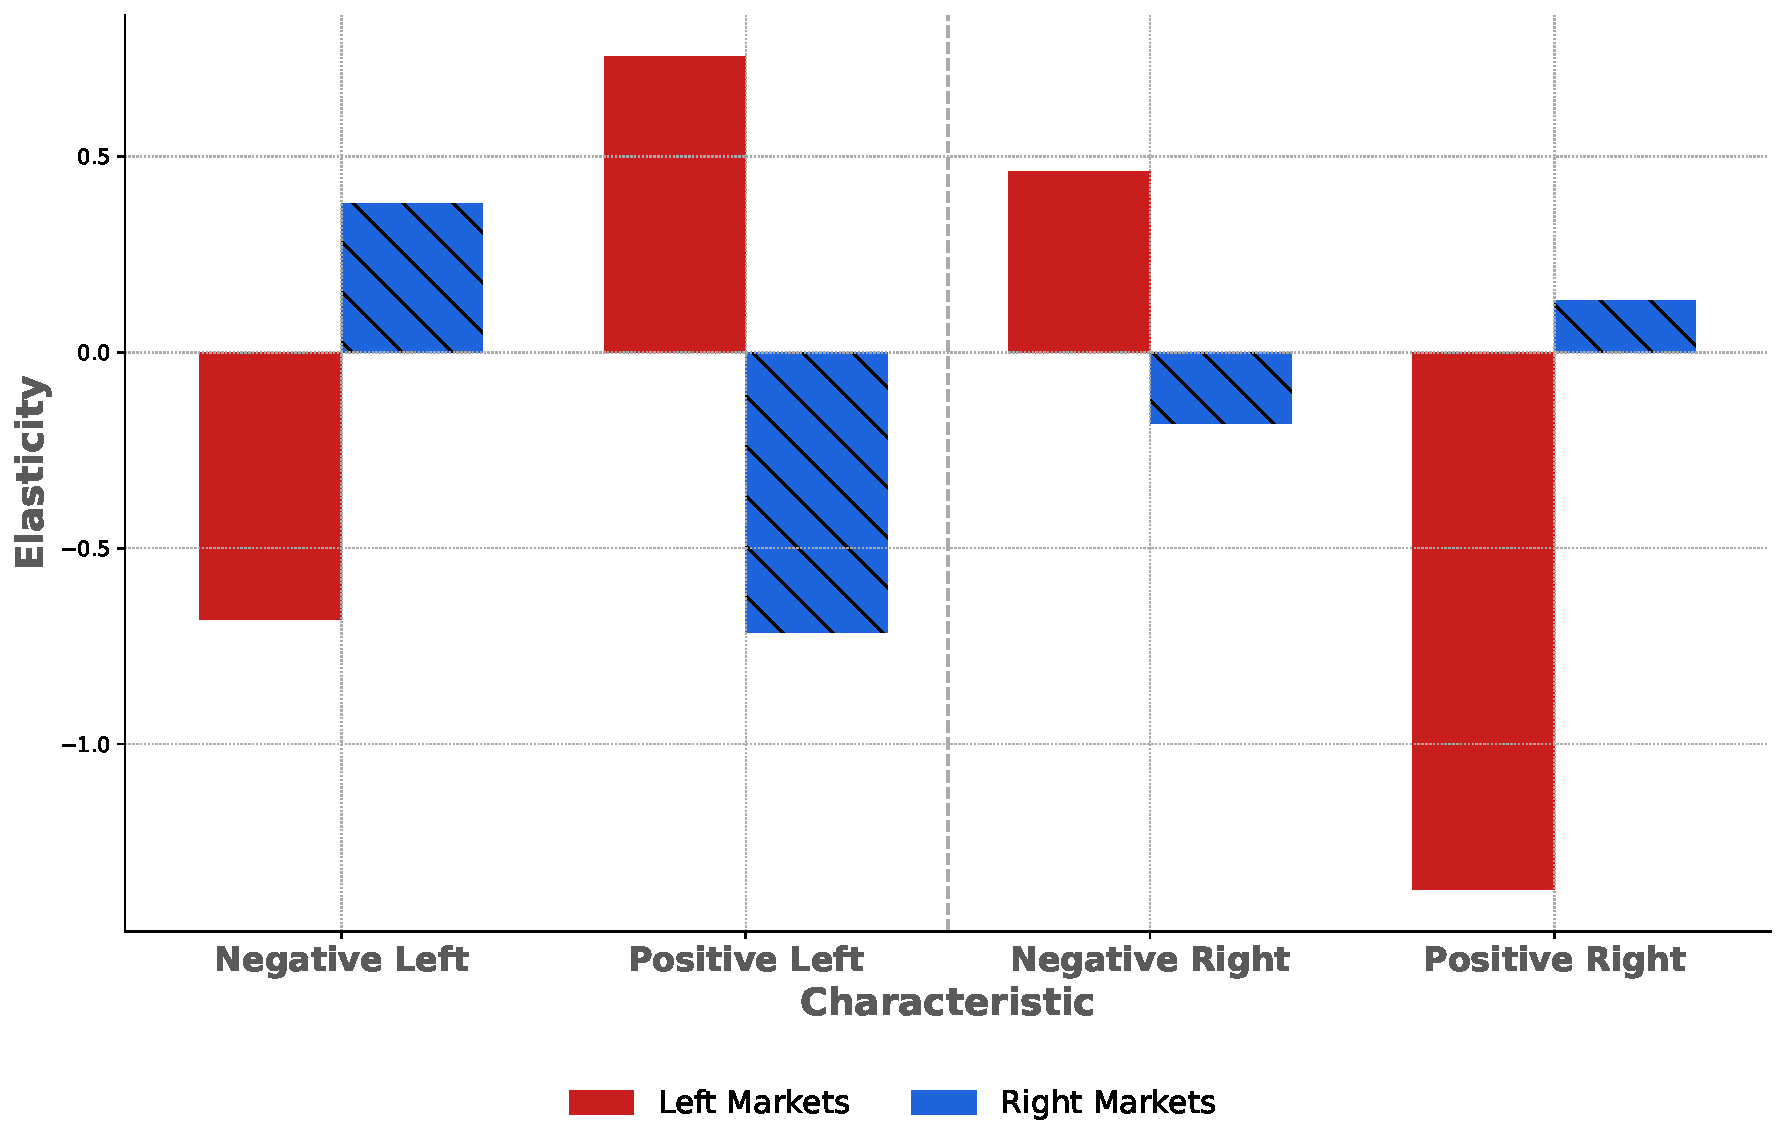
\includegraphics[width=\linewidth]{figures/elasticities_campaign}
		\label{fig:2figsA}
	\end{minipage}
	
	\vspace{0.5em} % space between figures and note
	
	\captionsetup{justification=justified}
	\caption*{\textit{Note:} \small Each panel shows estimated mean own elasticities for consumer responses in right- and left-leaning markets as described in equation \ref{eq:elasticities}. Panel (a) reports results for the pre-campaign period, while Panel (b) covers the campaign period.}
\end{figure}



In order to replicate the outlets' positions shown in figure \ref{fig:channel_ideology_lines}; I do the analogous comparison ranking them according to their estimated demand elasticities. Figure \ref{fig:channel_ideology_lines2} on the appendix shows the comparison. Panel a) ranks channels in the -1,1 segment according to the campaign elasticities. Panel (b) shows their positions for the same period according to their slant. Both rankings agree and the relative scores of the middle channels are similar indicating the consistent equilibrium between supply and demand. 





	\textbf{Political Polarization}
	
	
	

Does the polarization in media consumption link to electoral attitudes?  In this section I show correlational evidence between political and media polarization from my demand estimates. As in \cite{martin2017}, I compute  the Esteban-Ray (ER) polarization index \citep{esteban} using the intention to vote by region as:

\begin{equation}
	ER_{rm}  =	 \sum_{p}   \sum_{q}
	s_{prm}^{\,1+\alpha}\,s_{qrm} \times 1,\qquad \alpha = 1.5,
		\label{eq:er}
\end{equation}

where $s_{pm}$ is the share of intention to vote for party $p\in \{L,R\}$  on month $m$ and I set $\alpha=1.5$. Since there are only two blocks, the distance between political parties is normalized to one. 


Media polarization is captured by the \emph{elasticity gap} between reactions to congenial and uncongenial coverage during the campaign. For right wing regions, $p(r)=R$, media polarization refers to the difference in taste for negative content on the left versus positive and viceversa: 


\begin{equation}
	MediaPol_r  =	\begin{cases}
		\bar{\epsilon}_r^{(L-)}- \bar{\epsilon}_r^{(L+)} \quad if \quad p(r)=R\\
		\bar{\epsilon}_r^{(R-)}- \bar{\epsilon}_r^{(R+)} \quad if \quad p(r)=L
	\end{cases}
		\label{eq:mediapol}
\end{equation}


I divide regions in \textit{high} and \textit{low} groups according to their media polarization index relative to the median. Figure~\ref{fig:er1} plots the smoothed  \(ER_{rm}\)
for both groups over the year before and after the 2023 general election \footnote{Raw time series are shown in appendix figure \ref{fig:er}.}. Places that present higher polarized media consumption coincide with a highly divided electorate. Moreover, consistent with the results in the demand estimation, polarization intensifies close to the moment where the campaign begins. The gap between both high and low regions also widens after the trend break. This feedback reinforces the link between media consumption and voting outcomes. 



\begin{figure}[ht!]

	\centering
		\caption{Political and Media Polarization}
	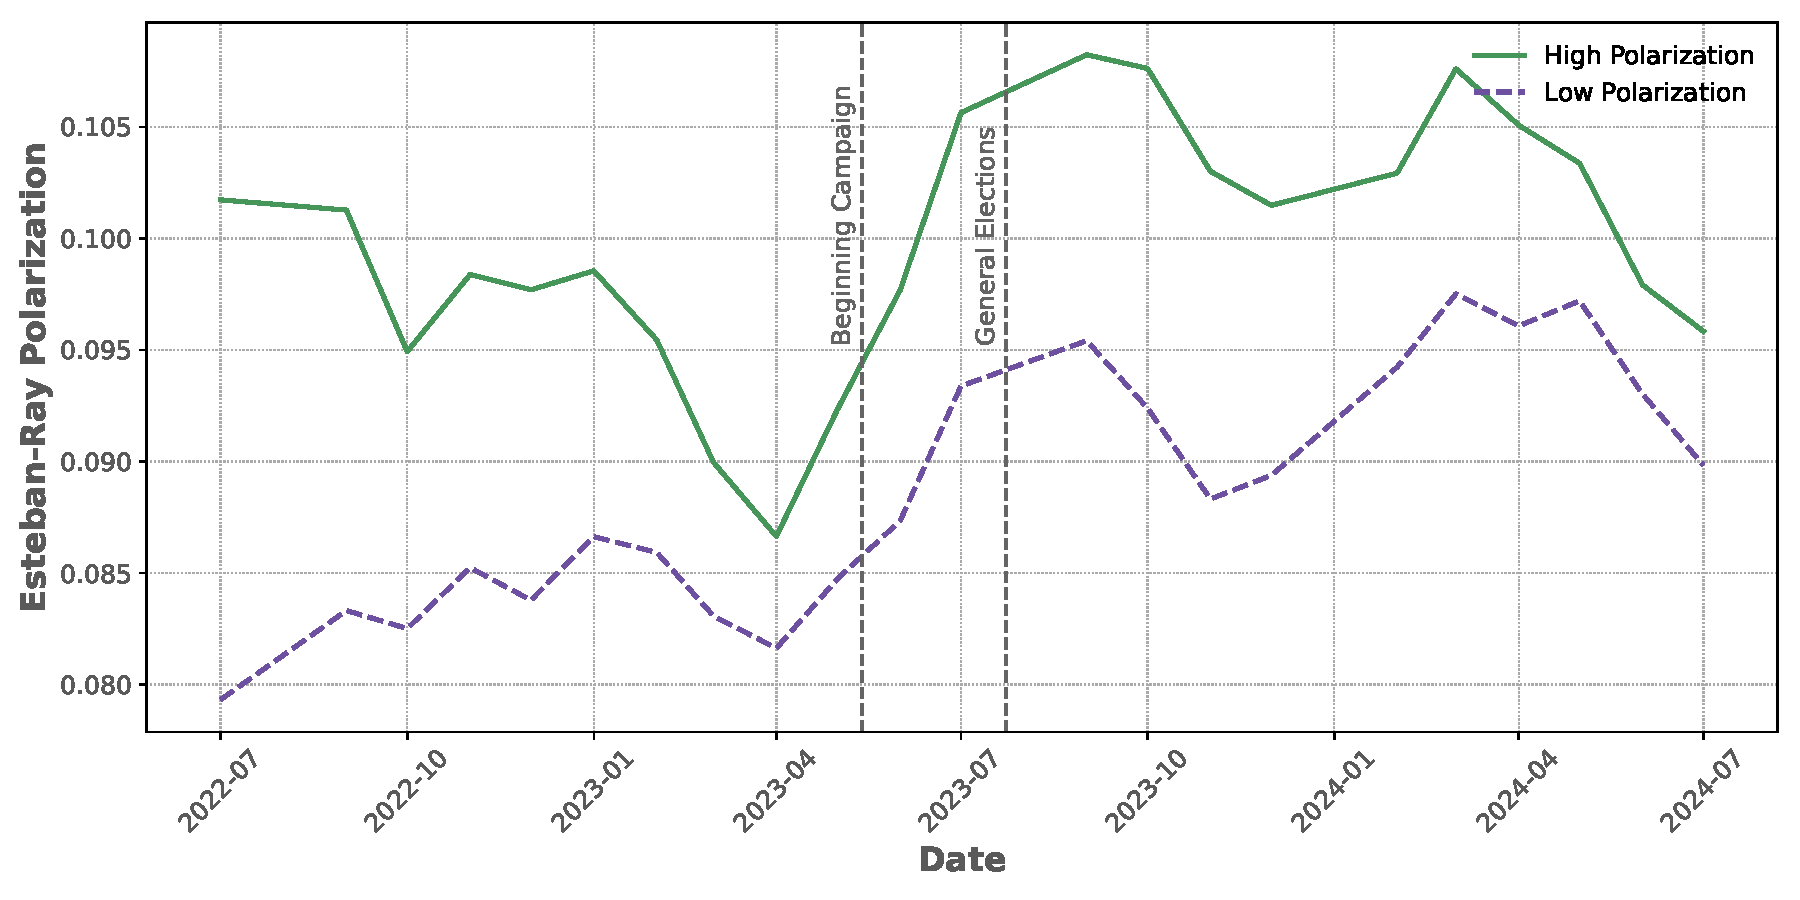
\includegraphics[width=150mm]{figures/er_polarization_stata_group}
				\label{fig:er1}
	\caption*{\textit{Note:} \small The figure shows the mean Esteban-Ray polarization index under a smoothed rolling mean of 3 months computed as in equation \ref{eq:er}.  Solid (dashed) line represents the regions above (below) the median in terms of their media polarization consumption according to index \ref{eq:mediapol}.   }

\end{figure}

 In order to check weather political polarization is driving the results of the demand estimation; I run my model in \ref{eq:utility} using the initial (i.e December) rather than the monthly ideology. Results are robust.  However, the use of aggregate data cannot rule out selection effects. Campaigns might change audience composition towards news seekers, who have been shown to have asymmetric effects relative to entertainment seekers in terms of polarization \citep{levendusky,arceneaux_johnson_2013}. Future work might address this concern with the use of individual panel data or allowing more flexible dynamics between ideology and media consumption as in \cite{martin2017}.




\section{Supply Side}


\label{sec:supply}

News directors explicitly link editorial choices to real-time audience figures:

\begin{quote}
	“Even a news programme is deeply subject to the day-to-day swings of audience share.  
	A drop of half a point when covering a topic can lead us to drop that topic altogether.”
\end{quote}
\hspace*{\fill}\small–––Vicente Vallés, Director and Presenter, Antena 3 News (2014)\footnote{Source: \url{https://cadenaser.com/ser/2014/12/03/television/1417630810_539829.html}}

Two facts follow from this quote. First, although the newscast contains no adverts, outlets maximise the audience they hand over to subsequent slots. Second, editorial decisions are taken at high frequency: producers meet before the \emph{midday} and \emph{evening} editions and update slant in response to fresh stories and the latest ratings.


For channel $j$ on day $d$ and edition $h\in\{0\text{ (mid-day)},1\text{ (evening)}\}$ the problem is



\begin{equation}\label{eq:payoffs}
	\begin{aligned}
		\max_{\{\mathbf{x}_{jdh}\}}   & \left\{   \sum_{r}\bm{s}_{jrd+1}(\bm{x}_{jdh}, \bm{x}_{-jdh})\frac{L_r}{L} -  \mathcal{C}\left(  \bm{x}_{jdh},\bm{z}_{dh}, \bm{\omega}_{jdh}; \bm{\lambda_j}   \right)    \right\}\\
		s.t.   \quad &   x_{jdh}^{L+} +x_{jdh}^{R+} + x_{jdh}^{L-} + x_{jdh}^{R-} + x_{jdh}^{\emptyset} = x_{jdh}^{political}\\
		& x_{jdh}^k \in [0,1] \quad \forall k
	\end{aligned}
\end{equation} 






where $\bm z_{dh}$ measures the pool of stories available at edition~$h$.  
I parameterize the cost function as

\begin{equation*}\label{}
	\begin{aligned}
		& \mathcal{C}(x_{jdh}^k,z_{dh}^k,\omega^k{jdh}; \lambda_j^k )\equiv   \lambda_j^k  \dfrac{(x_{jdh}^k)^2}{z_{dh}^k} + F(\omega^k_{jdh})
	\end{aligned}
\end{equation*} 

where there is a channel-characteristic specific parameter that governs the slope of the production cost and unobserved (to the econometriciaan) cost factors other than the stories available; $ F(\omega^k_{jdh})$. By assumption, these unobservables will enter as linear terns in the marginal costs. The sign of~$\lambda_j^k$
is theoretically ambiguous. On the one hand, $z$ might act as a simple input in any production costs. High availability of stories of a given type will make production easier since the journalist need not do much effort to find them. This will imply $ \lambda_j^k>0$. On the other hand, outlets are news aggregators. Having more stories available of a given type might increase the cost of producing them since they would need to process and filter the ones that they prefer. This mechanism is consistent under $ \lambda_j^k<0$.


\subsection*{First-Order Conditions and Endogeneity}

The first-order condition (ignoring the summation constraint for estimation) is
\begin{equation}\label{eq:focs}
	\sum_{r}\frac{\partial s_{jrd+1}}{\partial x_{jdh}^k}\frac{L_r}{L}=	2\lambda_j^k\frac{x_{jdh}^k}{z_{dh}^k} +\underbrace{	\eta_{jd}^k+\nu_{jdh}^k}_{\equiv F'(\omega_{jdh}^k)},
\end{equation}


I decompose the unobserved cost factors into 
$\eta_{jd}^k$, a \emph{persistent, day-specific} marginal-cost shock
(e.g.\ a key reporter is on sick leave, satellite link fails, or legal concerns delay a segment),
and $\nu_{jdh}^k$ is transitory noise. 
Because $\eta_{jd}^k$ influences both marginal cost and the share gradient
$g_{jdh}^k\equiv\sum_{r}\partial s_{jrd+1}/\partial x_{jdh}^k\,(L_r/L)$,
$\lambda_j^k$ would be biased in a naive regression: $\E[g_{jdh}^k\,\eta_{jd}^k]\neq0$.


The key identification strategy is that $\eta_{jd}^k$ is constant within the day. This allows me to rely on variation in news production within day that is only due to new stories coming in between the midday and evening editions that alter production.  To show the variation that I will exploit, I first regress the evening on the midday editions controlling for outlet fixed-effects. The residuals of these regression are the  variation in the evening programming not explained by the midday slant and channel specific attributes. I then regress these residuals on the stories that enter between those two time slots in EFE. Figure \ref{fig:diff} shows the scatter of the regression. 

There is a positive association for all content categories. This indicates that entry of new content between midday and night is associated with an increase in editorial production of that content in the evening news' shows. 


\begin{figure}[ht!]
		\caption{Within day increase in news production}
	\centering
	\begin{tabular}{@{}cc@{}}
		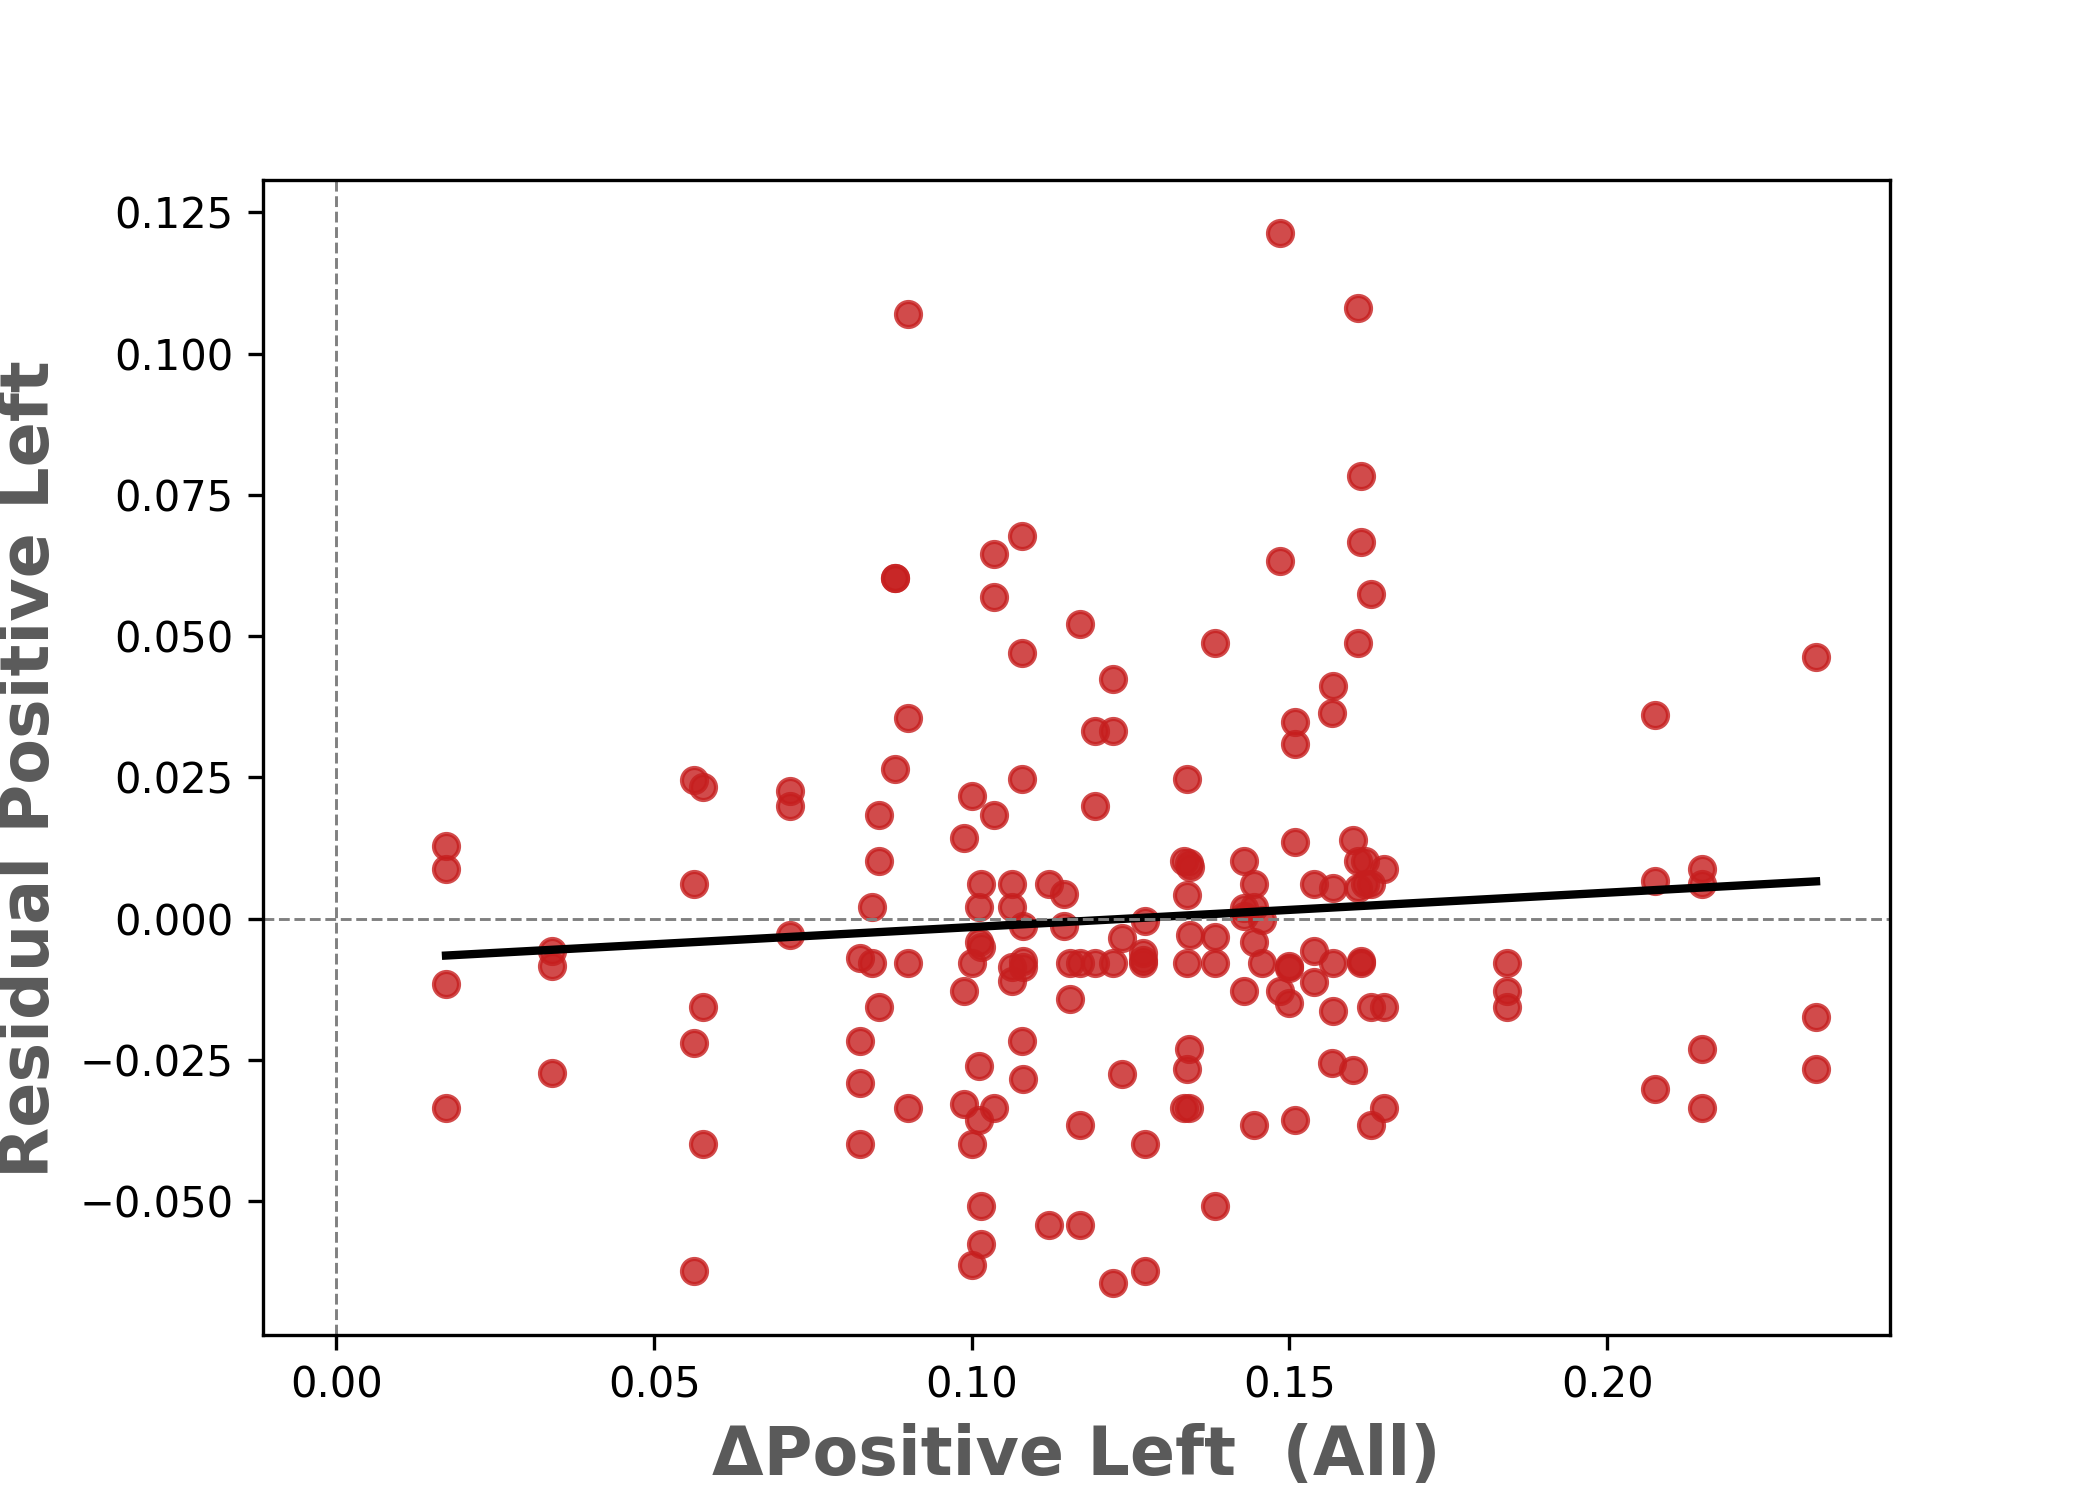
\includegraphics[width=0.5\textwidth]{figures/char_pos_left_residual} &
		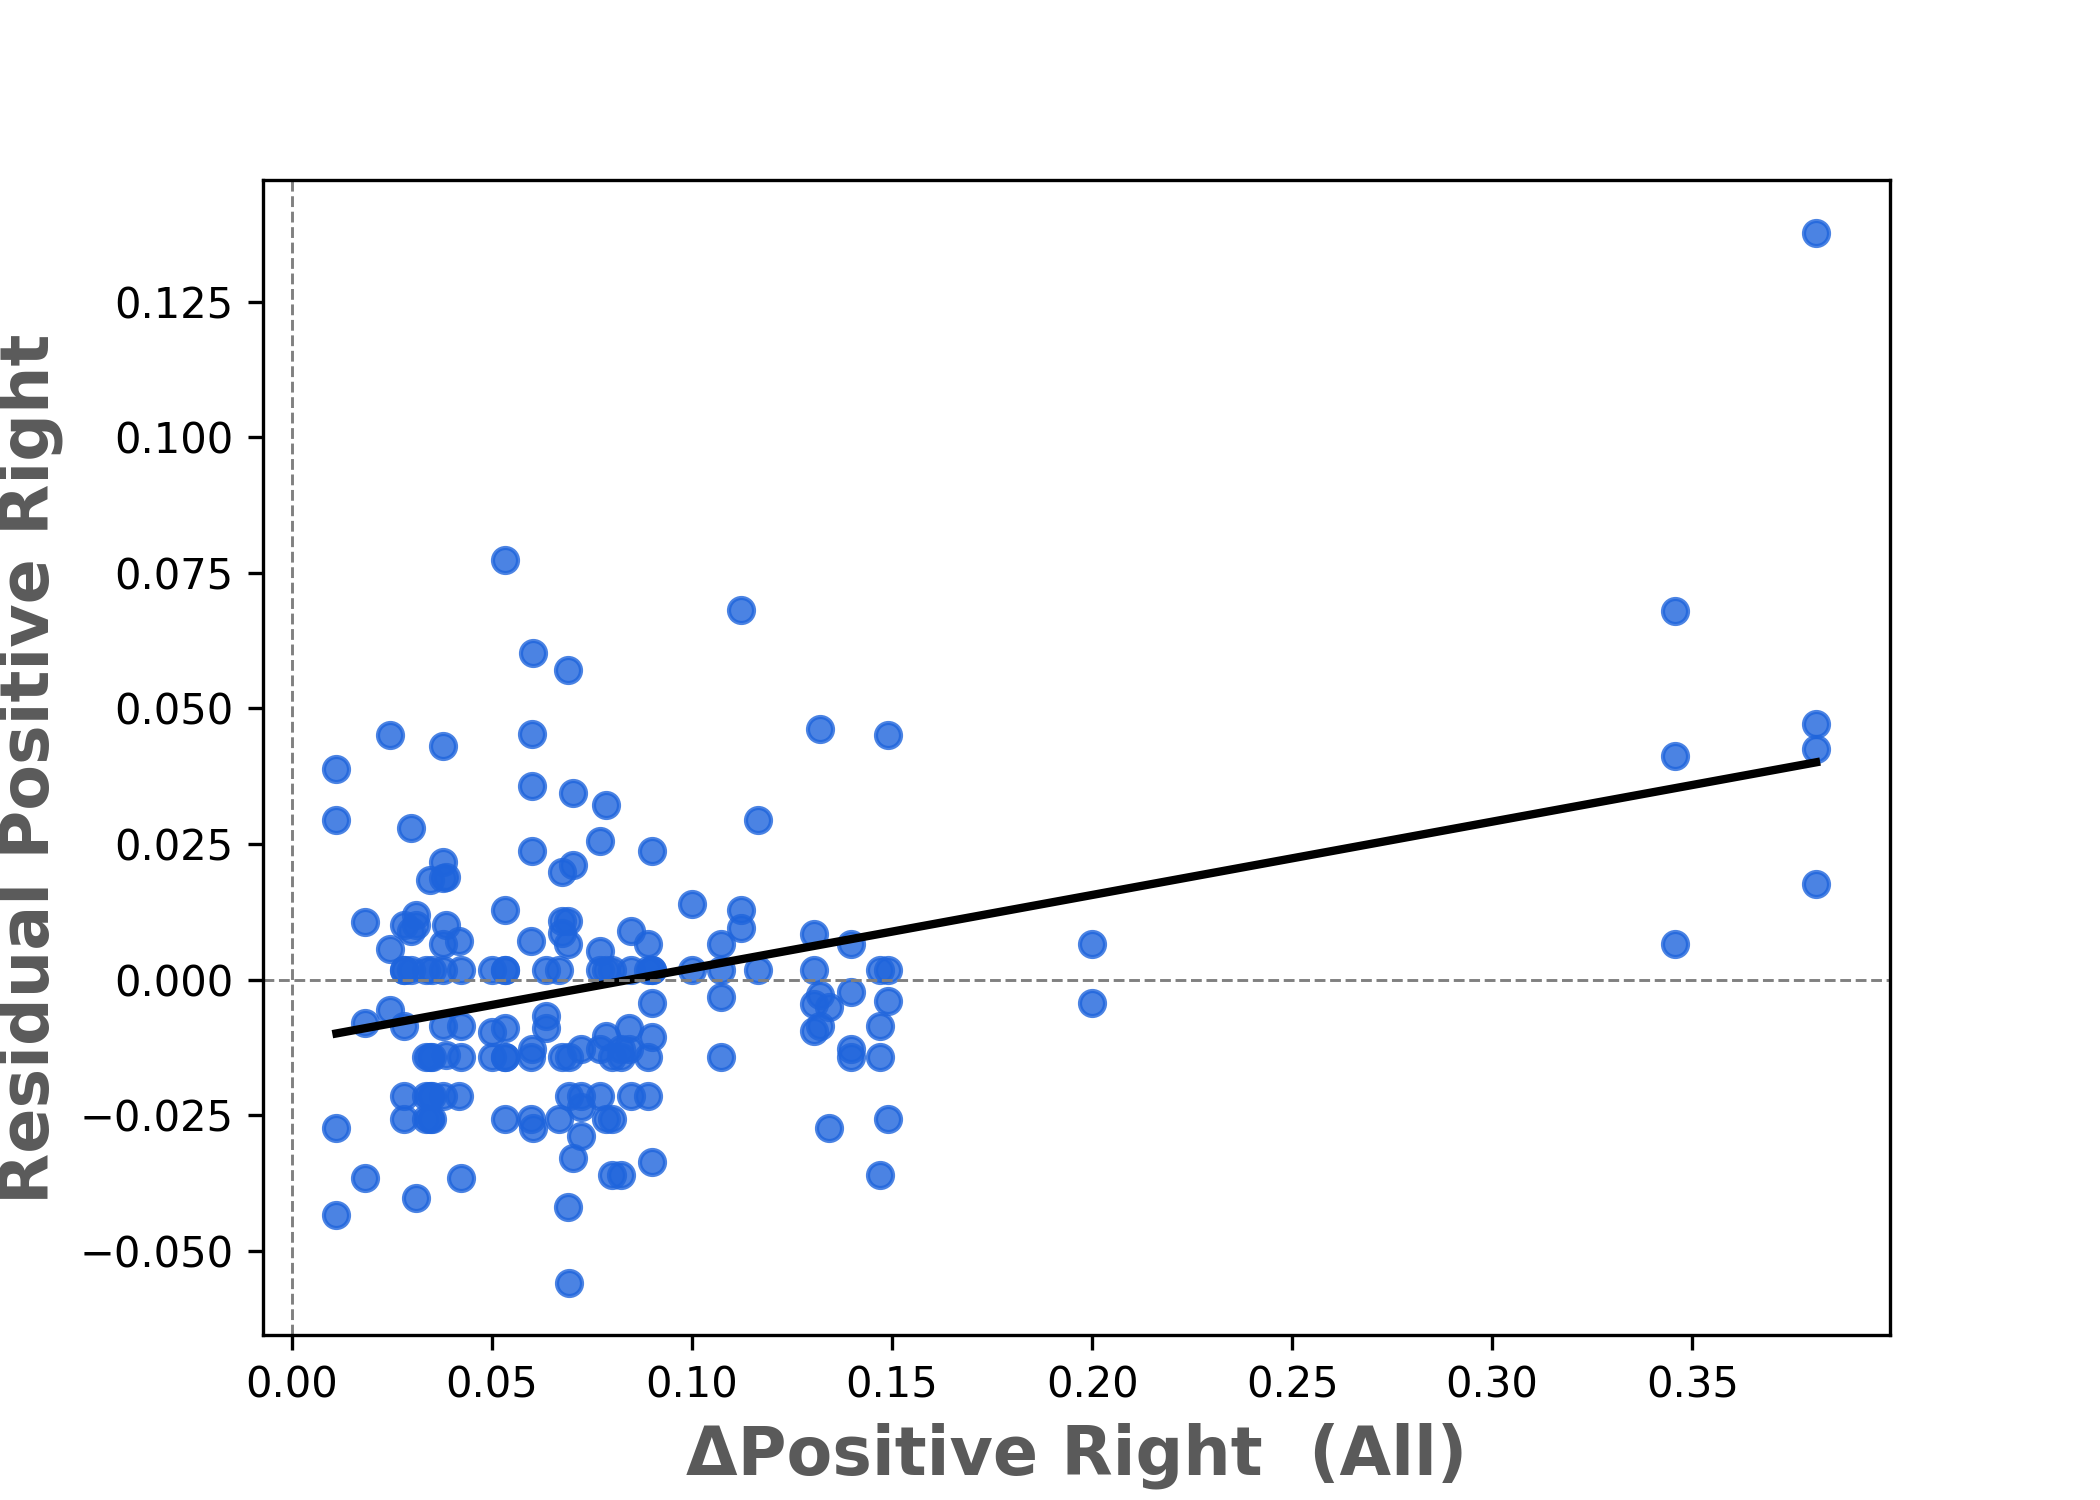
\includegraphics[width=0.5\textwidth]{figures/char_pos_right_residual} \\[-.2pt]
		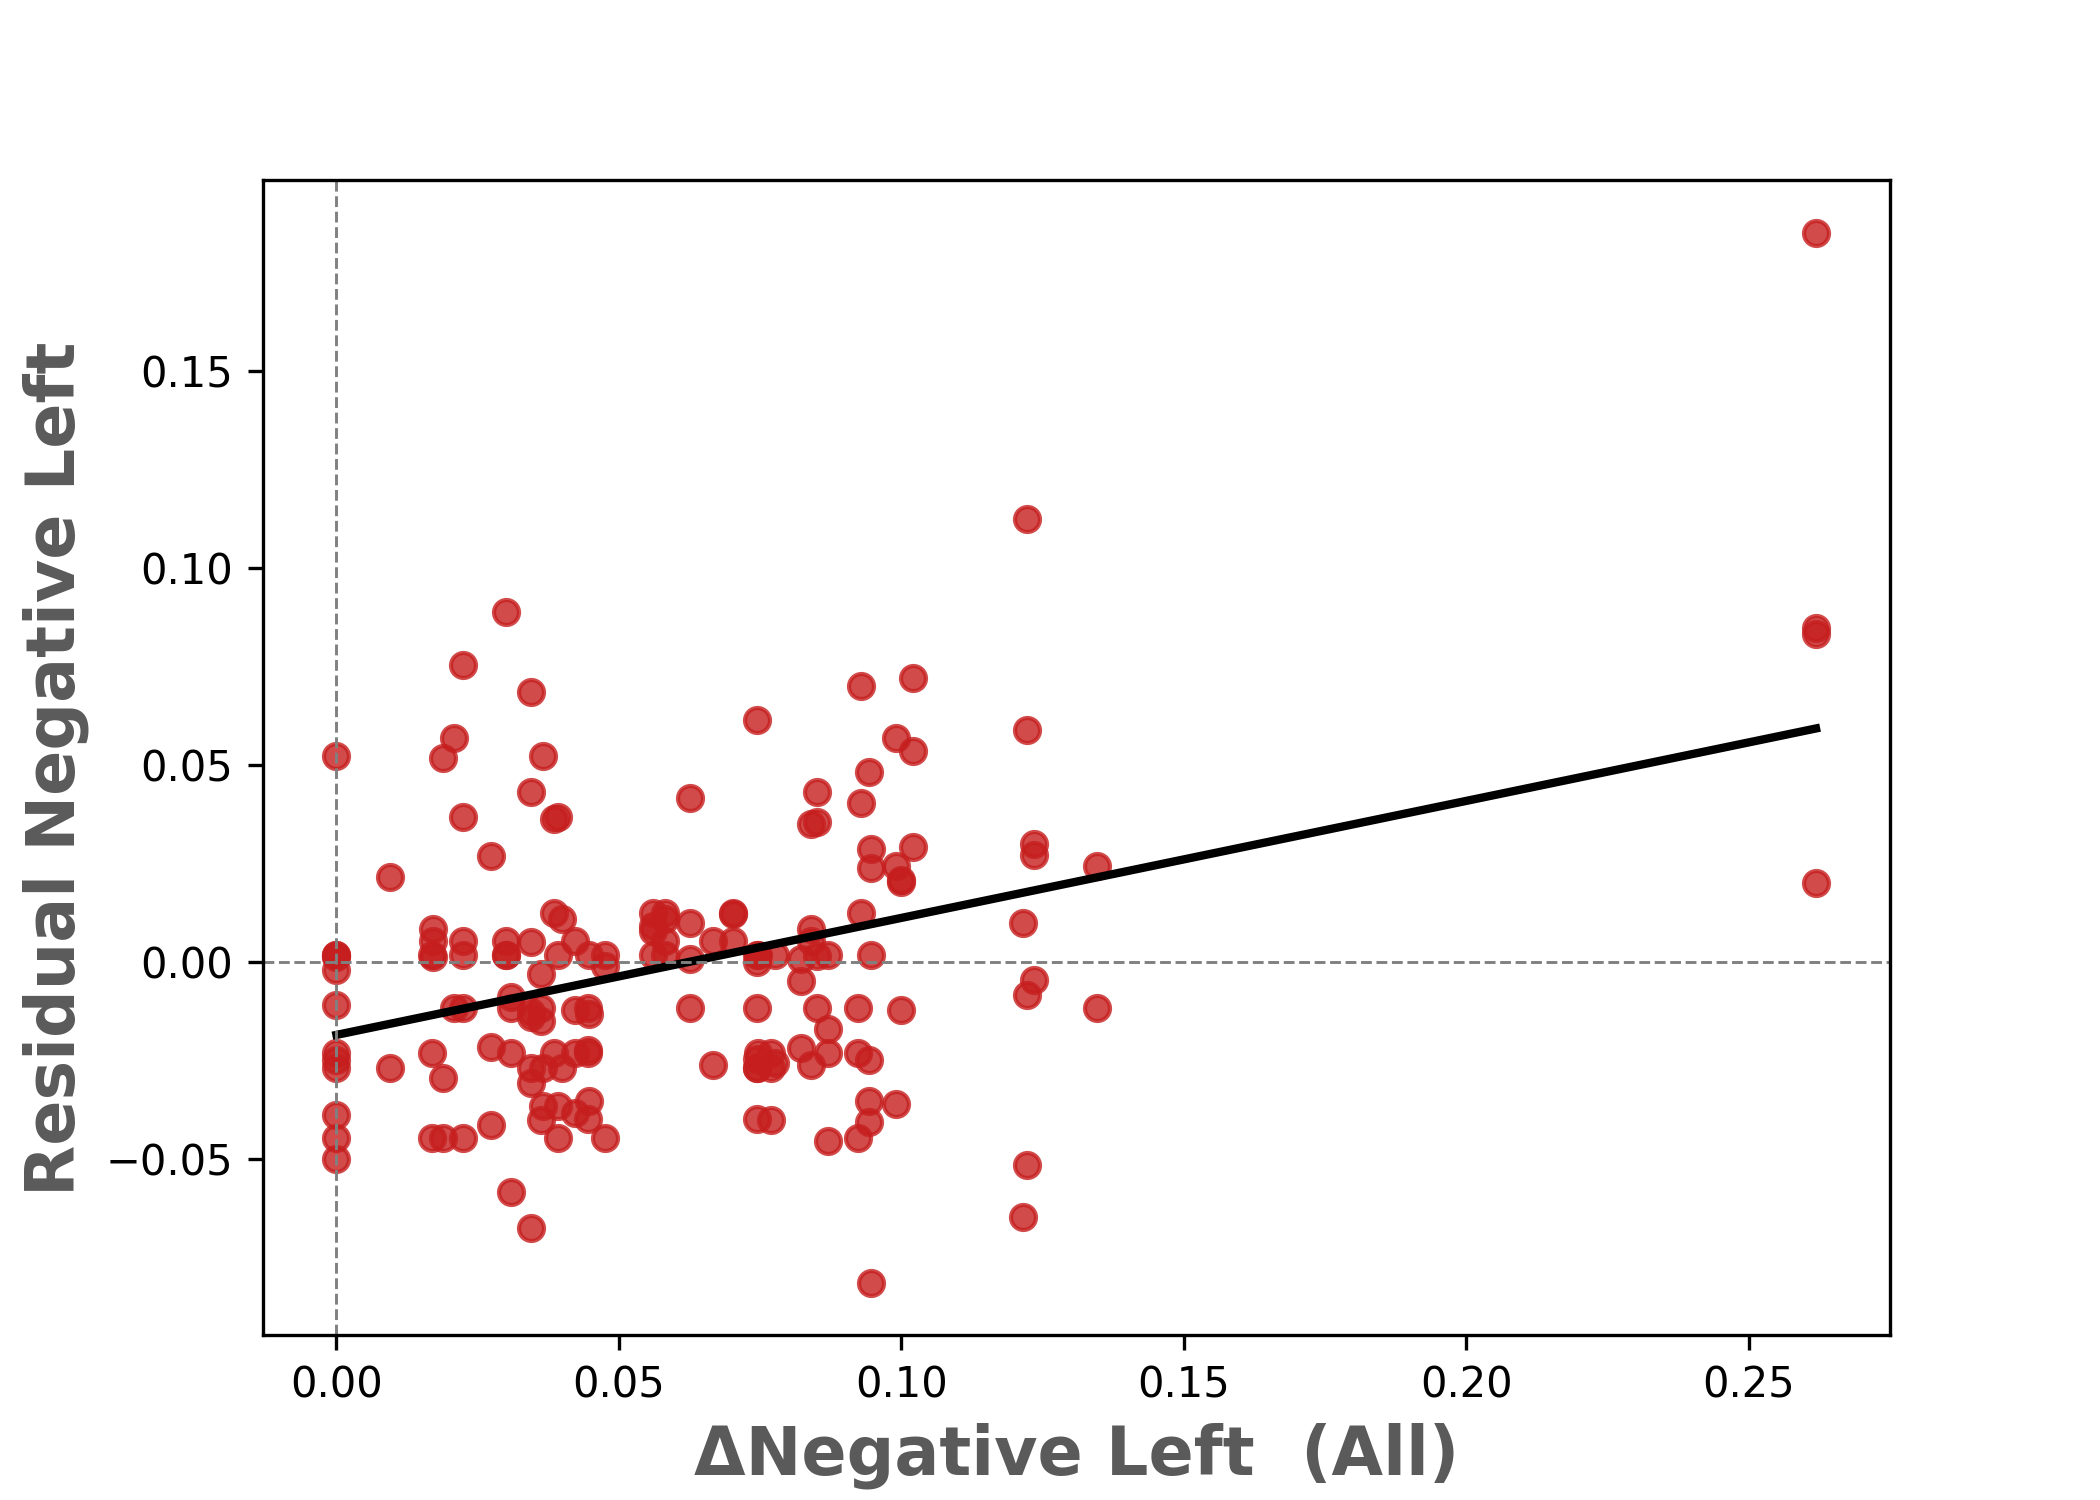
\includegraphics[width=0.5\textwidth]{figures/char_neg_left_residual} &
		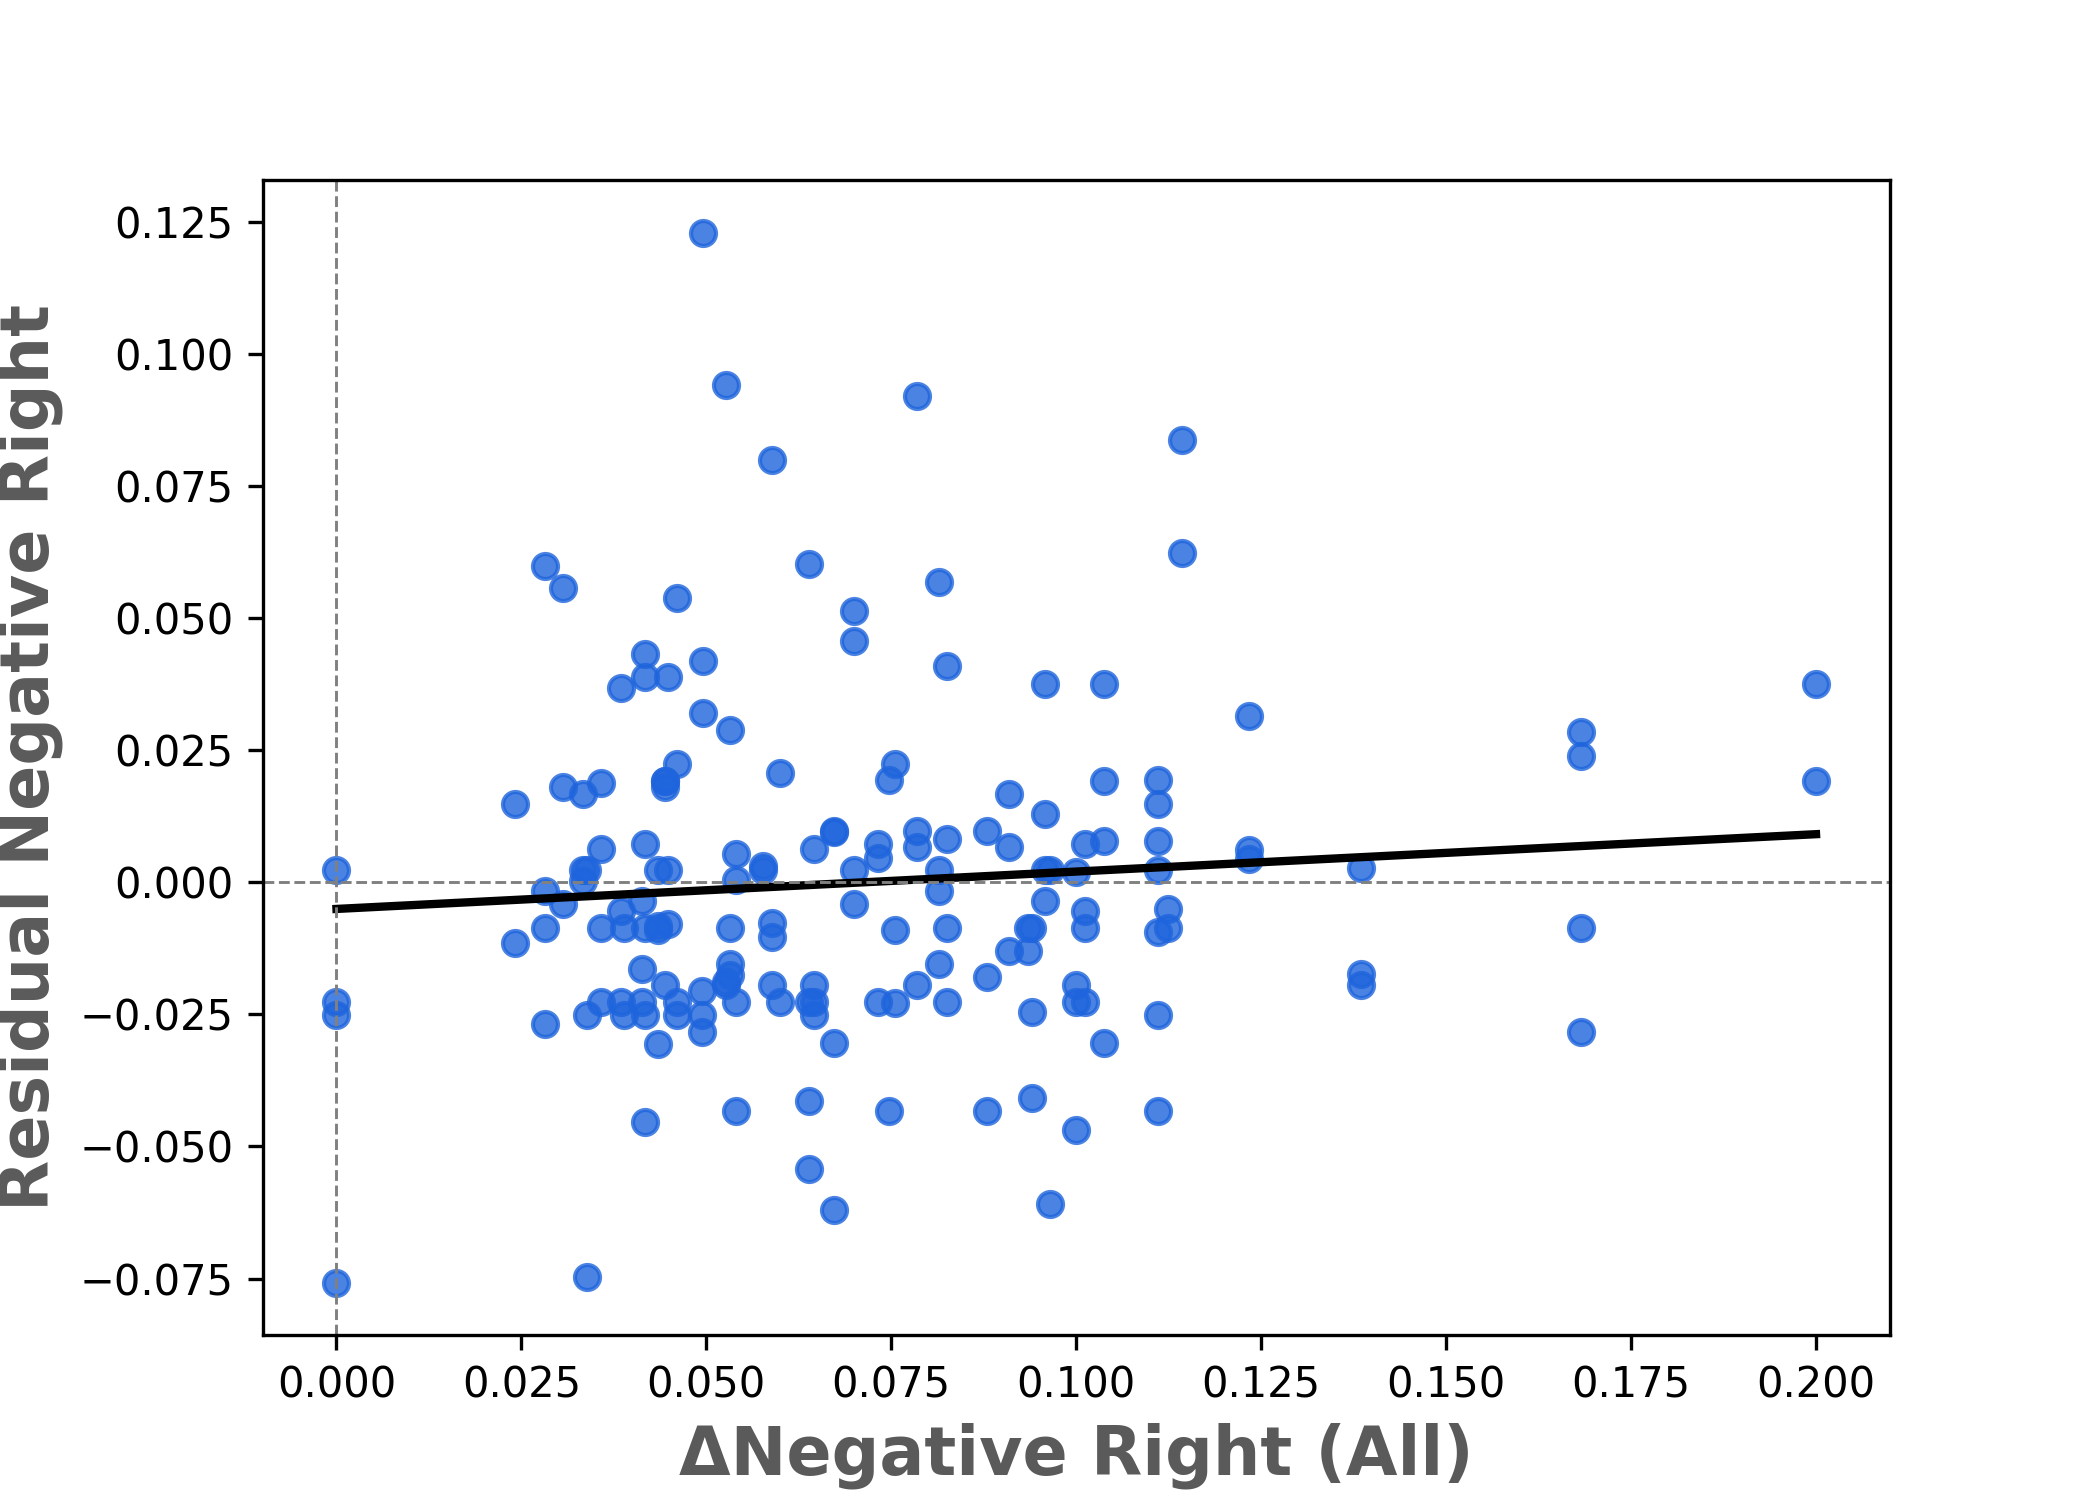
\includegraphics[width=0.5\textwidth]{figures/char_neg_right_residual}
	\end{tabular}
	\caption*{\textit{Note}: \small Scatter with fitted line from the regression of the residual from a regression of the evening tone on the midday tone with outlet fixed effects on the tone of the stories in EFE between midday and evening.}

	\label{fig:diff}
\end{figure}


To decompose this variation by outlet, I run regressions of the form \ref{eq:first_stage} done on within day differences $ \Delta x_{jd}$ and $\Delta z_{d}$. Figure \ref{fig:fwl_diff} on the appendix shows the added variable plots. Although there is significantly less power now, the main mechanism still holds. Right (left) outlets increase more their production of stories of a given party-tone from midday to the evening editions conditional on those stories being aligned with their stances. 



 Table \ref{tab:within} shows examples on the text. I filter the days with the highest within-day increase in coverage by all channels and report the new stories that entered between midday and evening editions for each content type. For instance, nn 29 May 2023, stories criticizing the left pushed evening coverage sharply toward a pro-right tone; on 31 May 2023, stories criticizing the right swung coverage the opposite way. These sudden, within-day shifts in story mix create the variation we use to measure viewers’ taste for like-minded versus opposing content.










Differencing~\eqref{eq:focs} eliminates the unobserved shock:
\begin{equation}\label{eq:diff_foc}
	\underbrace{%
		\sum_{r}\left(
		\frac{\partial s_{jrd+1}}{\partial x_{jd1}^k}
		-
		\frac{\partial s_{jrd+1}}{\partial x_{jd0}^k}
		\right)\frac{L_r}{L}
	}_{\Delta g_{jd}^k}
	\;=\;
	2\lambda_j^k
	\left(
	\frac{x_{jd1}^k-x_{jd0}^k}{\,z_{d1}^k-z_{d0}^k}
	\right)
	\;+\;
	\Delta\nu_{jd}^k.
\end{equation}
Intuitively, the evening–mid-day change in the gradient, $\Delta g_{jd}^k$, is driven by the change in story availability $(z_{d1}^k-z_{d0}^k)$, while the day-persistent cost shock cancels out.



\subsection{Results}





Table~\ref{table:costs} reports the estimated $\lambda_j^k$ \footnote{Due to computational issues with the pre-processing of the midday shows for the pre-campaign period; this section presents the cost estimation only for the campaign period. }.  
Producing content favourable to the left (positive-L or negative-R)
is costlier for the right-leaning Antena~3,
while the reverse holds for left-leaning La~Sexta and TVE.  
Telecinco, a centrist outlet, faces the lowest absolute costs in every category.




\begin{table}[H]
	\caption{Estimated Cost Parameters ($\lambda$) by Channel and Content Type}
	\label{table:costs}
	\centering\small
	\begin{tabular}{lcccc}
		\toprule
		& La~Sexta & TVE & Telecinco & Antena~3 \\
		\midrule
		% Group 1
		Negative Left   
		& 12.782   &  6.614   & 108.985   & --38.135  \\
		& (44.512) & (3.107)  & (60.695)  & (24.006)  \\
				\midrule
		Positive Right  
		& --89.175 & --105.658 & --13.868  & --238.018 \\
		& (85.860) & (121.713) & (91.624)  & (77.314)  \\
		\midrule
		% Group 2
		Positive Left   
		& 36.094   &  3.368   &  25.984   & --38.962  \\
		& (52.716) & (13.110) & (43.586)  & (84.390)  \\
				\midrule
		Negative Right  
		&  4.059   & --8.694  &  30.280   &  34.624   \\
		& (4.788)  & (11.057) & (36.013)  & (53.835)  \\
		\midrule
		% Group 3
		Political 
		& --0.349  &  0.317   &   1.498   &   1.455   \\
		& (0.610)  & (0.622)  &  (1.049)  &  (1.248)  \\
		\bottomrule
	\end{tabular}
	\vspace{0.5em}
	\caption*{\scriptsize\emph{Note:} Robust standard errors in parentheses. Table shows the estimated coefficients under GMM for equation \ref{eq:diff_foc}.}
\end{table}



The signs confirm the interpretation: left-favourable content is costlier for right-leaning outlets, and vice versa for all characteristics but for positive left content. 
These outlet–slant asymmetries feed directly into the counterfactuals in Section~\ref{sec:counter}.



































\section{Counterfactuals: Work in progress}

\label{sec:counter}


Across Europe, broadcast regulators increasingly impose proportional-air-time rules to curb partisan imbalances in election coverage: France’s ARCOM stopwatches every political segment to enforce strict minute-for-minute equality during the “période officielle”; Italy’s Par Condicio law compels both public and private stations to “balance and compare” exposure for all lists; and Germany grants each registered party free television slots whose length scales with its prior vote share. Spain, by contrast, still relies on a voluntary pluralism. The public network TVE issues a proportional airtime manifesto while commercial groups—Atresmedia and Mediaset—entirely unconstrained. 

My model estimates allow to test what would be the implications of enforcing such policy to all the broadcasters.  I take the proportion of votes in the past general elections for each party and estimate the new equilibrium under the following problem: 



\begin{equation}\label{eq:payoffs2}
	\begin{aligned}
		\max_{\{\mathbf{x}_{jd}\}}   & \left\{   \sum_{r}s_{jrd+1}(\bm{x}_{jd}, \bm{x}_{-jd})\frac{L_r}{L} - \sum_k {\lambda_j^k}\mathcal{C}({x}^k_{jd}, {z}^k_d)+ \bm{\eta}_{jd}\bm{x}_{jd} \right\}\\
		s.t.   \quad &   \frac{x_{jd}^{R+} + x_{jd}^{R-} }{x_{jd}^{political}}=vote^R\\
		&  \frac{x_{jd}^{L+} + x_{jd}^{L-} }{x_{jd}^{political}}= vote^L\\
		& x_{jd}^k \geq 0 \quad \forall k
	\end{aligned}
\end{equation} 


where, in a logic consistent with my measurement strategy, time to a political party can only be discerned if that story has some specific slant. I assume that the policy is enforced; that is all outlets must devote the proportion of political time given by previous proportions of votes $(vote^R, vote^L)$ (i.e constraints bind). 



	
	\section{Conclusion}
	
	Understanding the demand of political information is crucial to understand political polarization and media market regulation. However, endogeneity concerns often  impede classical demand estimation techniques due to the lack of valid instruments. In this paper,  I introduce a novel dataset that comprises the Spanish TV market, where I match daily transcripts of the TV news to audimeter data on viewership. I propose a new methodology that makes uses of text analysis and Large Language Models (LLMS ) to analyze the production of political content in TV news. This methodology extracts the political tone and intensity of the daily TV news and  exploits the random availability of political events, together with channel's long-run ideological positions, to measure supply shocks that allow the estimation of  demand preferences.
	
	I show that channels face asymmetric constraints  in their production of political content depending on whether the composition of the day is more or less favorable to their ideological stance. I estimate a structural BLP demand model where I split my sample into both pre-campaign and during political campaign periods. This model allows me to introduce heterogeneity into the demand estimation and decompose political preferences based on the  ideological composition of the audience. My results reveal that while there is no significant asymmetric demand for political content during the pre-campaign period, affective polarization emerges during the political campaign, with right-wing viewers demanding more negative content about the opposing party and more favorable content about their own. Finally, I model the competition game into channels' daily content production and estimate their cost structures. Right wing media enjoy higher benefits/costs on producing content that goes against their editorial line.
	
	
	
	
	
	
	%\nocite{*}
	\clearpage
	%\addcontentsline{toc}{chapter}{Bibliography}
	%\printbibliography
	
	%\addcontentsline{toc}{chapter}{Bibliography}
	\pagestyle{plain}  
	\bibliographystyle{apa}
	
	\bibliography{./bib/media_bias.bib}
	
	
	
	\clearpage

\appendix

\addcontentsline{toc}{section}{Appendix} % Add the appendix text to the document TOC
\part{Appendix} % Start the appendix part

\parttoc % Insert the appendix TOC


\renewcommand\thefigure{\thesection.\arabic{figure}}   
\renewcommand\thetable{\thesection.\arabic{table}}
\setcounter{table}{0}


\clearpage

\section{Figures}
	
	
	

	
	\begin{figure}[!htb]
		\centering
		\caption{Pipeline for content downloading and classification }
		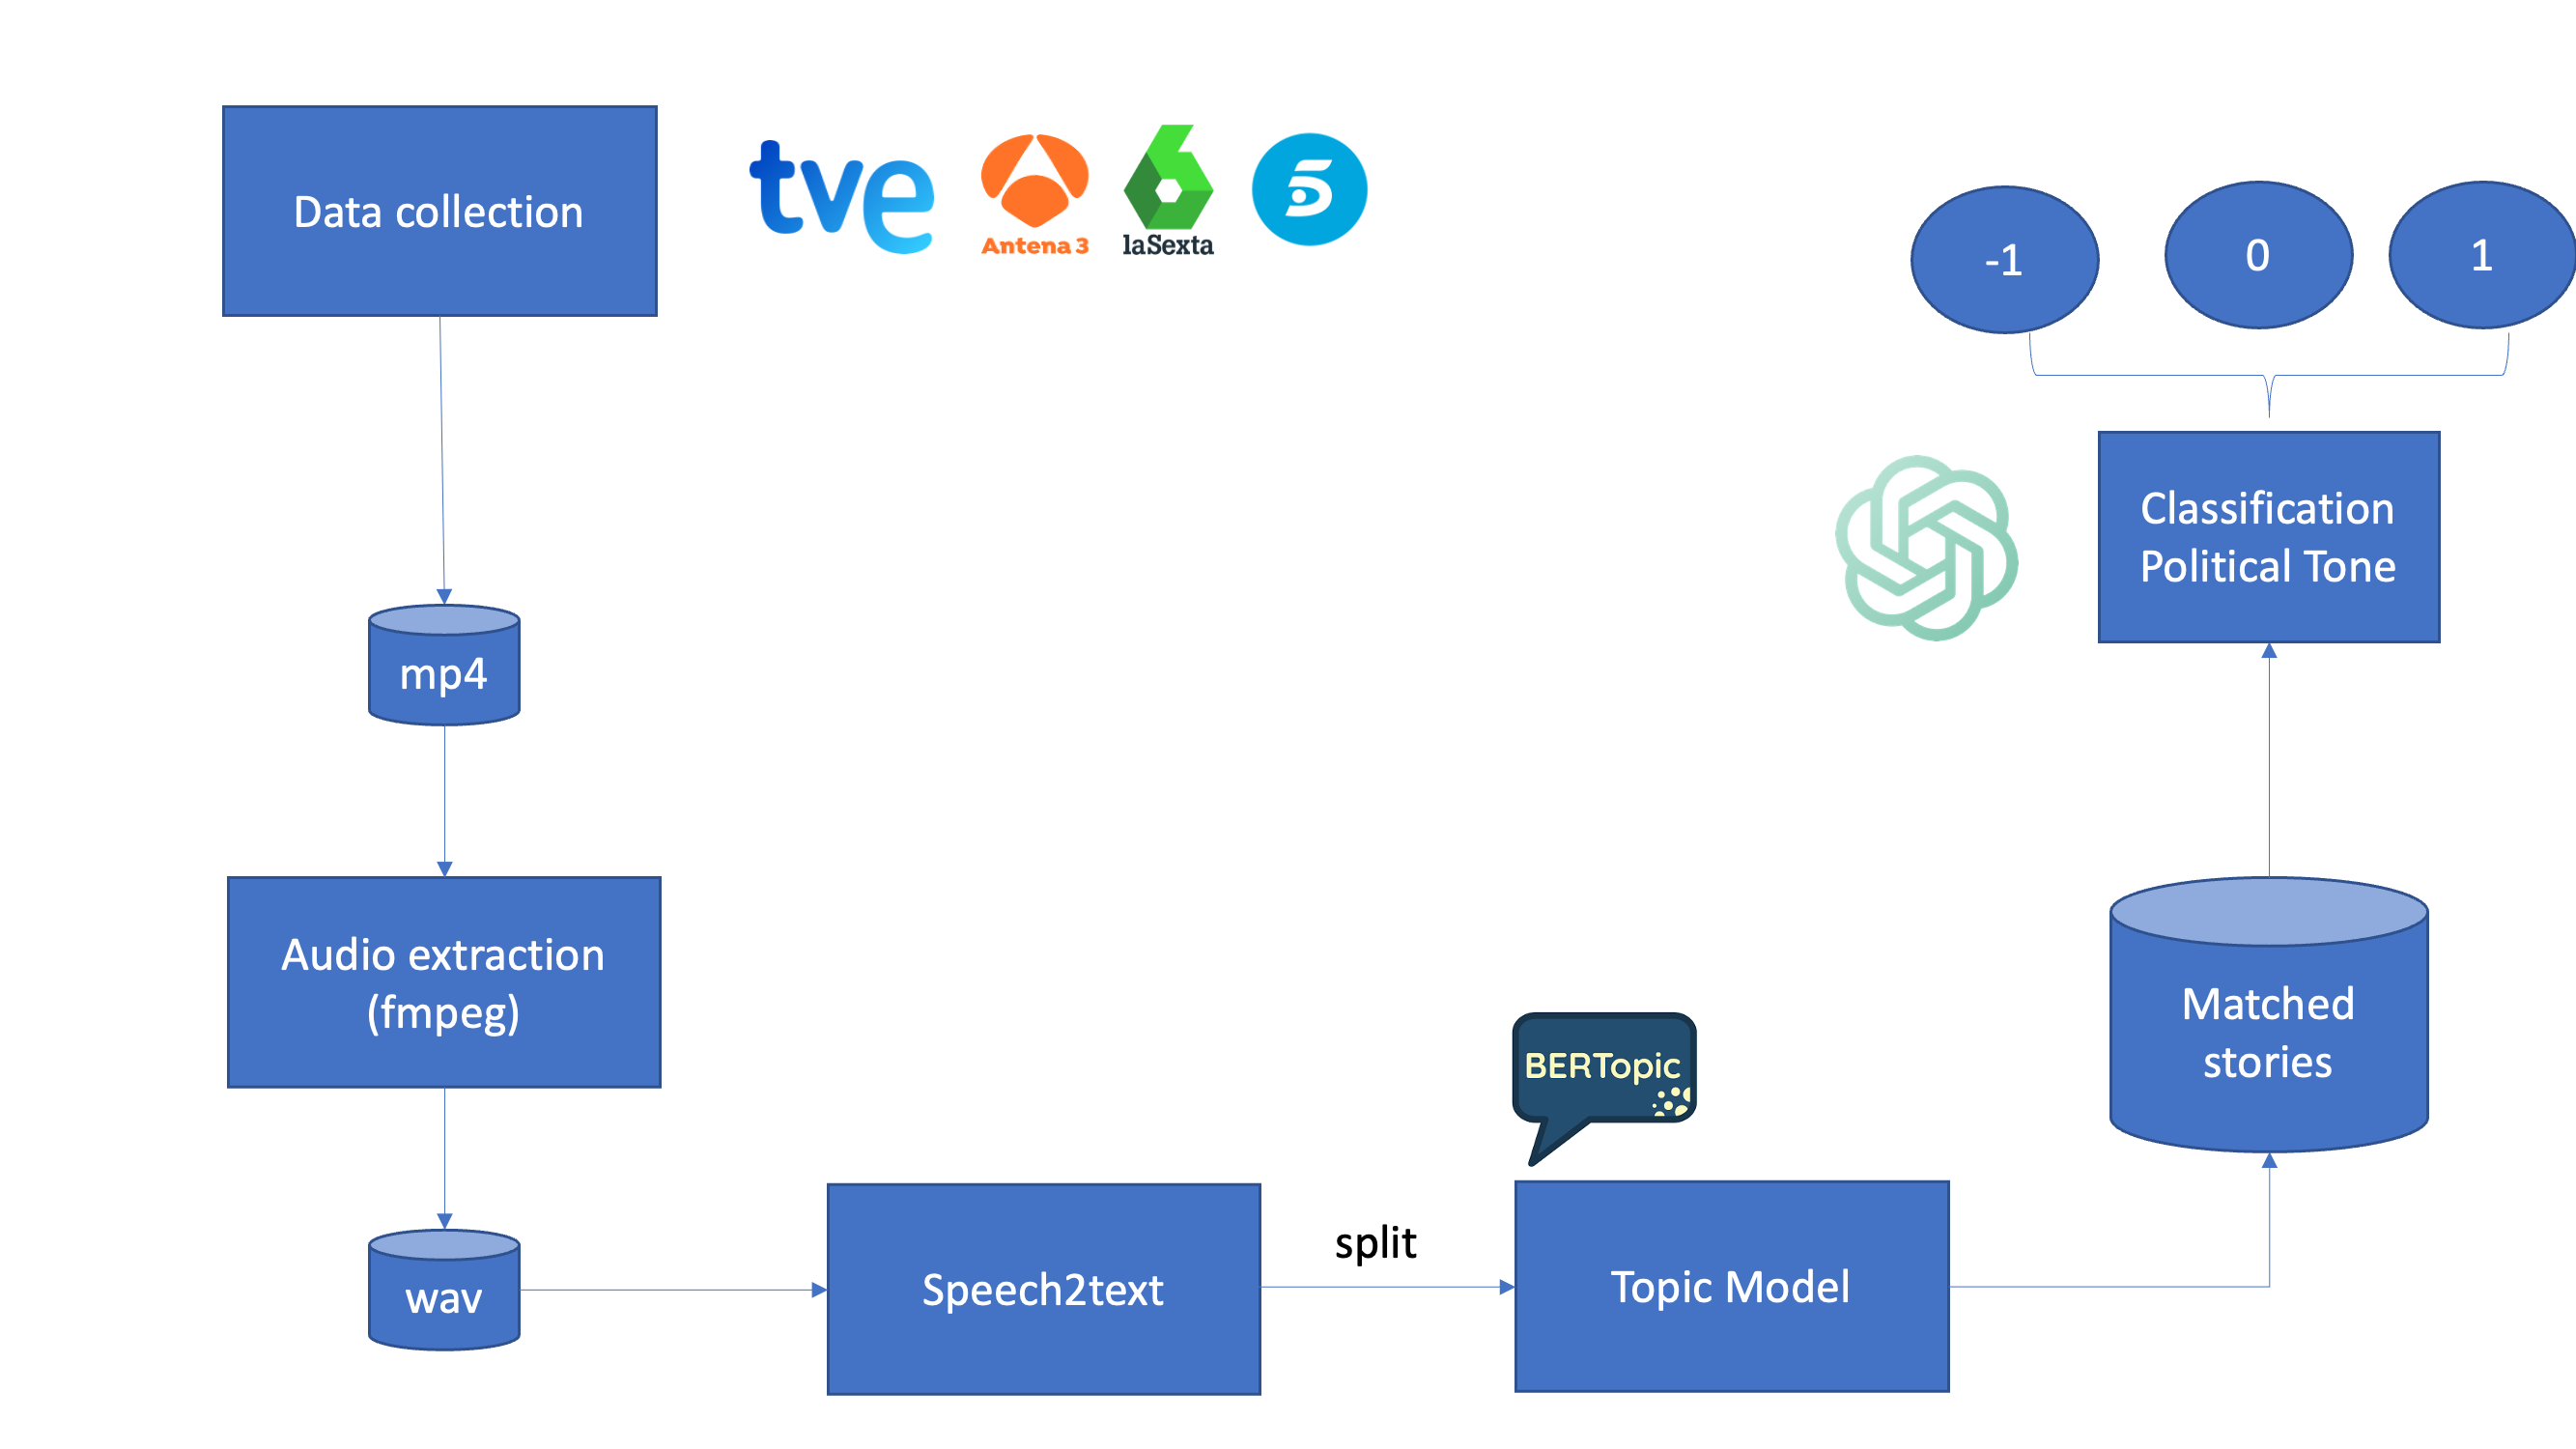
\includegraphics[width=150mm]{figures/pipeline3}
		\caption*{\small Notes: Pipeline for the text downloading. First videos are downloaded daily from the main TV channels. Google engine is used to convert the audio to text. I then split the stories by minute and use BERTopic to classify and match them. Finally, ChatGPT4 is used to classify political tone.}
		\label{fig:pipeline}
	\end{figure}
	
	
	
	
	\begin{figure}[!htb]
		\centering
		\caption{Preferred Media for Political Information in Europe}
		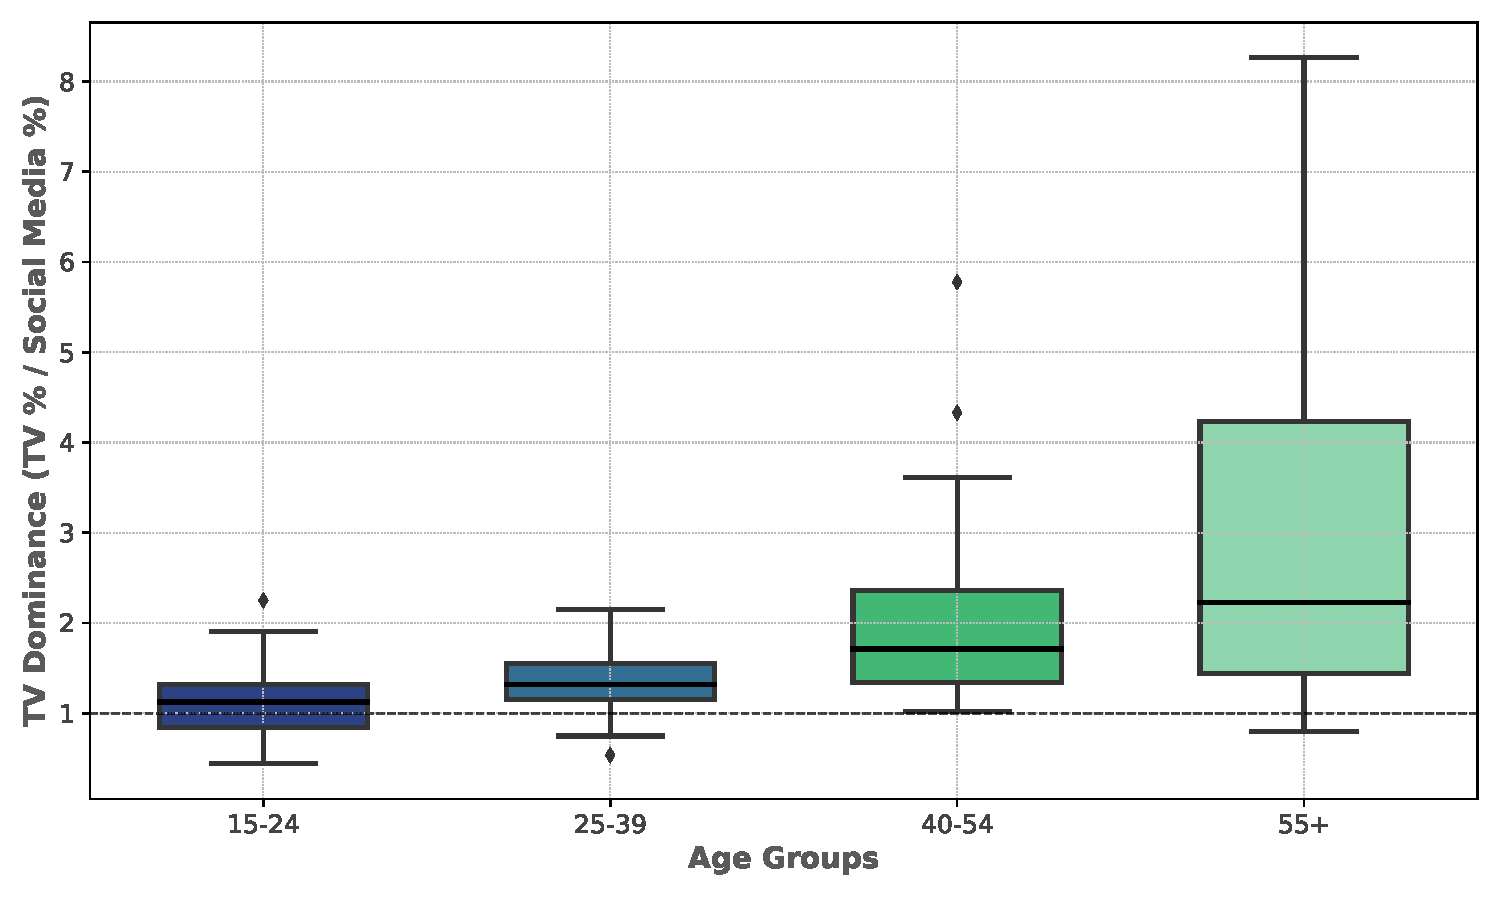
\includegraphics[width=120mm]{figures/age_cohorts_full}
		\caption*{\small Notes: Histogram of the preferred media used for political information in Europe. Using data for the 27 countries in Eurobarometer with $N=112059.$ 
			Source: Eurobarometer, 2022. }
		\label{fig:motivation2}
	\end{figure}
	
	\begin{figure}[!htb]
		\caption{Net sentiment across channels and parties pre and during campaign }
		\centering
		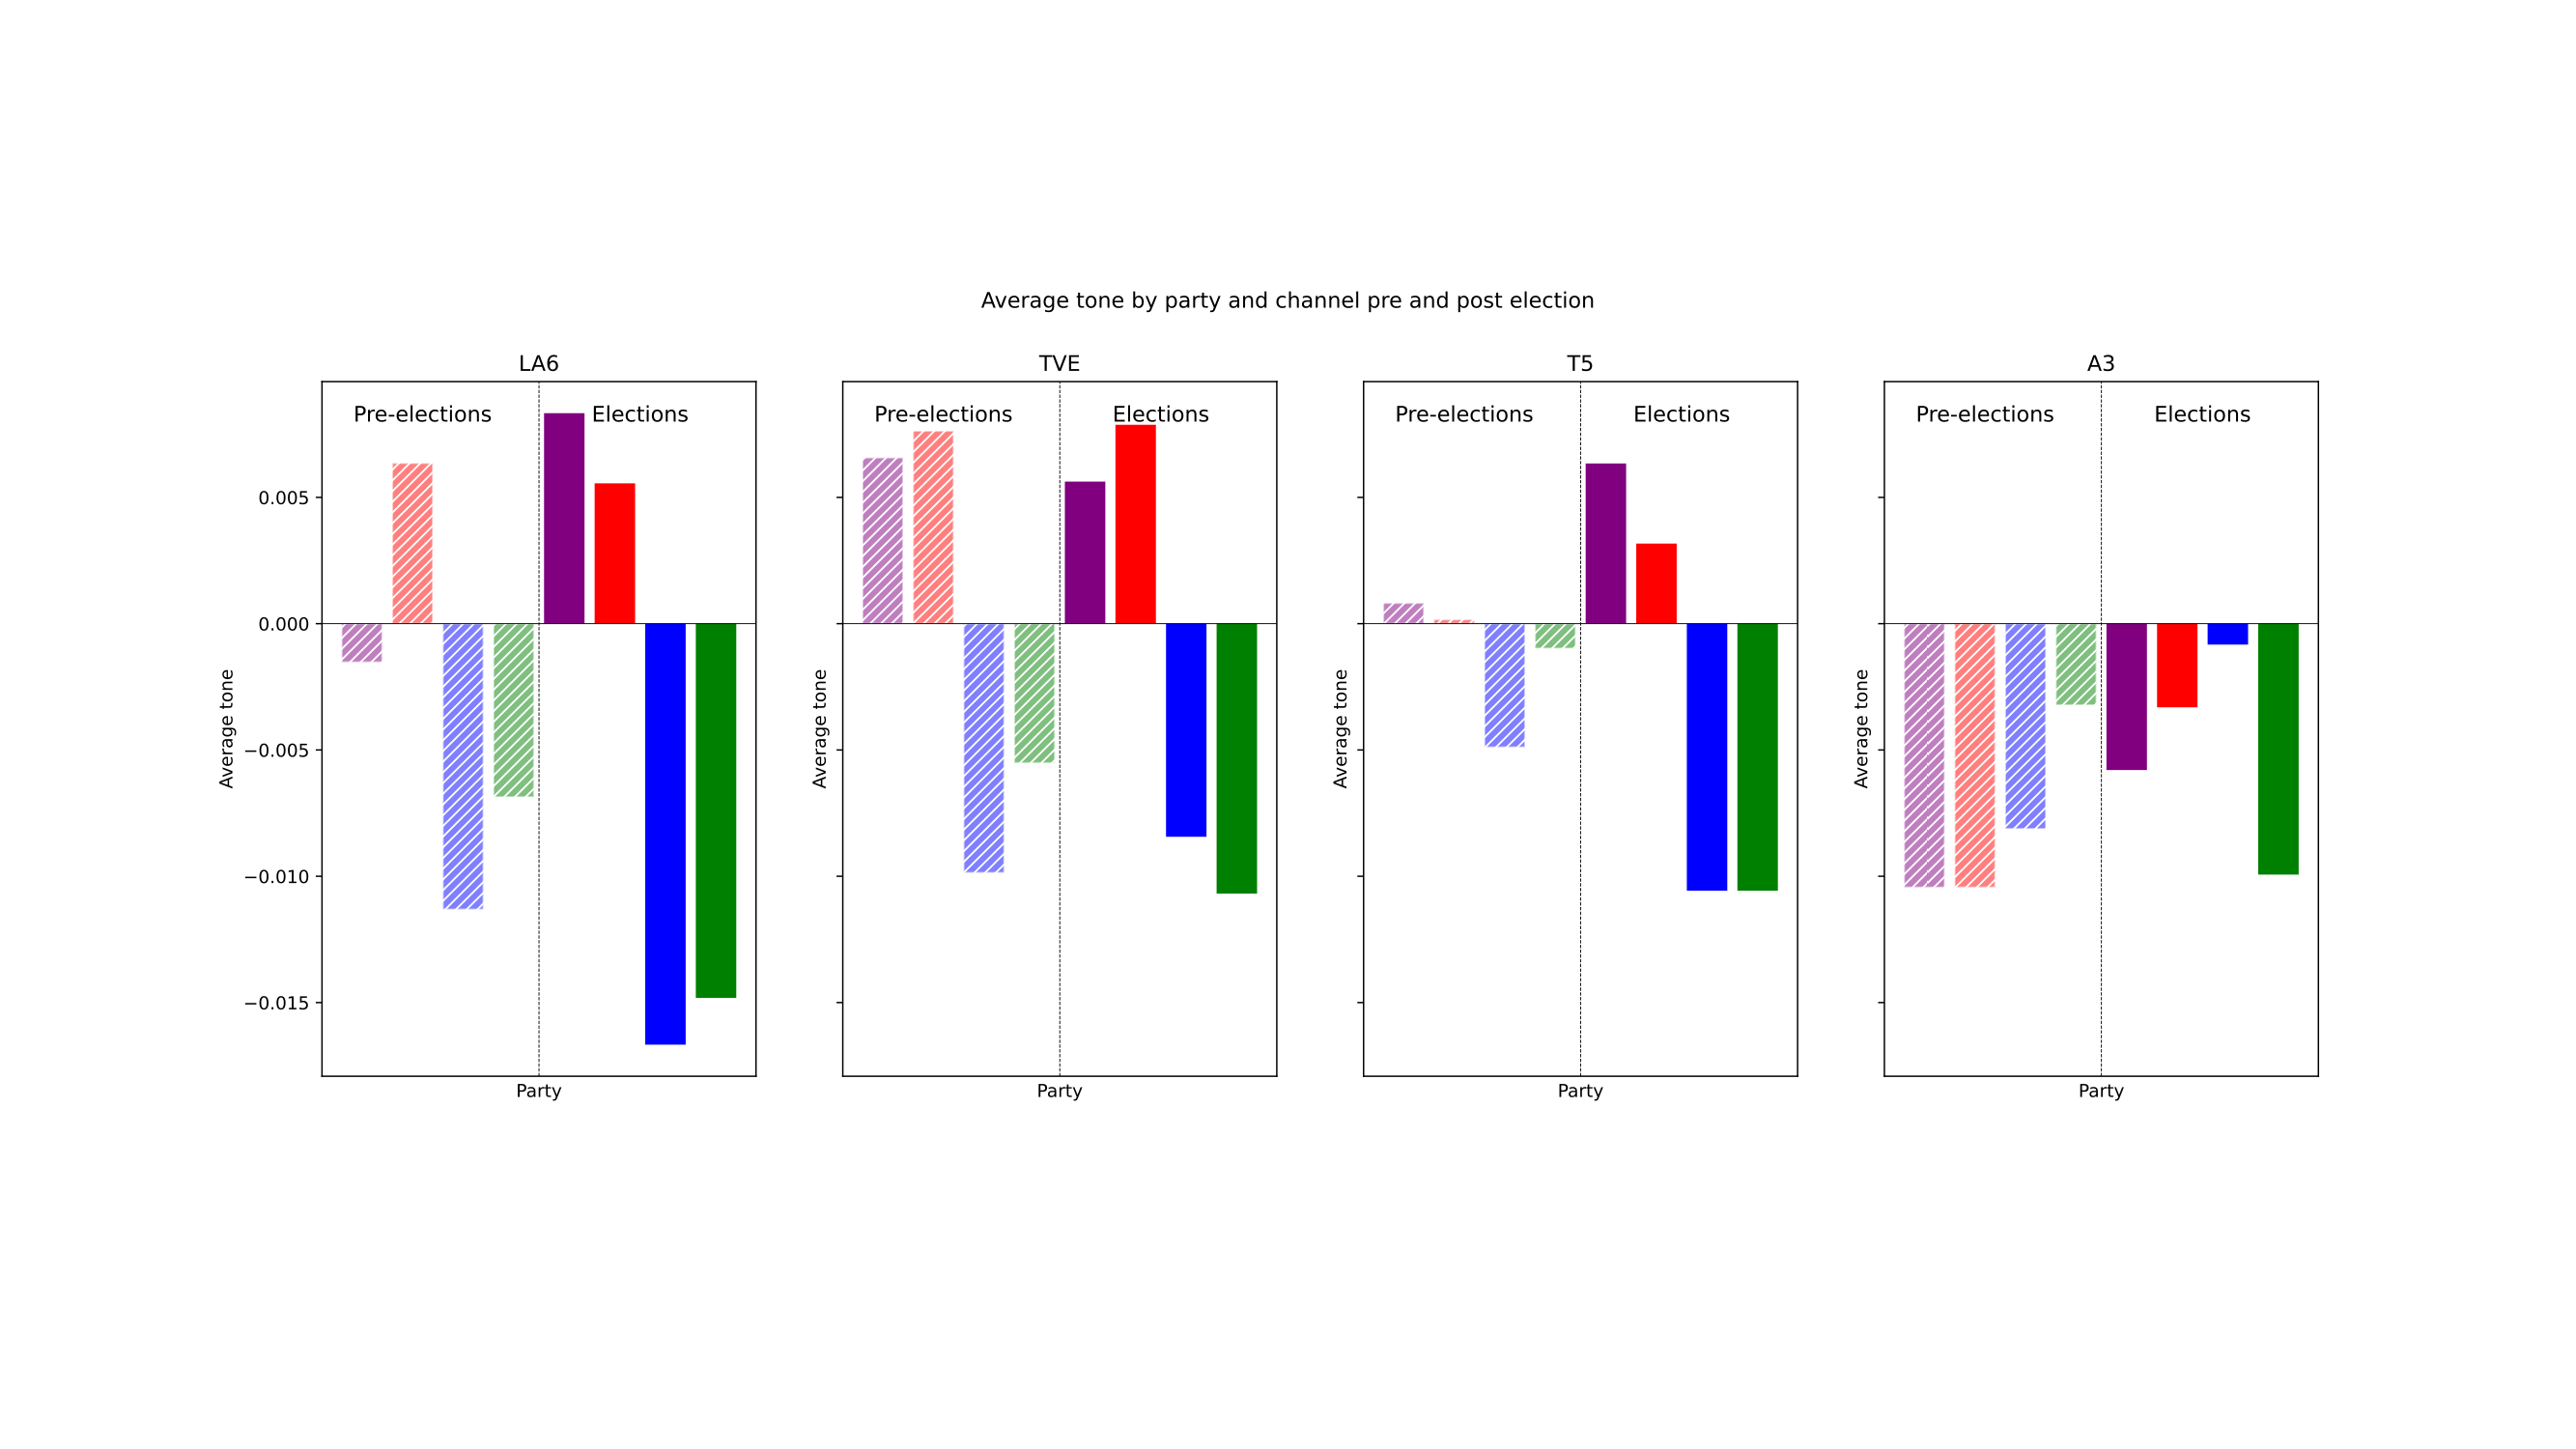
\includegraphics[width=150mm]{figures/average_tone_pre_post_election}
		\caption*{\small Notes: The figure shows the relative tone calculated as the average sentiment over right and left parties. The vertical dashed line delimits results pre and during campaign periods, respectively. }
		\label{fig:tone2}
	\end{figure}
	
	
	
	
		\begin{figure}[!htb]
		\caption{Proportion of Image appearances per channel and politician}
		\centering
		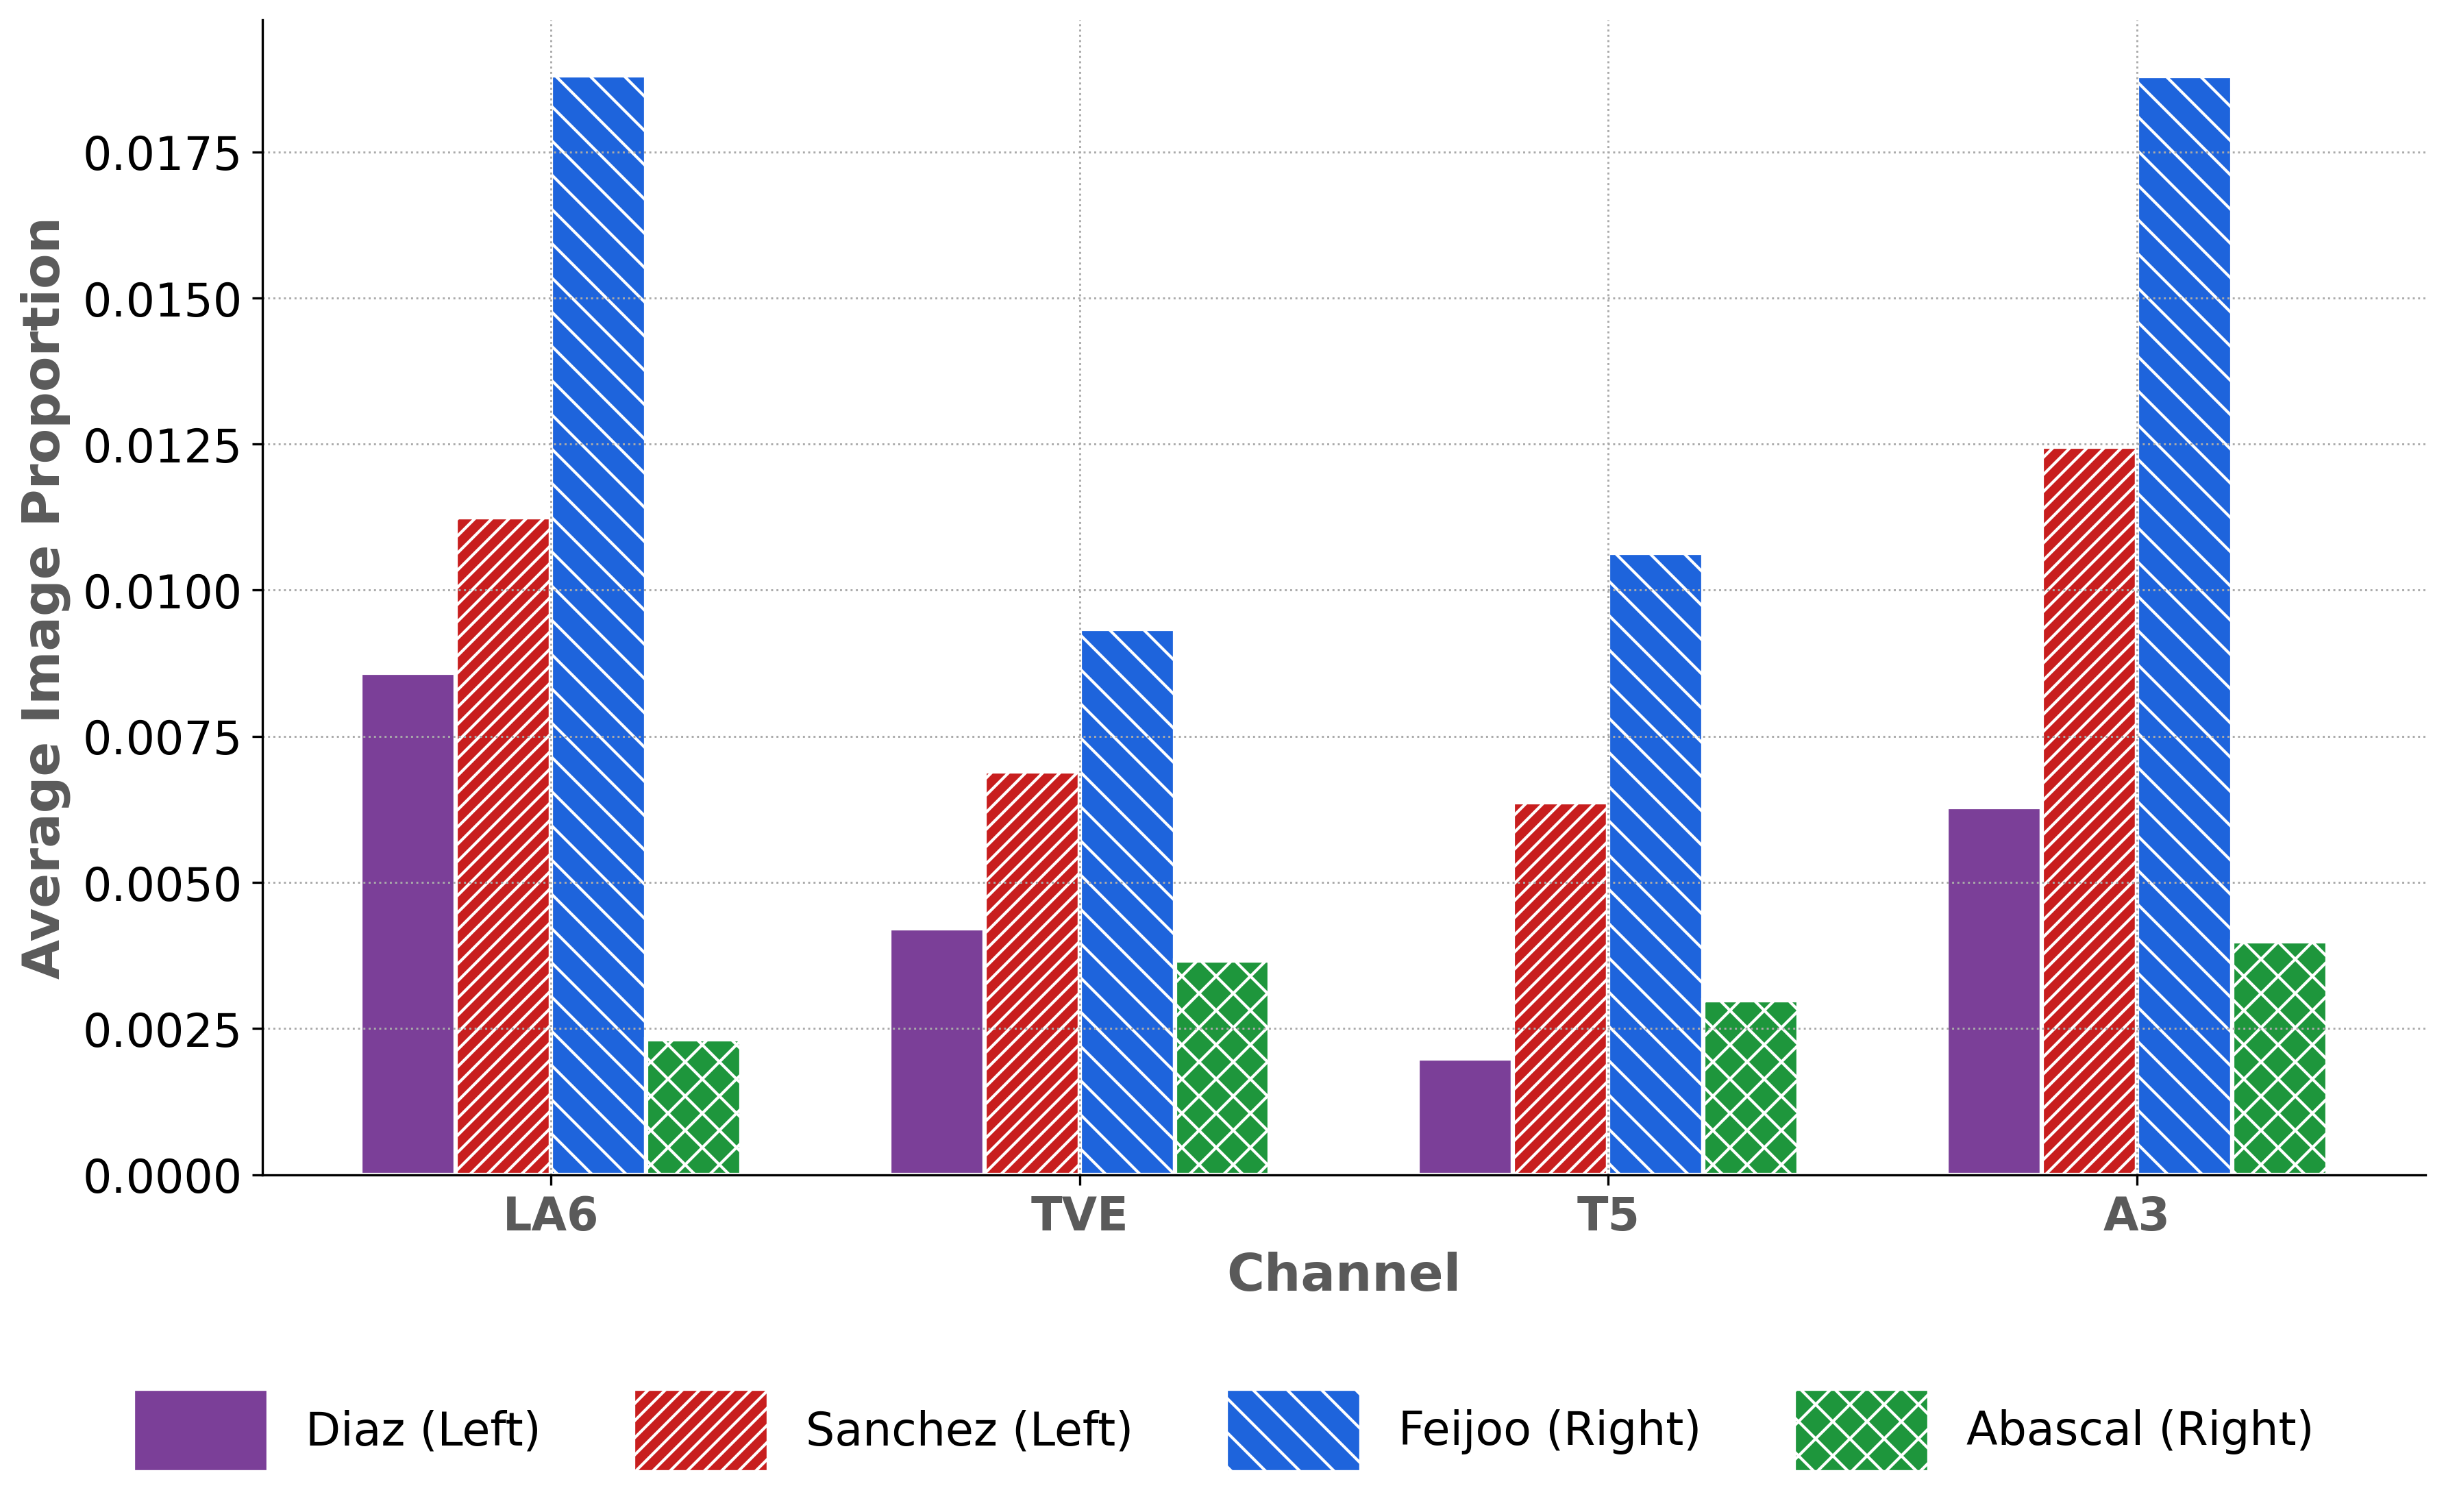
\includegraphics[width=150mm]{figures/politicians_image_proportions}
		\caption*{\small Notes: The figure shows the relative proportion of appearances by political actor and channel for a random sample of 67 days. }
		\label{fig:image_channel}
	\end{figure}
	
	
	
		\begin{figure}[!htb]
		\caption{Proportion of text mentions per channel and politician}
		\centering
		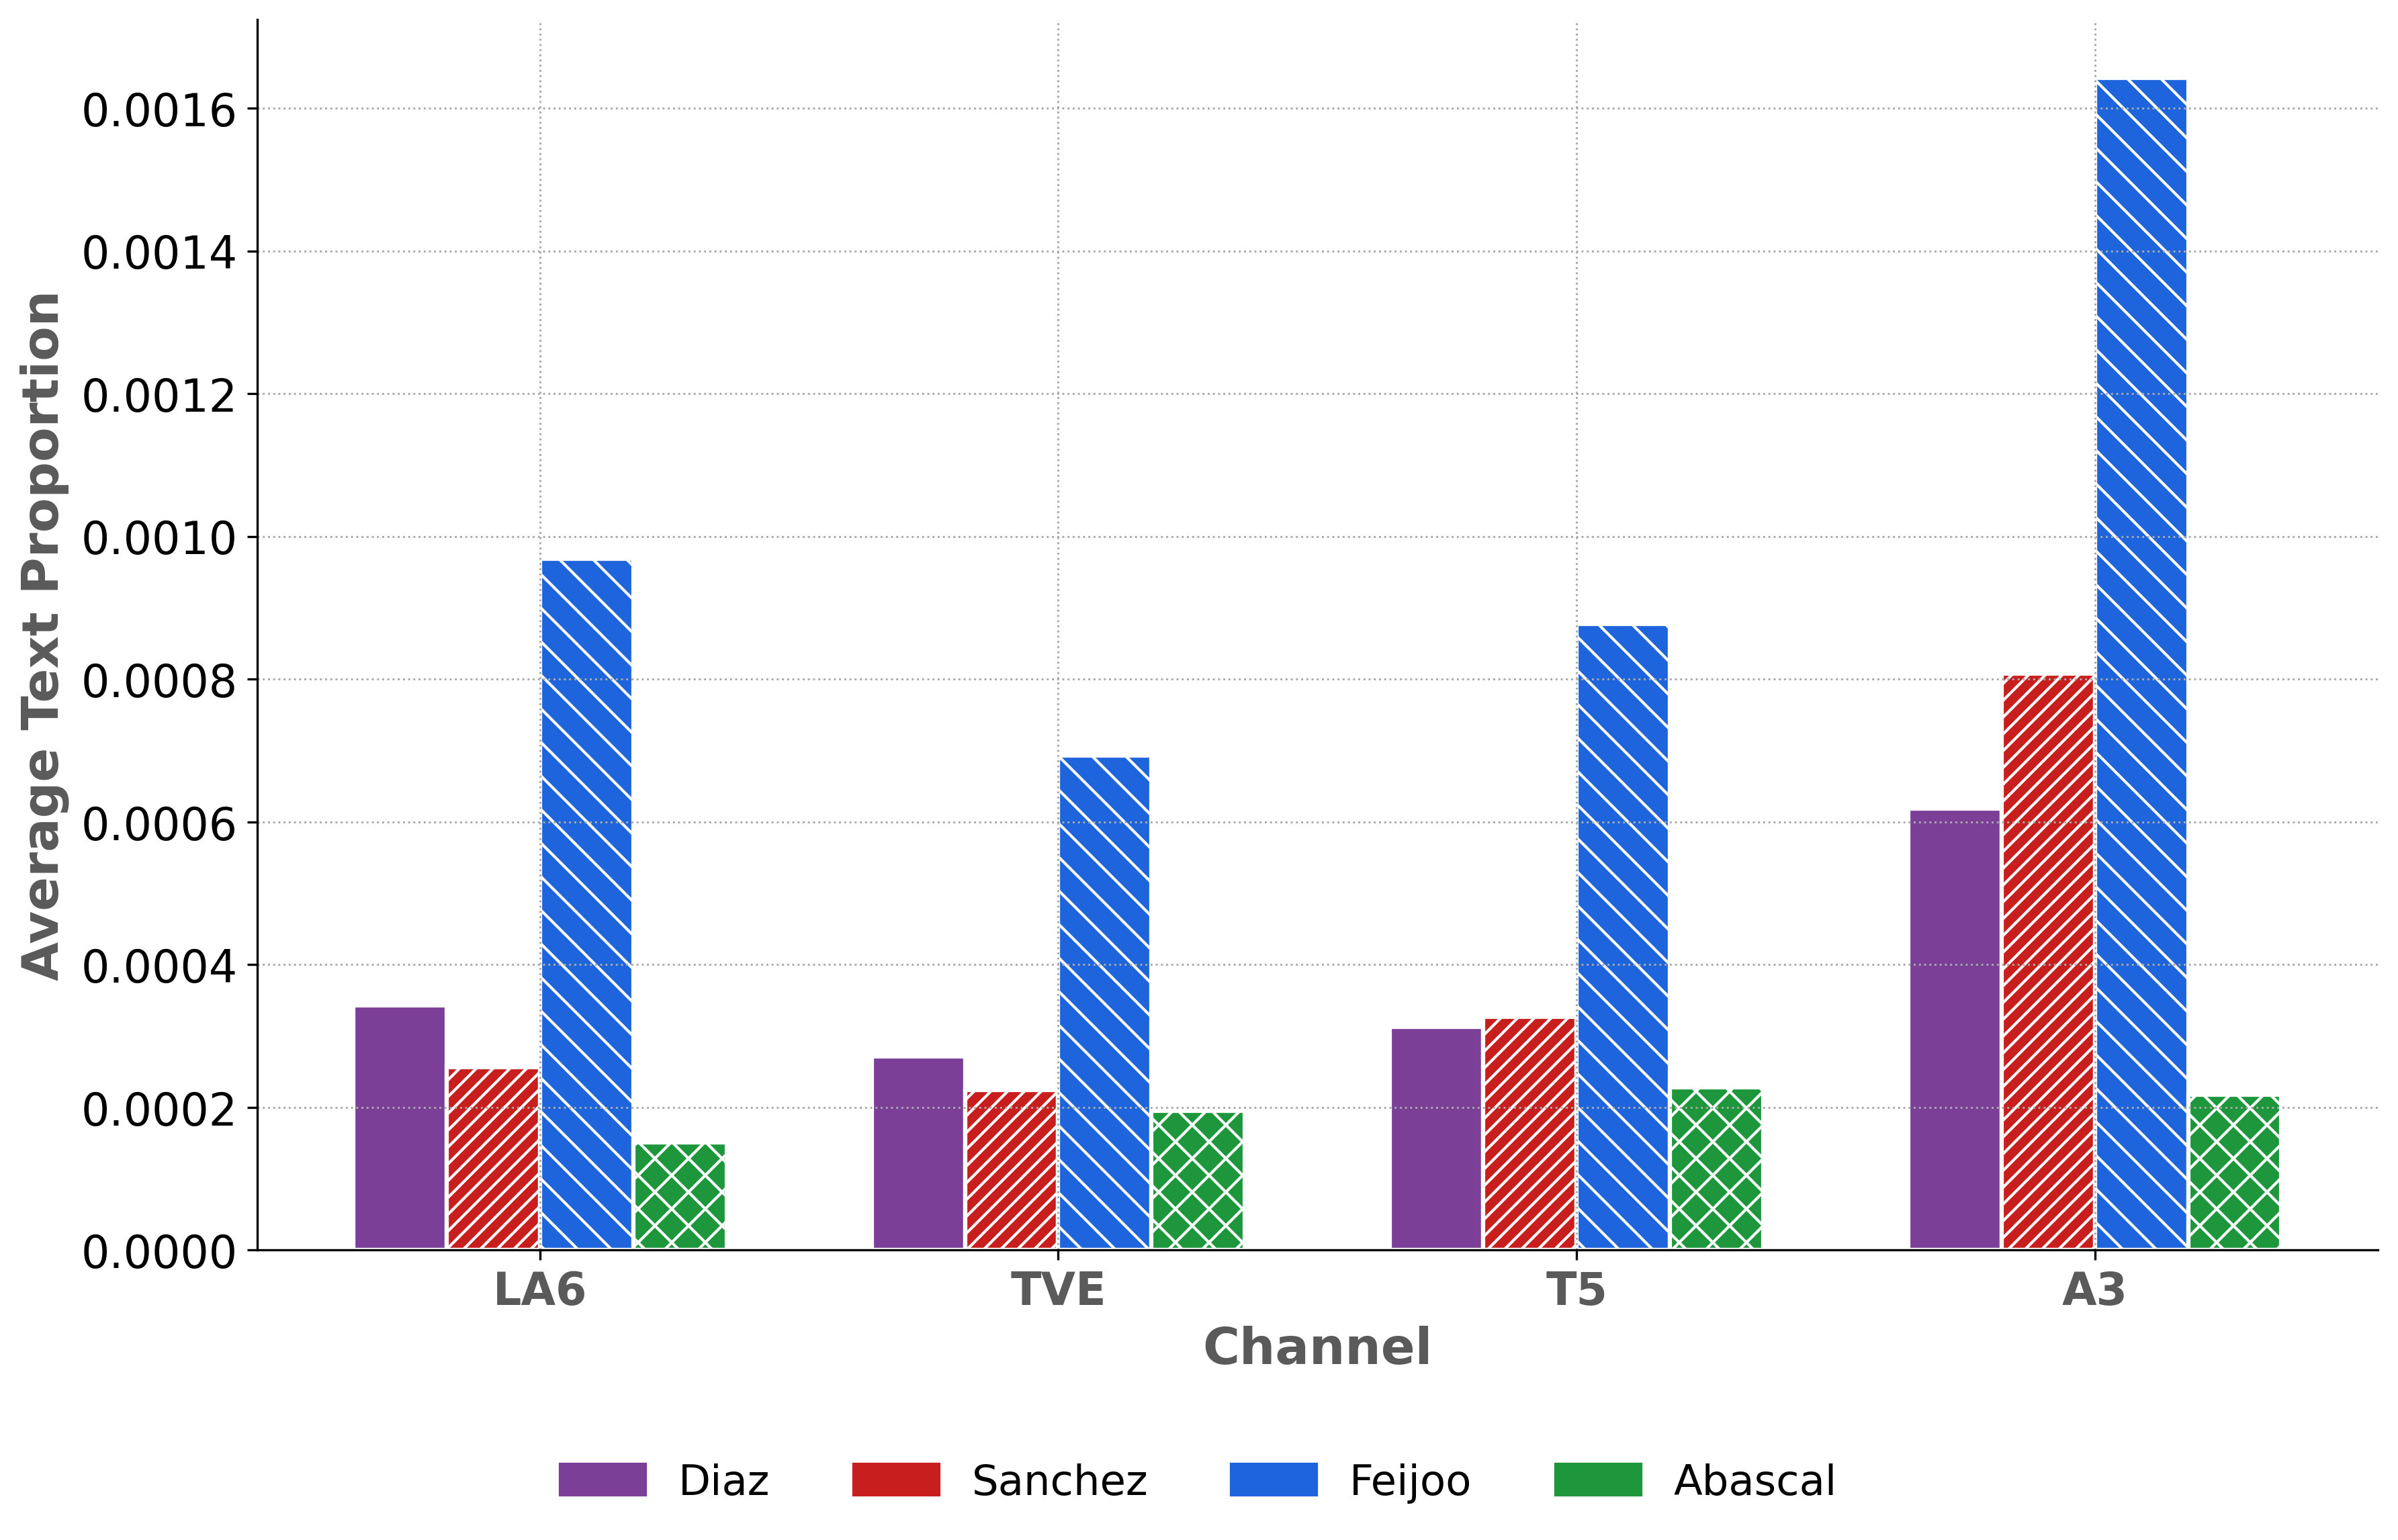
\includegraphics[width=150mm]{figures/politicians_text_proportions}
		\caption*{\small Notes: The figure shows the relative proportion of text mentions by political actor and channel for a random sample of 67 days. }
		\label{fig:mentions_channel}
	\end{figure}
	
	
		\begin{figure}[!htb]
		\caption{Net tone per channel and politician}
		\centering
		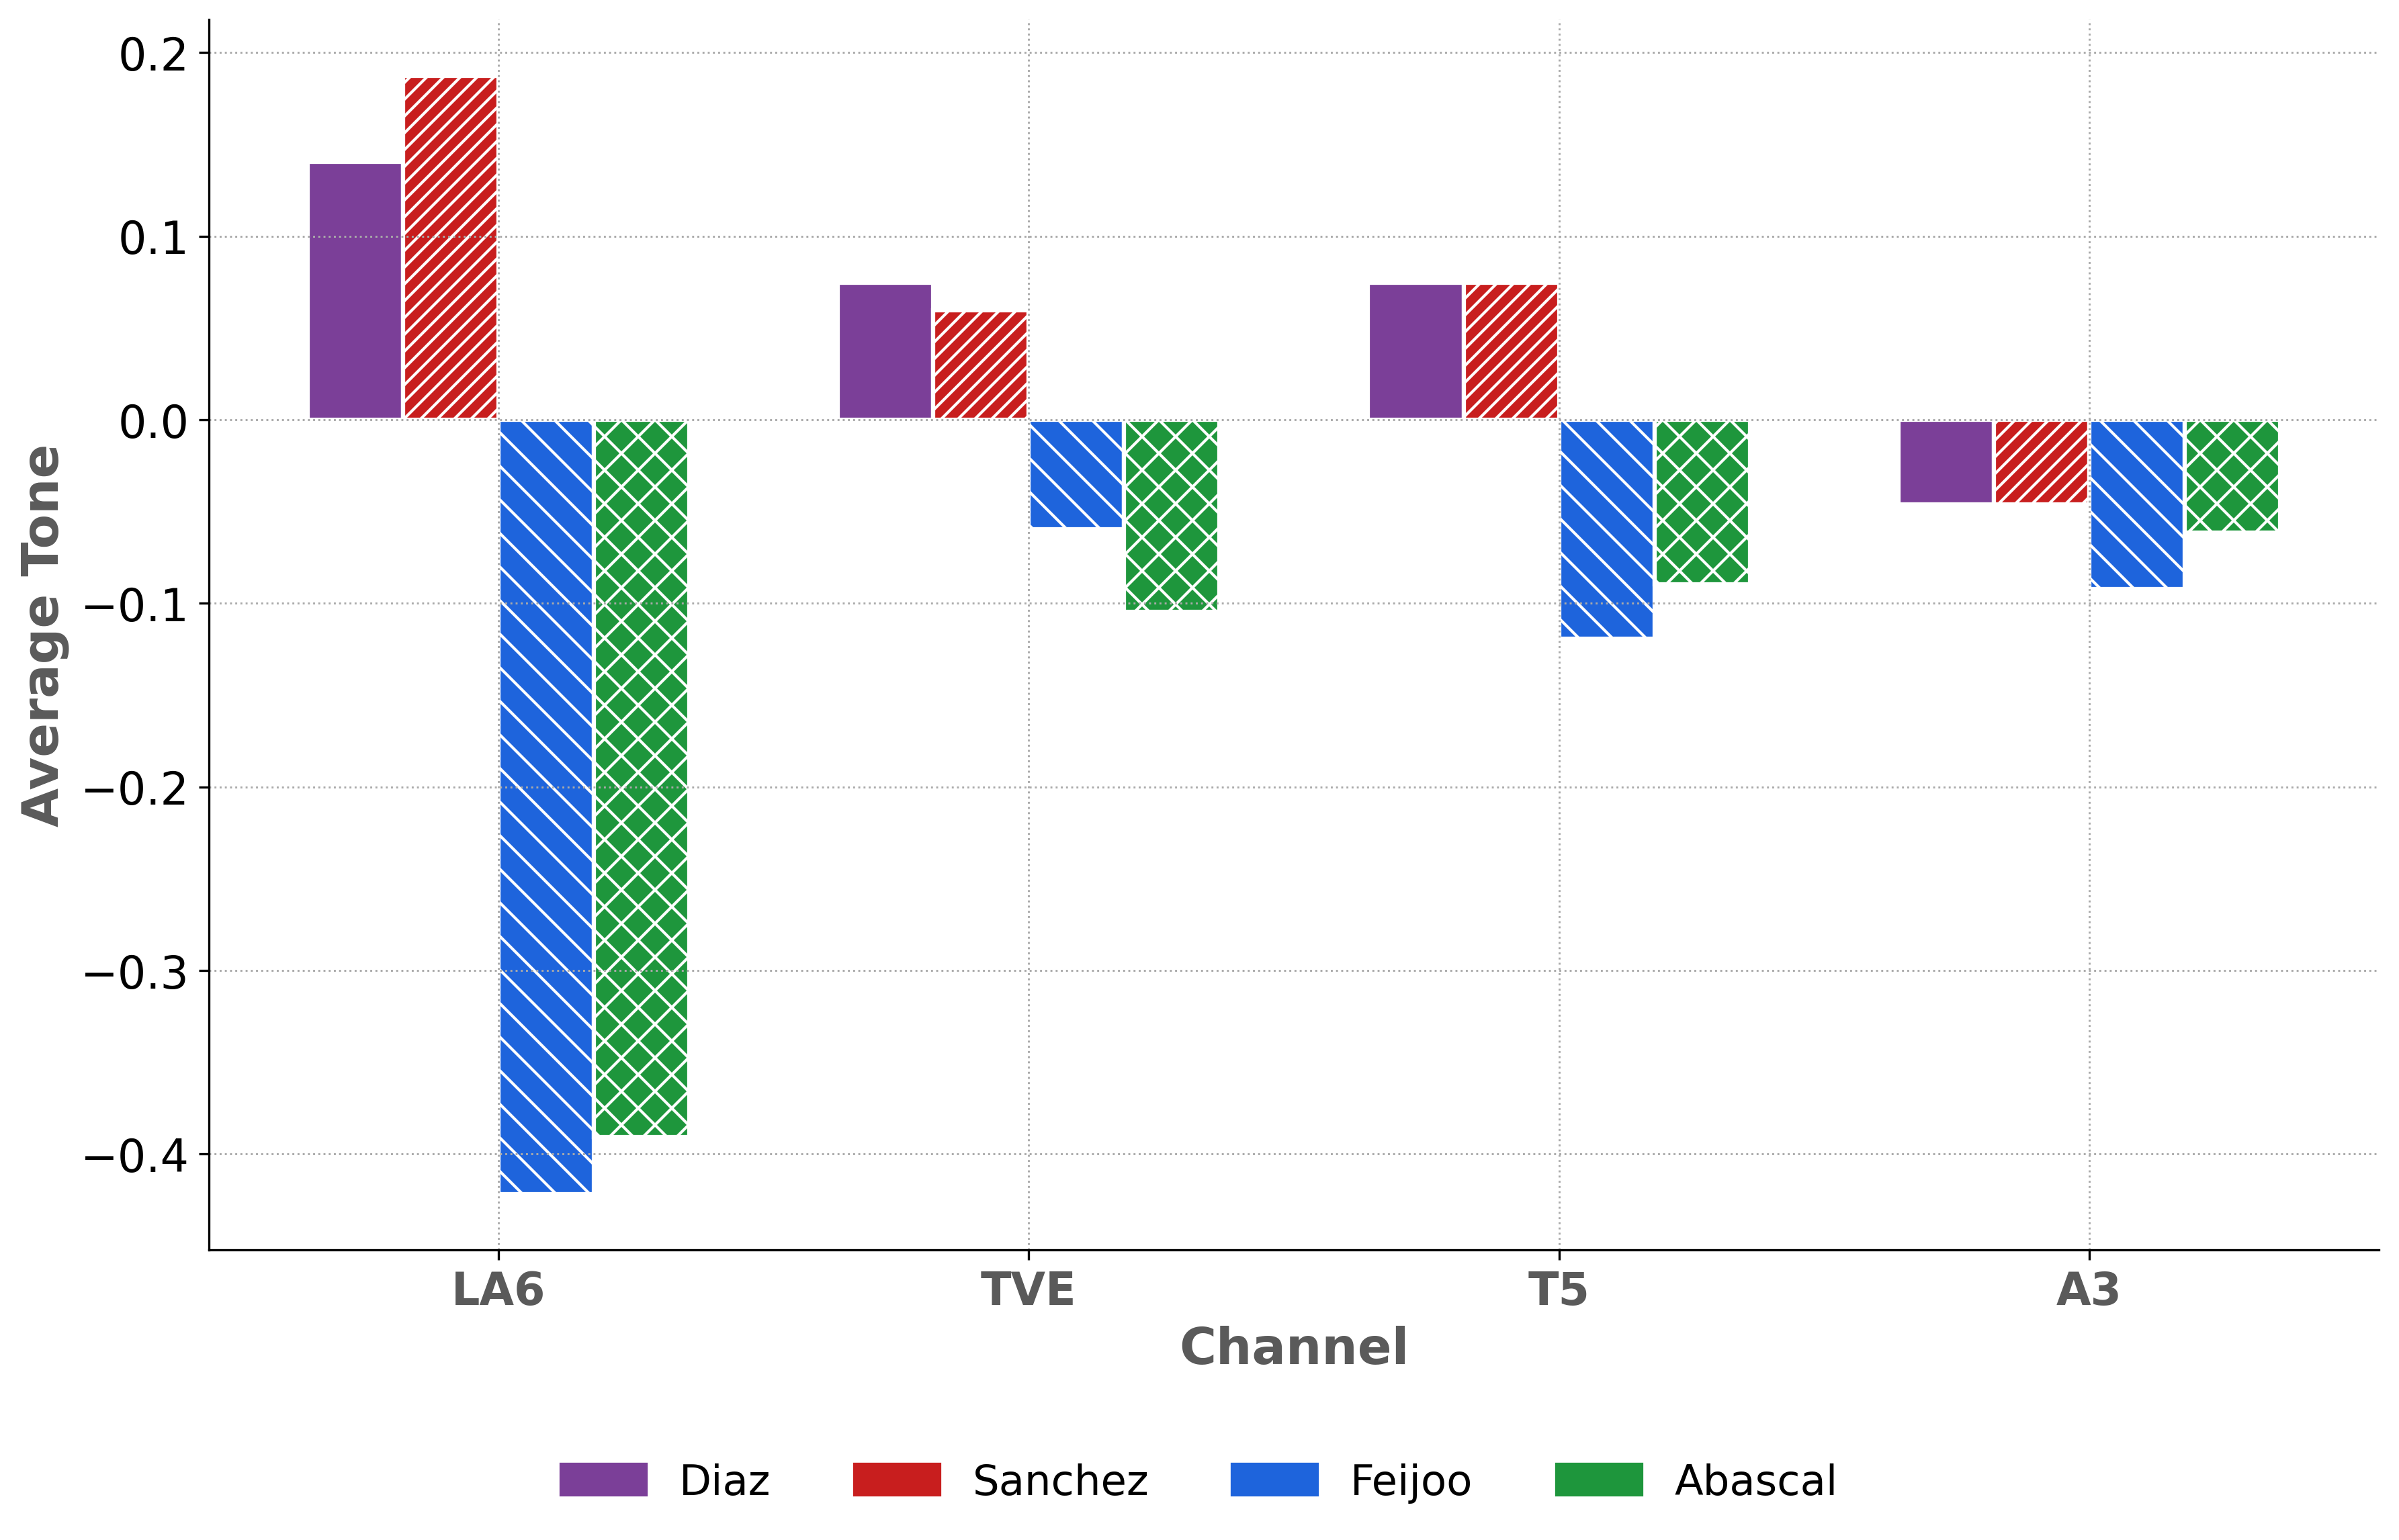
\includegraphics[width=150mm]{figures/politicians_tone_proportions}
		\caption*{\small Notes: The figure shows the net tone based on the ChatGPT classification by political actor and channel for a random sample of 67 days. }
		\label{fig:tone_channel}
	\end{figure}
	
	
	\begin{comment}
	
	\begin{figure}[H]
		\centering
		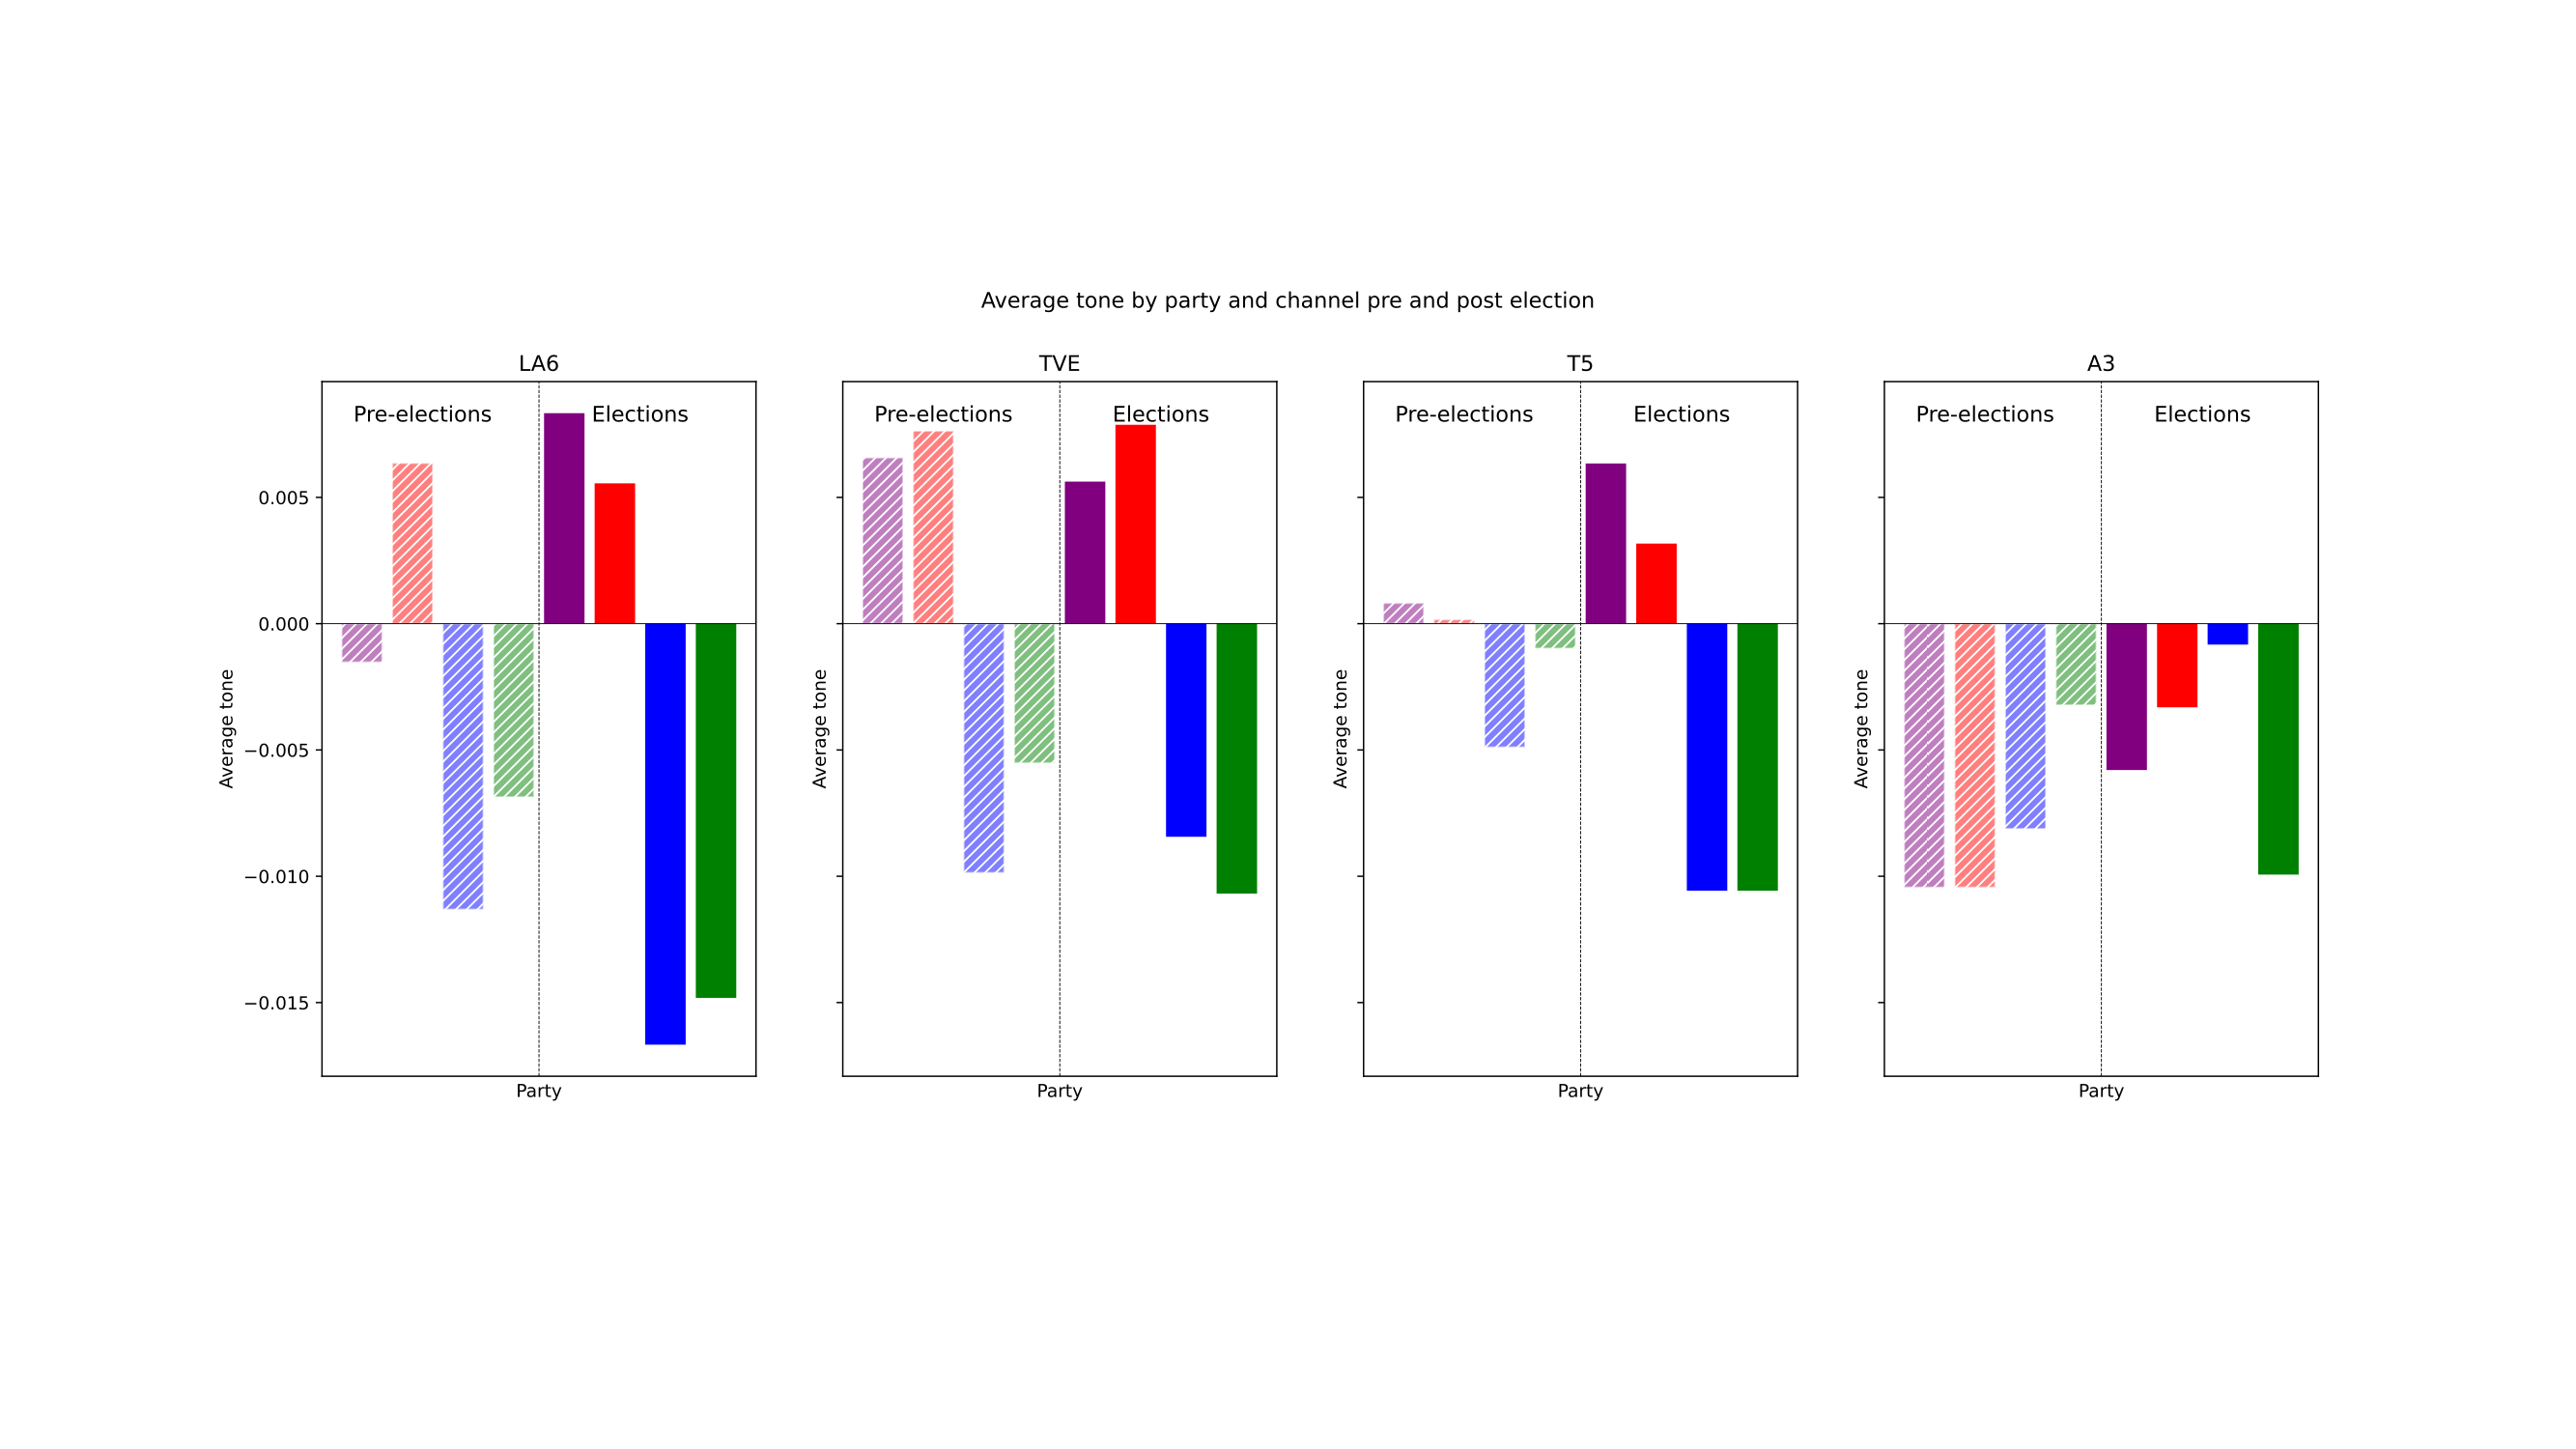
\includegraphics[width=160mm]{figures/average_tone_pre_post_election.png}
		\caption{Average tone for each party and channel pre and during campaign periods}
		\label{fig:party_decomposition}
\end{figure}
	\end{comment}	
		\begin{figure}[h!]
		\caption{Trade-offs in the model}
		\label{fig:diagram}
		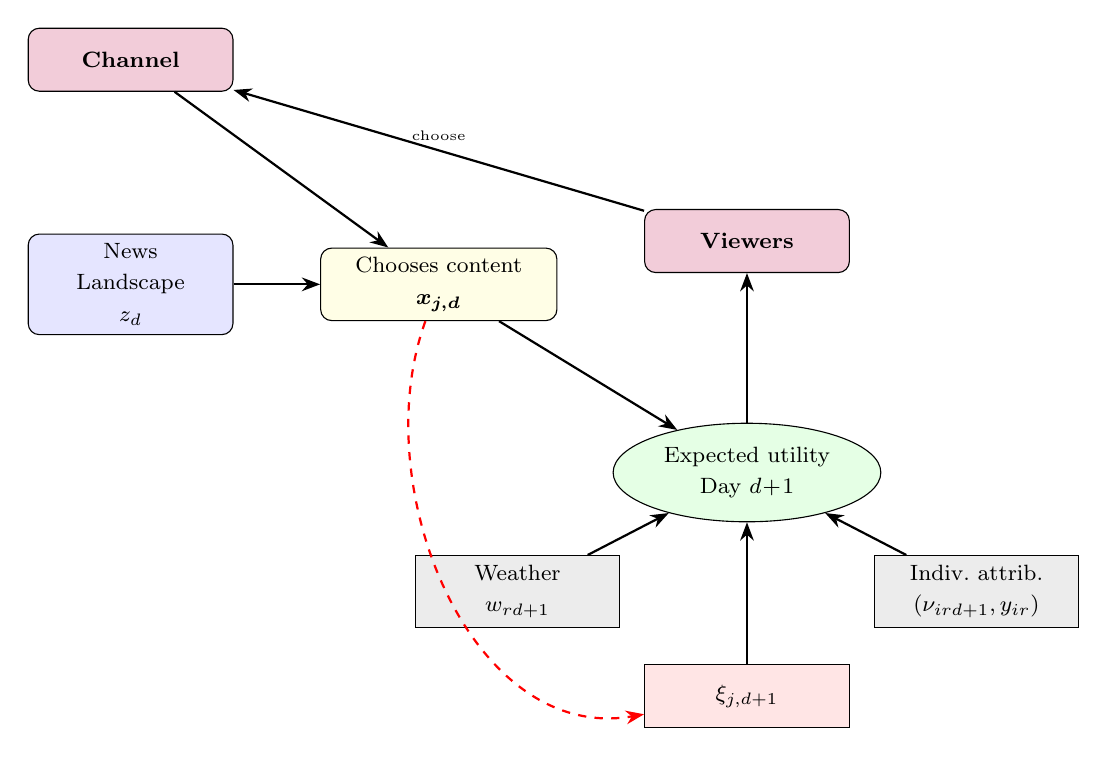
\begin{tikzpicture}[
			inst/.style   ={rectangle, draw, fill=blue!10,  rounded corners, align=center,
				minimum width=2.6cm, minimum height=0.8cm},
			decision/.style={rectangle, draw, fill=yellow!10, rounded corners, align=center,
				minimum width=3.0cm, minimum height=0.9cm},
			util/.style   ={ellipse,   draw, fill=green!10,  align=center,
				minimum width=3.4cm, minimum height=1.0cm},
			shock/.style  ={rectangle, draw, fill=red!10,   align=center,
				minimum width=2.6cm, minimum height=0.8cm},
			exo/.style    ={rectangle, draw, fill=gray!15,  align=center,
				minimum width=2.6cm, minimum height=0.8cm},
			actor/.style  ={rectangle, draw, fill=purple!20, rounded corners, align=center,
				minimum width=2.6cm, minimum height=0.8cm},
			flow/.style   ={-Stealth, thick},
			feed/.style   ={dashed,-Stealth, thick, red},
			node distance = 1.8cm and 1.1cm,
			font=\footnotesize
			]
			% -------- DAY d (supply) ---------
			\node[inst]                    (news)   {News\\Landscape\\$z_{d}$};
			\node[actor, above=of news]    (channel) {\textbf{Channel}};
			
			\node[decision, right=of news] (x)      {Chooses content\\$\bm{x_{j,d}}$};
			
			% -------- DAY d+1 (demand) ------
			\node[actor, right=of x, yshift=0.55cm] (viewer) {\textbf{Viewers}};
			
			\node[util,  below=of viewer, yshift=-0.1cm] (util)
			{Expected utility\\Day $d\!+\!1$};
			\node[shock, below=of util]     (xi)     {$\xi_{j,d+1}$};
			\node[exo,   below left=0.6cm and 0.4cm of util]
			(weather){Weather\\$w_{rd+1}$};
			\node[exo,   below right=0.6cm and 0.4cm of util]
			(prefs)  {Indiv.\ attrib.\\$(\nu_{ird+1},y_{ir})$};
			
			% ---------- flows ---------------
			\draw[flow] (channel) -- (x);
			\draw[flow] (news)    -- (x);
			\draw[flow] (x)       -- (util);
			\draw[flow] (prefs)   -- (util);
			\draw[flow] (weather) -- (util);
			\draw[flow] (xi)      -- (util);
			\draw[flow] (util)    -- (viewer) node[midway,right,font=\tiny]{};
			\draw[flow] (viewer)    -- (channel) node[midway,above,font=\tiny]{choose};
			
			
			% ------ anticipation feedback ---
			\draw[feed] (x) to[out=-110,in=190] node[midway,below,font=\tiny]
			{} (xi);
		\end{tikzpicture}
		\caption*{\small
			Notes: This diagram illustrates the structure of the model. Solid black arrows indicate causal and temporal dependencies among variables. The red dashed arrow emphasizes the simultaneity problem: content decisions $\bm{x}_{j,d}$ are made with knowledge of the future utility shock $\xi_{j,d+1}$.
		}
		
	\end{figure}
	
	
	\begin{figure}[ht!]
		\centering
		\caption{Density estimation for channels ideology based on audience share data}
		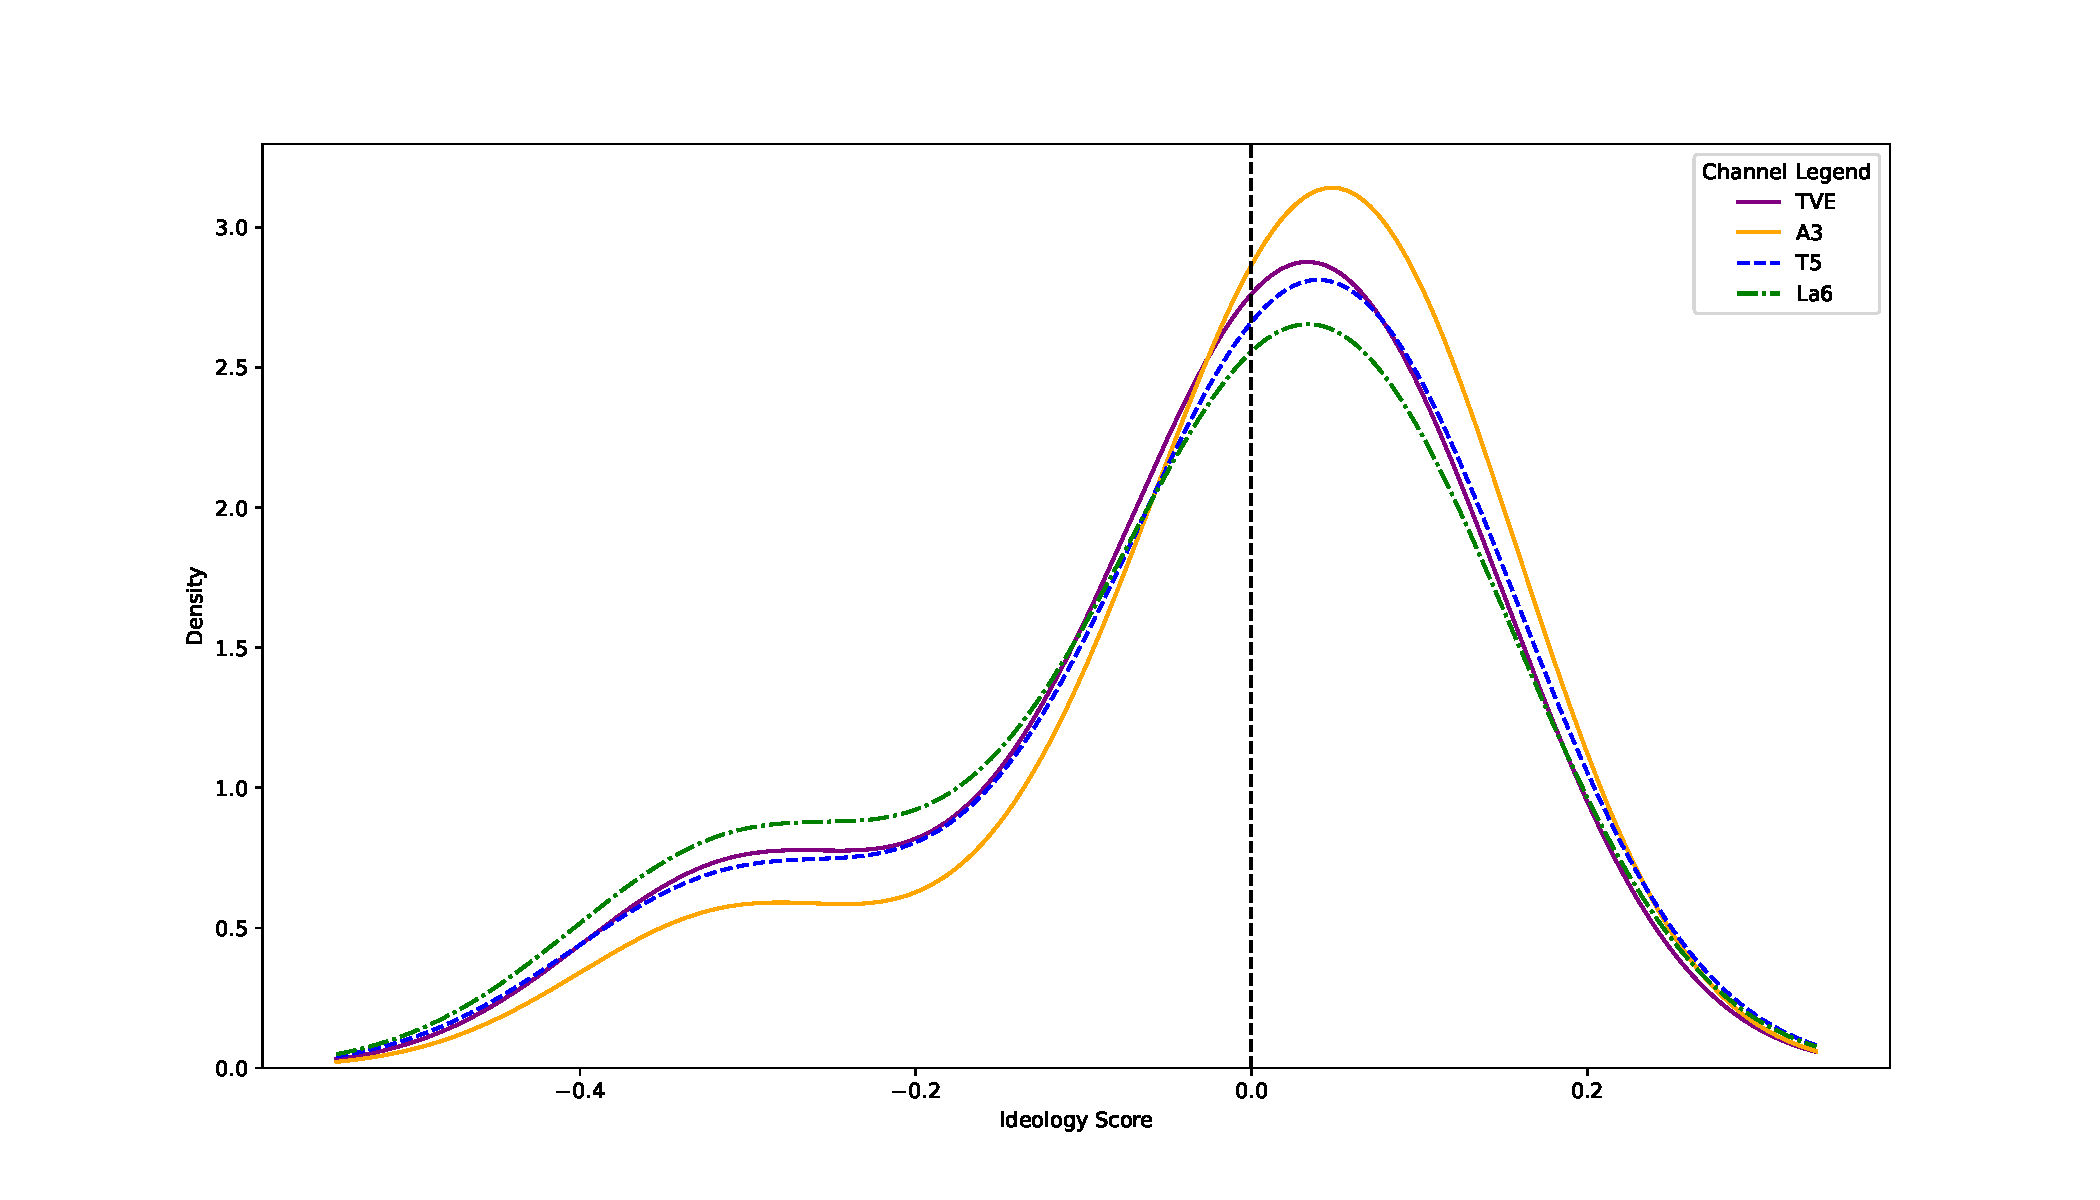
\includegraphics[width=120mm]{figures/channel_ideology_density_python}
		\caption*{\small Notes: Estimated density of channels' audience ideology. The figure shows a kernel density estimate on the ideology score constructed using survey daa and weighted by channels' share of audience for each autonomous region. }
		\label{fig:density}
	\end{figure}
	
	
		\begin{figure}[h!]
		\centering
		\caption{Added variable plots for production of political content (non-parametric fit)}
		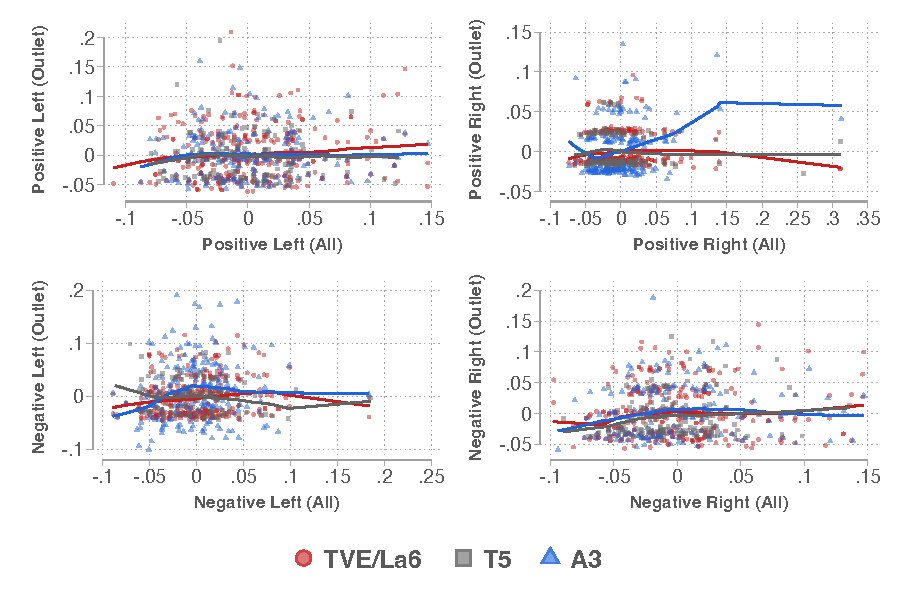
\includegraphics[width=150mm]{figures/fwl_plots_lowess}
		\caption*{\small Notes: The figure shows the added variable plots from the estimation of equation \ref{eq:first_stage}. The x axis represents $(z_d^{party,+},z_d^{party,-}) $ and the y axis the corresponding  $(x_{jd}^{party,+},x_{jd}^{party,-}) $   . Channels are pooled into left (TVE and La6), middle (T5) and right (A3) for visualization purposes.  }
		\label{fig:fwl_lowess}
	\end{figure}
	

	
	\begin{figure}[h!]
		\centering
		\caption{Added variable plots for production of political content (within day)}
		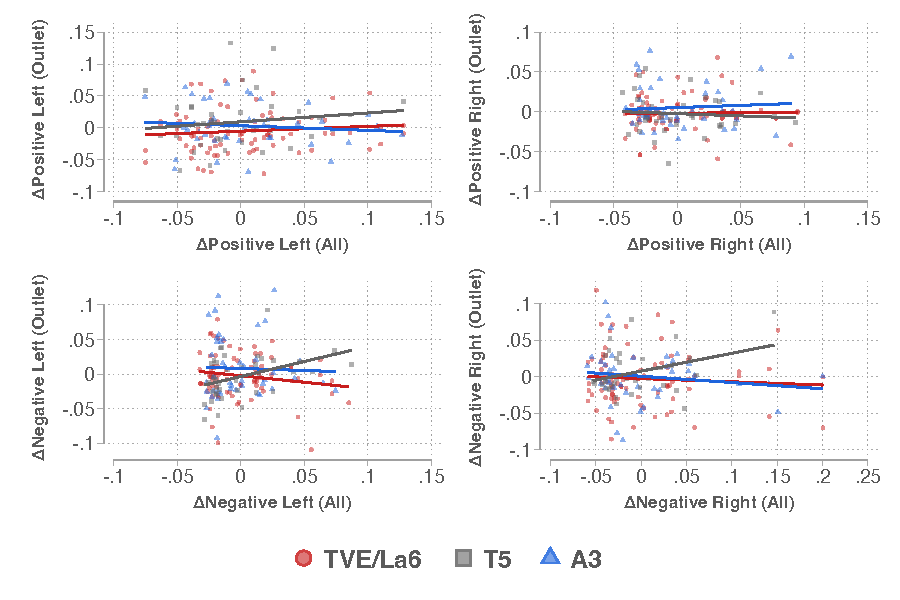
\includegraphics[width=160mm]{figures/fwl_plots_lowess_diff_costs}
		\caption*{\small Notes: The figure shows the added variable plots from the analogous estimation of equation \ref{eq:first_stage} using within day differences. The x axis represents $\left(\Delta z_d^{party,+},\Delta z_d^{party,-}\right) $ and the y axis the corresponding  $\left(\Delta x_{jd}^{party,+},\Delta x_{jd}^{party,-}\right) $   . Channels are pooled into left (TVE and La6), middle (T5) and right (A3) for visualization purposes.  }
		\label{fig:fwl_diff}
	\end{figure}
	
	
	
	\begin{figure}[ht]
		\centering
		\caption{Normalized Ideology Scores by Channel}
		% Panel (a): ChatGPT-based
		\begin{minipage}[t]{0.48\textwidth}
			\centering
			\textit{(a) Demand: Viewers' Elasticities}
			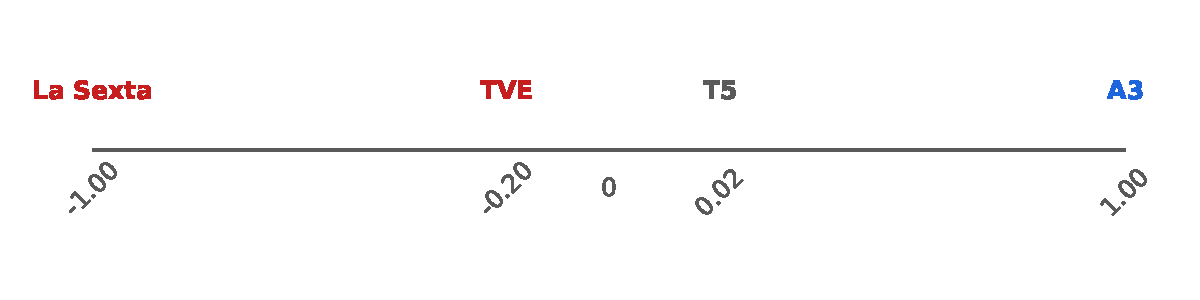
\includegraphics[width=\linewidth]{figures/congress_line_audience_share}
		\end{minipage}
		\hfill
		% Panel (b): CIS-based
		\begin{minipage}[t]{0.48\textwidth}
			\centering
			
			
			\textit{(b) Supply: ChatGPT text classification}
			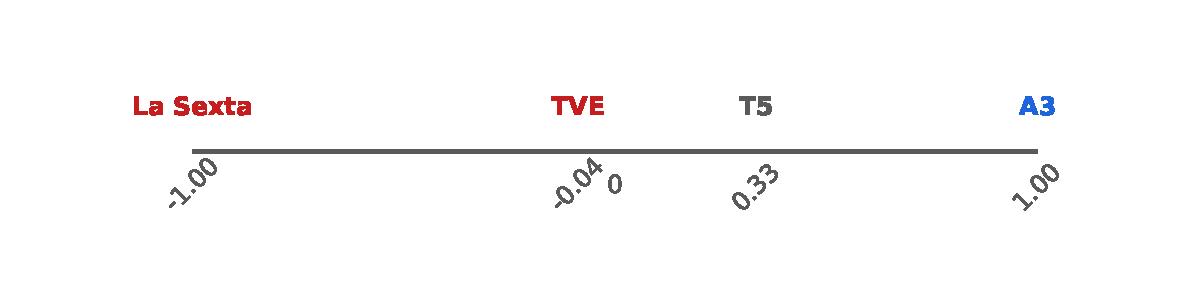
\includegraphics[width=\linewidth]{figures/congress_line_chatgpt_campaign}
			
			
		\end{minipage}
		
		
		\caption*{\small \textit{Notes:} The figure compares normalized left–right audience positions for Spanish television channels. Panel (a) positions channels according to the demand elasticities from the BLP estimation. Panel (b) shows the relative  positions of the slant for the campaign according to the ChatGPT classification. 			Channels are mapped into the $[-1,1]$ scale using their correlation (tone) and normalizing values into this scale. }
		\label{fig:channel_ideology_lines2}
	\end{figure}
	
	
	
	\begin{figure}[ht!]
		\centering
		\caption{Political and Media Polarization (no-smoothing)}
		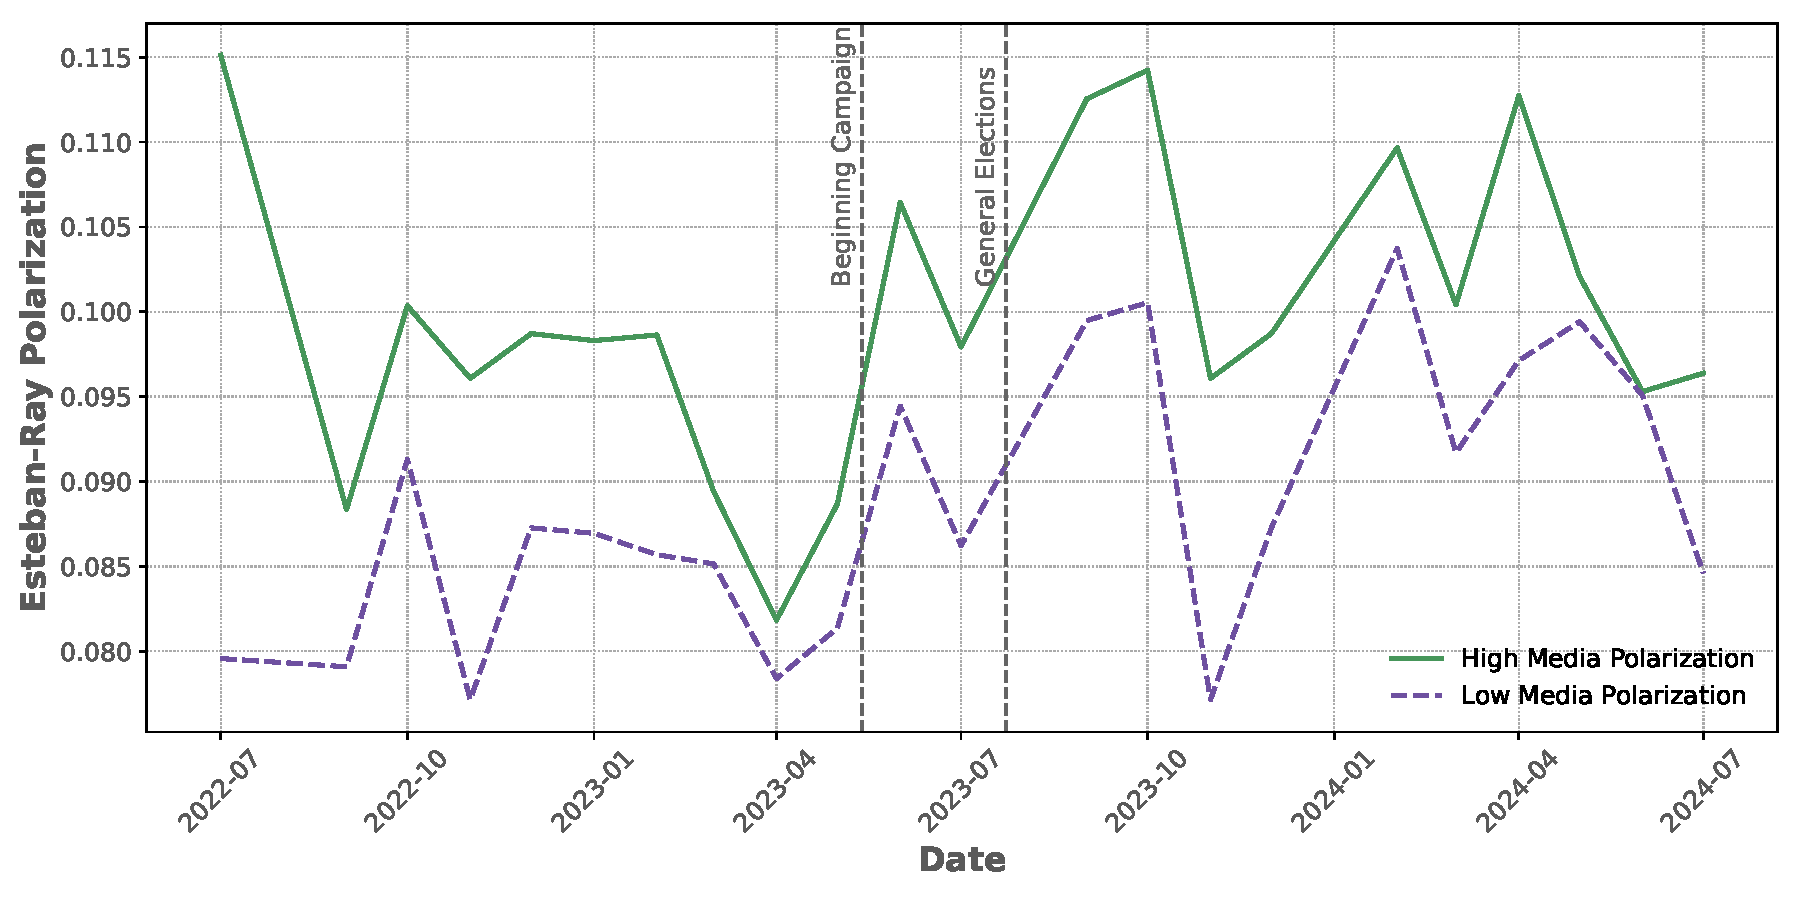
\includegraphics[width=150mm]{figures/er_polarization_stata_group_raw}
		\caption*{\textit{Note:} \small The figure shows the mean Esteban-Ray polarization index  computed as in equation \ref{eq:er}.  Solid (dashed) line represents the regions above (below) the median in terms of their media polarization consumption according to index \ref{eq:mediapol}.   }
		\label{fig:er}
	\end{figure}
	
	
	\clearpage

\section{Tables}
	
	\subsection{Additional Results}
	
	
	
	
	\begin{table}[!htb]\centering
		\def\sym#1{\ifmmode^{#1}\else\(^{#1}\)\fi}
		\caption{Effect of Mentions on Tone toward Feijóo}
		\begin{tabular}{l*{4}{c}}
			\hline\hline
			&\multicolumn{1}{c}{(1)}         &\multicolumn{1}{c}{(2)}         &\multicolumn{1}{c}{(3)}         &\multicolumn{1}{c}{(4)}         \\
			\hline
			Text Mentions   &  -25.763         &  -51.515         &   42.517         &    6.957         \\
			& (50.044)         & (51.028)         & (61.383)         & (64.934)         \\
			Image Appearances  &   -4.373         &   -2.024         &  -12.421\sym{**} &   -9.379\sym{*}  \\
			&  (3.785)         &  (3.852)         &  (4.815)         &  (5.112)         \\
			constant          &   -0.088         &   -0.093         &   -0.049         &   -0.053         \\
			&  (0.076)         &  (0.077)         &  (0.093)         &  (0.101)         \\
			Channel FE      &       No         &      Yes         &       No         &      Yes         \\
			Date FE         &       No         &       No         &      Yes         &      Yes         \\
			\hline
			Observations    &      238         &      238         &      234         &      234         \\
			\hline\hline
		\end{tabular}
		\label{tab:feijoo_images}
		\vspace{0.5em}
		\caption*{\scriptsize\emph{Note:} Robust standard errors in parentheses. The table shows the estimated coefficients for a regression of net tone on the People's Party calculated as in \ref{eq:controls}, on the proportion of image appearances and text mentions of its party leader, Feijoo. Results are for a random sample of 67 days. }
	\end{table}
	
	
	\begin{table}[!htb]\centering
		\def\sym#1{\ifmmode^{#1}\else\(^{#1}\)\fi}
		\caption{Effect of Mentions on Tone toward Abascal}
		\begin{tabular}{l*{4}{c}}
			\hline\hline
			&\multicolumn{1}{c}{(1)}         &\multicolumn{1}{c}{(2)}         &\multicolumn{1}{c}{(3)}         &\multicolumn{1}{c}{(4)}         \\
			\hline
			Text Mentions   & -506.623\sym{***}& -534.081\sym{***}& -539.867\sym{***}& -609.038\sym{***}\\
			&(148.973)         &(147.122)         &(161.979)         &(156.866)         \\
			Image Appearances  &   18.013\sym{**} &   15.994\sym{*}  &   22.023\sym{**} &   17.193\sym{*}  \\
			&  (9.077)         &  (8.996)         & (10.119)         &  (9.898)         \\
			constant          &   -0.122\sym{**} &   -0.109\sym{*}  &   -0.130\sym{**} &   -0.099\sym{*}  \\
			&  (0.057)         &  (0.056)         &  (0.057)         &  (0.056)         \\
			Channel FE      &       No         &      Yes         &       No         &      Yes         \\
			Date FE         &       No         &       No         &      Yes         &      Yes         \\
			\hline
			Observations    &      238         &      238         &      234         &      234         \\
			\hline\hline
		\end{tabular}
		\label{tab:abascal_images}
		\vspace{0.5em}
		\caption*{\scriptsize\emph{Note:} Robust standard errors in parentheses. The table shows the estimated coefficients for a regression of net tone on VOX calculated as in \ref{eq:controls}, on the proportion of image appearances and text mentions of its party leader, Abascal. Results are for a random sample of 67 days. }
	\end{table}
	
	
	\begin{table}[!htb]\centering
		\def\sym#1{\ifmmode^{#1}\else\(^{#1}\)\fi}
		\caption{Effect of Mentions on Tone toward Sánchez}
		\begin{tabular}{l*{4}{c}}
			\hline\hline
			&\multicolumn{1}{c}{(1)}         &\multicolumn{1}{c}{(2)}         &\multicolumn{1}{c}{(3)}         &\multicolumn{1}{c}{(4)}         \\
			\hline
			Text Mentions   &   61.471         &  196.424         &   27.282         &  193.827         \\
			&(106.565)         &(123.145)         &(119.969)         &(145.161)         \\
			Image Appearances  &   -2.352         &   -4.286         &   -7.639         &  -10.754         \\
			&  (4.253)         &  (4.331)         &  (6.583)         &  (6.971)         \\
			constant          &    0.054         &    0.014         &    0.120         &    0.077         \\
			&  (0.063)         &  (0.067)         &  (0.075)         &  (0.085)         \\
			Channel FE      &       No         &      Yes         &       No         &      Yes         \\
			Date FE         &       No         &       No         &      Yes         &      Yes         \\
			\hline
			Observations    &      238         &      238         &      234         &      234         \\
			\hline\hline
		\end{tabular}
		\label{tab:sanchez_images}
		\vspace{0.5em}
		\caption*{\scriptsize\emph{Note:} Robust standard errors in parentheses. The table shows the estimated coefficients for a regression of net tone on PSOE calculated as in \ref{eq:controls}, on the proportion of image appearances and text mentions of its party leader, Sánchez. Results are for a random sample of 67 days. }
	\end{table}
	
	
	\begin{table}[!htb]\centering
		\def\sym#1{\ifmmode^{#1}\else\(^{#1}\)\fi}
		\caption{Effect of Mentions on Tone toward Díaz}
		\begin{tabular}{l*{4}{c}}
			\hline\hline
			&\multicolumn{1}{c}{(1)}         &\multicolumn{1}{c}{(2)}         &\multicolumn{1}{c}{(3)}         &\multicolumn{1}{c}{(4)}         \\
			\hline
			Text Mentions   &  -11.990         &   21.235         &  -78.607         &  -19.353         \\
			& (67.519)         & (69.918)         & (91.794)         & (99.632)         \\
			Image Appearances  &    0.019         &   -0.072         &   -0.861         &   -1.032\sym{*}  \\
			&  (0.512)         &  (0.517)         &  (0.595)         &  (0.603)         \\
			constant          &    0.064         &    0.051         &    0.103\sym{**} &    0.080         \\
			&  (0.044)         &  (0.045)         &  (0.051)         &  (0.054)         \\
			Channel FE      &       No         &      Yes         &       No         &      Yes         \\
			Date FE         &       No         &       No         &      Yes         &      Yes         \\
			\hline
			Observations    &      238         &      238         &      234         &      234         \\
			\hline\hline
		\end{tabular}
		\label{tab:diaz_images}
		\vspace{0.5em}
		\caption*{\scriptsize\emph{Note:} Robust standard errors in parentheses. The table shows the estimated coefficients for a regression of net tone on UP calculated as in \ref{eq:controls}, on the proportion of image appearances and text mentions of its party leader, Díaz. Results are for a random sample of 67 days. }
	\end{table}
	

\begin{table}[htbp]
	\centering
	\scriptsize
	\setlength{\tabcolsep}{4pt}
	\renewcommand{\arraystretch}{0.9}
	\def\sym#1{\ifmmode^{#1}\else\(^{#1}\)\fi}
	\caption{First Stage Regressions}
	\label{tab:first_stage}
	\begin{tabular}{lcccc}
		\hline\hline
		& \multicolumn{1}{c}{(1) Positive Right}
		& \multicolumn{1}{c}{(2) Negative Right}
		& \multicolumn{1}{c}{(3) Positive Left}
		& \multicolumn{1}{c}{(4) Negative Left} \\
		\hline
		\multicolumn{5}{l}{\textbf{Positive Right (All)}}\\
				\hline
		TVE            &  0.00342         & -0.00456         & -0.0498         & -0.0916         \\
		&  (0.08)          & (-0.07)          & (-0.71)         & (-1.30)         \\
		A3             &  0.207\sym{***}  & -0.139           & -0.0615         & -0.113          \\
		&  (4.62)          & (-1.89)          & (-0.81)         & (-1.47)         \\
		T5             & -0.0372          & -0.0746          & -0.0943         & -0.166\sym{*}   \\
		& (-0.88)          & (-1.08)          & (-1.31)         & (-2.28)         \\
		La Sexta       &  0.0334          & -0.0129          &  0.0290         & -0.0256         \\
		&  (0.73)          & (-0.17)          &  (0.37)         & (-0.33)         \\
		\hline
		\multicolumn{5}{l}{\textbf{Negative Right (All)}}\\
				\hline
		TVE            & -0.0296          &  0.00590         & -0.0707         &  0.0738         \\
		& (-0.74)          &  (0.09)          & (-1.04)         &  (1.08)         \\
		A3             & -0.0333          &  0.0929          & -0.0104         & -0.0440         \\
		& (-0.79)          &  (1.34)          & (-0.14)         & (-0.61)         \\
		T5             & -0.0585          &  0.131           &  0.0327         & -0.0166         \\
		& (-1.05)          &  (1.44)          &  (0.35)         & (-0.17)         \\
		La Sexta       & -0.0185          &  0.143\sym{*}    & -0.0399         & -0.123          \\
		& (-0.42)          &  (1.97)          & (-0.53)         & (-1.63)         \\
		\hline
		\multicolumn{5}{l}{\textbf{Positive Left (All)}}\\
				\hline
		TVE            &  0.0261         &  0.0634         &  0.200\sym{**}  & -0.0511         \\
		&  (0.68)         &  (1.01)         &  (3.07)         & (-0.78)         \\
		A3             &  0.00911        & -0.0626         &  0.0154         & -0.0845         \\
		&  (0.22)         & (-0.92)         &  (0.22)         & (-1.19)         \\
		T5             & -0.0712         & -0.159          & -0.00405        & -0.0572         \\
		& (-1.43)         & (-1.95)         & (-0.05)         & (-0.67)         \\
		La Sexta       &  0.00655        & -0.0906         & -0.00875        &  0.0718         \\
		&  (0.16)         & (-1.33)         & (-0.12)         &  (1.01)         \\
		\hline
		\multicolumn{5}{l}{\textbf{Negative Left (All)}}\\
				\hline
		TVE            &  0.0144         & -0.0603         & -0.176\sym{*}   &  0.149          \\
		&  (0.32)         & (-0.81)         & (-2.26)         &  (1.90)         \\
		A3             &  0.0446         & -0.133          & -0.173\sym{*}   &  0.184\sym{*}   \\
		&  (0.93)         & (-1.69)         & (-2.11)         &  (2.23)         \\
		T5             & -0.141\sym{**}  &  0.0136         & -0.00461        & -0.0569         \\
		& (-2.66)         &  (0.16)         & (-0.05)         & (-0.63)         \\
		La Sexta       &  0.0262         & -0.141          & -0.139          &  0.111          \\
		&  (0.53)         & (-1.73)         & (-1.65)         &  (1.31)         \\
		\hline
		\multicolumn{5}{l}{\textbf{Political (All)}}\\
				\hline
		TVE            &  0.0167         &  0.0680\sym{*}  &  0.0828\sym{*}  &  0.0494         \\
		&  (0.82)         &  (2.03)         &  (2.38)         &  (1.41)         \\
		A3             &  0.0187         &  0.145\sym{***}&  0.137\sym{***}&  0.175\sym{***}\\
		&  (0.84)         &  (3.98)         &  (3.62)         &  (4.59)         \\
		T5             &  0.0975\sym{***}&  0.0981\sym{*}  &  0.0837         &  0.125\sym{**}  \\
		&  (3.69)         &  (2.26)         &  (1.86)         &  (2.77)         \\
		La Sexta       &  0.0145         &  0.132\sym{***}&  0.123\sym{**} &  0.0393         \\
		&  (0.63)         &  (3.47)         &  (3.12)         &  (0.99)         \\
		\hline\hline
	\end{tabular}
	
	\caption*{\scriptsize\emph{Note:} Robust standard errors in  parentheses;\quad \sym{*} $p<0.05$, \sym{**} $p<0.01$, \sym{***} $p<0.001$. The table shows the results of the first stage regressions in equation \ref{eq:first_stage}. The total number of observations is $N=687$ }
	

\end{table}

	
	
	
	
	
	
	\begin{table}[!htb]
		\label{tab:logit}
		\centering
		\begin{threeparttable}
			\begin{tabular}{lccc}
				\hline
				\textbf{Coefficient} & \textbf{Parameter} & \textbf{Estimate} & \textbf{Std.\ Error} \\
				\hline
				\hline
				\multicolumn{4}{c}{\textbf{Pre-campaign}} \\
				\hline
				Positive Left & $\beta^{L+}$ & -17.62 & (14.344) \\
				Positive Right & $\beta^{R+}$ & -41.16** & (18.718) \\
				Negative Left & $\beta^{L-}$ & 27.24 & (20.268) \\
				Negative Right & $\beta^{R-}$ & 66.04* & (34.668) \\
				Political & $\beta^{political}$ & 14.28* & (7.465) \\
				Weather & $\gamma$ & 0.01 & (0.655) \\
				Positive Left $\times$ Right-Mean & $\phi^{L+}$ & 47.67 & (36.262) \\
				Positive Right $\times$ Right-Mean & $\phi^{R+}$ & 111.13** & (50.798) \\
				Negative Left $\times$ Right-Mean & $\phi^{L-}$ & -81.40 & (51.195) \\
				Negative Right $\times$ Right-Mean & $\phi^{R-}$ & -151.24* & (89.249) \\
				Political $\times$ Right-Mean & $\phi^{political}$ & -30.80 & (18.952) \\
				\hline
				\hline
				\multicolumn{4}{c}{\textbf{Campaign}} \\
				\hline
				Positive Left & $\beta^{L+}$ & 222.18** & (110.419) \\
				Positive Right & $\beta^{R+}$ & -177.76** & (88.006) \\
				Negative Left & $\beta^{L-}$ & -153.39** & (76.074) \\
				Negative Right & $\beta^{R-}$ & 147.85** & (69.428) \\
				Political & $\beta^{political}$ & -10.37** & (5.107) \\
				Weather & $\gamma$ & 0.80*** & (0.287) \\
				Positive Left $\times$ Right-Mean & $\phi^{L+}$ & -619.77** & (303.679) \\
				Positive Right $\times$ Right-Mean & $\phi^{R+}$ & 461.19* & (242.882) \\
				Negative Left $\times$ Right-Mean & $\phi^{L-}$ & 398.26* & (211.132) \\
				Negative Right $\times$ Right-Mean & $\phi^{R-}$ & -413.87** & (187.584) \\
				Political $\times$ Right-Mean & $\phi^{political}$ & 28.91** & (14.181) \\
				\hline
			\end{tabular}
			\caption{Logit Estimation Results with Standard Errors}
				\begin{tablenotes}
				\small
				\item \footnotesize{The table shows the results of the logit estimation of model \ref{eq:logit}. The estimations are divided into the pre-campaign and campaign period. Both day-of-the-week and outlet fixed effects are included. Standard errors are clustered at the region level. The total number of observations are $N_{campaign}=2307$ and  $N_{pre\_campaign}=6604$.}
			\end{tablenotes}
		\end{threeparttable}
	\end{table}
	
	
	
\begin{table}[!htb]
	\centering
	\caption{Top 5 Topics by party-tone category on Agencia EFE after BERTopic. }
	\begin{tabular}{|l|c|}
		\hline
				\multicolumn{1}{|c|}{\textbf{Topic Words}}& \textbf{Count} \\
		\hline
		\hline
		\multicolumn{2}{|c|}{\textbf{Positive Right}} \\
		\hline
		vox, motion, abascal, censure, pp, tamames, santiago, garriga, parties, party & 312 \\
		feijóo, núñez, alberto, pp, leader, gamarra, parties, party, general, cuca & 113 \\
		guardiola, extremadura, mérida, maría, vara, extremeño, council, assembly, candidate & 68 \\
		mazón, valencian, president, corts, valencian, valencians, government, carlos & 64 \\
		electoral, elections, general, jec, board, campaign, 28m, 23j, vote & 63 \\
		\hline
		\multicolumn{2}{|c|}{\textbf{Negative Right}} \\
		\hline
		vox, motion, abascal, censure, pp, tamames, santiago, garriga, parties, party & 369 \\
		abortion, castilla, healthcare, anti-abortion,pregnancy, abortions, law, mañueco & 112 \\
		code, criminal, sedition, embezzlement, reform, crime, penalties, amendments & 81 \\
		electoral, elections, general, jec, board, campaign, 28m, 23j, vote & 71 \\
		sánchez, pedro, feijóo, president, government, núñez, leader, alberto, pp, executive & 69 \\
		\hline
		\multicolumn{2}{|c|}{\textbf{Positive Left}} \\
		\hline
		yes, only, reform, sexual, law, is, violence, reform, just, podemos & 200 \\
		sánchez, pedro, feijóo, president, government, núñez, leader, alberto, pp, executive & 183 \\
		yolanda, díaz, vice president, sumar, second, podemos, labor, leader, minister & 179 \\
		sumar, podemos, errejón, iu, íñigo, yolanda, parties, coalition, díaz, left-wing & 142 \\
		psoe, socialists, federal, secretary, parties, socialist, lobato, espadas, congress & 129 \\
		\hline
		\multicolumn{2}{|c|}{\textbf{Negative Left}} \\
		\hline
		yes, only, reform, sexual, law, is, violence, reform, just, podemos & 182 \\
		sánchez, pedro, feijóo, president, government, núñez, leader, alberto, pp, executive & 153 \\
		vox, motion, abascal, censure, pp, tamames, santiago, garriga, parties, party & 129 \\
		sexual, assault, sexually, sexual, minor, violence, assault, convicted, abuse & 108 \\
		psoe, socialists, federal, secretary, parties, socialist, lobato, espadas, congress & 72 \\
		\hline
	\end{tabular}
	\caption{Table shows the top 5 topics associated with the top stories that provided more positive/negative coverage for each party in the Agencia EFE corpus. words were translated to English with the help of ChatGPT. }
\end{table}

	
	
	
	\begin{table}[!htb]
		\centering
		\caption{Mean and Standard Error for 100 Rounds of ChatGPT Classification}
		\begin{tabular}{|l|c|c|c|c|}
			\hline
			\textbf{Statistic} & \textbf{PP} & \textbf{PSOE} & \textbf{VOX} & \textbf{UP} \\
			\hline
			Mean & -0.014 & 0.106 & -0.053 & 0.024 \\
			Standard Error & 0.003 & 0.004 & 0.001 & 0.002 \\
			\hline
		\end{tabular}
		\caption*{Note: The table shows the mean and standard error for 100 rounds of ChatGPT classification of political content with 40 random political stories.}
		\label{tab:table_stability}
	\end{table}
	
	
	
	
	
	
	\begin{table}[!htb]
		
		\caption{Estimated Elasticities by Left and Right markets}
		\begin{tabular}{l|cc|cc}
			\toprule
			& \multicolumn{2}{c|}{\textbf{Pre-campaign}} & \multicolumn{2}{c}{\textbf{Campaign}} \\
			Characteristic & Left Market & Right Market & Left Market & Right Market \\
			\midrule
			Negative Left & 1.481 & 0.136 & -0.681 & 0.380 \\
			Positive Left & -0.011 & 0.129 & 0.754 & -0.716 \\
			Negative Right & 1.358 & 0.469 & 0.462 & -0.182 \\
			Positive Right & -0.029 & 0.152 & -1.371 & 0.133 \\
			\bottomrule
		\end{tabular}
		\caption*{\textit{Note:} \small The table shows the average elasticities for each characteristic by right and left markets as defined in equation \ref{eq:elasticities}. Right markets are defined as regions with proportion of right wing voters above the median. }
		\label{tab:elasticities}
	\end{table}
	
	
	
\clearpage
	\subsection{Text Examples}
	
		\begin{table}[!htb]
		\centering
		\begin{tabular}{p{0.8\textwidth}}
			\toprule
			\textbf{Top stories for  Negative Left}  \\
			\midrule
			-Reduction of a convicted rapist’s sentence in Salamanca under the "Solo sí es sí" law  \\
			-Seville Court reduces a murder and sexual assault sentence by 5 years due to the "Solo sí es sí" law  \\
			-Vox formally submits a motion of no confidence against Prime Minister Pedro Sánchez  \\
			-Madrid’s regional president, Isabel Díaz Ayuso, predicts that the "Mediator Case" will bring down the government  \\
			\bottomrule
		\end{tabular}
		\begin{tabular}{l c}
			\toprule
			\textbf{Channel} & \textbf{Proportion of Negative Left} \\
			\midrule
			TVE & 0.037 \\
			Antena 3  & 0.184 \\
			Telecinco  & 0.037 \\
			La Sexta  & 0.01 \\
			\bottomrule
		\end{tabular}
		\caption{Top table shows the main stories contributing to negative left content on 2023-02-27, the highest day with negative left content,  summarized and translated to English by ChatGPT. Bottom table shows the proportion of minutes devoted to negative left content per channel on the same date.}
		\label{tab:neg_left_channels}
	\end{table}
	
	
		\begin{table}[!htb]
		\centering
		\begin{tabular}{p{0.8\textwidth}}
			\toprule
			\textbf{Top stories for  Negative Right}  \\
			\midrule
			-Congress declarations against Ayuso over alleged "bribes" to her brother  \\
			-Marinaleda criticizes the "abusive" arrest of two residents during a protest against Vox  \\
			-The Senate rejects a PP motion on the government's alleged partisan use of the Falcon jet  \\
			\bottomrule
		\end{tabular}
	
		

		\begin{tabular}{l c}
			\toprule
			\textbf{Channel} & \textbf{Proportion of Negative Right} \\
			\midrule
			TVE & 0.074 \\
			Antena 3  & 0.038 \\
			Telecinco  & 0.067 \\
			La Sexta  & 0.148 \\
			\bottomrule
		\end{tabular}
		\caption{Top table shows the main stories contributing to negative right content on 2023-05-17, the highest day with negative right content,  summarized and translated to English by ChatGPT. Bottom table shows the proportion of minutes devoted to negative right content per channel on the same date. }
		\label{tab:neg_right_channels}
	\end{table}
	
	\begin{table}[!htb]
		\centering
		\begin{tabular}{|l|l|}
			\hline
			Positive Right & Negative Right \\
			\hline
			vox secretary general & gürtel national service \\
			vox ignacio garriga & gürtel trial service \\
			general vox ignacio & valencia francisco camps \\
			núñez feijóo called & gürtel trial gürtel \\
			pp candidate elections & former president valencian government \\
			vox parties madrid & valencian government francisco \\
			josé sáenz buruaga & psoe deputy secretary general \\
			núñez feijóo requested & gürtel trial madrid \\
			maría josé sáenz & abortion law reform \\
			may pp president & former valencian president francisco \\
			\hline
		\end{tabular}
		\caption{Top trigrams for Positive Right and Negative Right in the Agencia EFE dataset using ChatGPT-based classification.}
		\label{tab:top_words_pos_right_neg_right}
	\end{table}
	
	\begin{table}[!htb]
		\centering
		\begin{tabular}{|l|l|}
			\hline
			Positive Left & Negative Left \\
			\hline
			agriculture fisheries food & ere court sevilla \\
			minister agriculture fisheries & social rights ione \\
			dec gov president & social ione belarra \\
			fisheries food luis & andalusian government josé \\
			food luis planas & andalusia josé antonio \\
			jan gov president & enforcement only yes law \\
			psoe deputy secretary general & former president andalusian gov \\
			council ministers approved & mediator case las palmas \\
			minister economic affairs & mediator las palmas gran \\
			first vice president minister & núñez feijóo accused \\
			\hline
		\end{tabular}
		\caption{Top trigrams for Positive Left and Negative Left in the Agencia EFE dataset using ChatGPT-based classification.}
		\label{tab:top_words_pos_left_neg_left}
	\end{table}
	
	
	
	
	
	
\clearpage
	
	\begin{longtable}{|p{8cm}|c|c|c|}
		\hline
		\textbf{Story} & \textbf{Channel} & \textbf{Date} & \textbf{Sentiment} \\
		\hline
		\textbf{Teen Survey Shows Growing LGBT Identity} \newline
		"26\% of teens don't identify as heterosexual; Minister urges action against hate speech..." & TVE & 2023-04-14 & positive UP \\
		\hline
		\textbf{Podemos Frames Vote as Housing Referendum} \newline
		"Podemos defends housing law and blames partners for delays during the term..." & A3 & 2023-05-15 & positive UP \\
		\hline
		\textbf{Sánchez Pauses Campaign for NATO Summit} \newline
		"Sánchez attends NATO summit during Spain's EU Council presidency; Biden also present..." & A3 & 2023-07-09 & positive PSOE \\
		\hline
		\textbf{Sánchez Visits Wildfire Zone, Reshuffles Cabinet} \newline
		"Sánchez links fire to climate change and appoints new ministers in key portfolios..." & TVE & 2023-03-27 & positive PSOE \\
		\hline
		\textbf{PP Demands Return of Sedition Charges} \newline
		"PP leader attacks Penal Code reform, calling Sánchez's decisions opportunistic..." & TVE & 2023-02-14 & positive PP \\
		\hline
		\textbf{Feijóo Criticizes Government Size and Alliances} \newline
		"Feijóo says PSOE is aligned with Podemos; suggests cutting ministries from 22 to 13..." & A3 & 2023-06-01 & positive PP \\
		\hline
		\textbf{PP Lowers Taxes in Balearic Islands} \newline
		"New PP government cuts inheritance and property taxes for young and relatives..." & A3 & 2023-07-18 & positive PP \\
		\hline
		\textbf{Vox Holds Key Role in Regional Talks} \newline
		"Vox could tip balance in cities like Valladolid; coalition talks underway in Aragón..." & LA6 & 2023-06-13 & positive Vox \\
		\hline
		\textbf{Vox Launches Second No-Confidence Motion} \newline
		"Vox files another no-confidence motion, this time with an external candidate..." & A3 & 2023-02-27 & positive Vox \\
		\hline
		\textbf{Vox and PP May Enter Extremadura Parliament} \newline
		"PSOE risks majority in Extremadura; PP and Vox may tip the balance..." & T5 & 2023-05-23 & positive Vox \\
		\hline
		\textbf{Podemos Faces Coalition Tensions with Díaz} \newline
		"Podemos criticizes coalition tensions; urges Díaz to support May campaign..." & A3 & 2023-04-09 & negative UP \\
		\hline
		\textbf{Díaz–Podemos Division Widens Post-Launch} \newline
		"Díaz and Podemos exchange criticism over platform launch and campaign unity..." & T5 & 2023-04-03 & negative UP \\
		\hline
		\textbf{PSOE Suspends Deputy in Corruption Case} \newline
		"PSOE suspends deputy Fuentes after corruption probe; demands public explanation..." & TVE & 2023-02-27 & negative PSOE \\
		\hline
		\textbf{Coalition Fractures over ‘Only Yes is Yes’ Law} \newline
		"Podemos and PSOE clash over law reform; campaign focus now takes over..." & A3 & 2023-04-21 & negative PSOE \\
		\hline
		\textbf{Residents Protest Metro Damage in Madrid} \newline
		"San Fernando residents halt metro works; blame Ayuso's gov for property cracks..." & LA6 & 2023-01-05 & negative PP \\
		\hline
		\textbf{Gürtel Scheme Sentences Upheld by Court} \newline
		"Supreme Court confirms sentences for Gürtel leaders over public contract fraud..." & A3 & 2023-04-10 & negative PP \\
		\hline
		\textbf{Ayuso Strategy Aims to Outflank Vox} \newline
		"Madrid PP raises tension to win votes from Vox; polls show majority not secured..." & A3 & 2023-05-18 & negative VOX \\
		\hline
		\textbf{Díaz Warns of Right-Wing Coalition Risks} \newline
		"Díaz urges women to vote to block Abascal–Feijóo coalition and austerity return..." & LA6 & 2023-07-15 & negative VOX \\
		\hline
		\caption{The table shows examples of story summaries by political sentiment. Texts have been shortened, translated to English, and headlines made with the help of ChatGPT.}
	\end{longtable}
	
	
	
	

\begin{longtable}{|p{8cm}|c|c|c|}
	\hline
	\textbf{Story} & \textbf{Channel} & \textbf{Date} & \textbf{Sentiment} \\
	\hline
	\endfirsthead
	\hline
	\textbf{Story} & \textbf{Channel} & \textbf{Date} & \textbf{Sentiment} \\
	\hline
	\endhead
	
	\textbf{Justice Officials Lock In Courts} \newline
	"Justice staff stay locked inside courts seeking wage talks; Council of Europe will monitor compliance..." & TVE & 2023-06-22 & Negative Left \\
	\hline
	\textbf{Prices Rise, but Economy Outperforms EU} \newline
	"Inflation rises to 4.1\%, but GDP growth of 0.5\% exceeds EU average thanks to exports..." & La6 & 2023-04-28 & Positive Left \\
	\hline
	\textbf{Gigafactory Launched in Sagunto} \newline
	"King and PM lay foundation for battery plant expected to create jobs and lead EU mobility shift..." & La6 & 2023-03-17 & Positive Left \\
	\hline
	\textbf{Ukraine War Triggers Fuel Price Surge} \newline
	"War-induced supply shocks push fuel over 2euros/L; Spain intervenes with price discounts..." & A3 & 2023-02-24 & Positive Left \\
	\hline
	\textbf{Gov’t Approves Student Housing Aid} \newline
	"Cabinet increases rural student grants to 2,500 euros/year; 125,000 students to benefit..." & TVE & 2023-02-21 & Positive Left \\
	\hline
	\textbf{Spain Secures EU Recovery Funds} \newline
	"Brussels approves 6B euros disbursement as Spain meets targets; reforms praised..." & La6 & 2023-02-17 & Positive Left \\
	\hline
	\textbf{Spain Pushes Green Tax in EU} \newline
	"Gov’t promotes climate tax on private jets and wealthy emitters ahead of EU presidency..." & La6 & 2023-02-01 & Positive Left \\
	\hline
	\textbf{Spain Proposes Tax on Ultra-Rich} \newline
	"New green tax on fortunes over 100M euros could fund EU climate action; Spain takes lead..." & La6 & 2023-02-01 & Positive Left \\
	\hline
	\textbf{Spain Asks US to Remove Plutonium} \newline
	"Gov’t requests US remove 50,000 square meters of toxic soil from 1960s incident; no reply yet..." & La6 & 2023-03-06 & Positive Left \\
	\hline
	\textbf{Spain Leads in EU Recovery Program} \newline
	"Spain receives 6B euros more as Brussels confirms compliance; 10 MEPs to audit..." & TVE & 2023-02-17 & Positive Left \\
	\hline
	\textbf{Justice Protests, EU Ministers Meet} \newline
	"Officials protest lack of talks on pay; EU ministers debate cybercrime under Spain’s presidency..." & TVE & 2023-07-21 & Negative Left \\
	\hline
	\textbf{Self-Employed Hit by Rising Costs} \newline
	"Inflation, taxes raise expenses; 67\% of self-employed increase prices to stay afloat..." & TVE & 2023-07-10 & Negative Left \\
	\hline
	\textbf{Bank of Spain Cuts Forecasts} \newline
	"Slow consumption, persistent inflation lead to downward revision; rebound if policies fade..." & TVE & 2022-12-20 & Positive Left \\
	\hline
	\caption{Examples of political stories that do not contain party matches of Spanish politicians but have a slant towards some of them.}
	\label{tab:international}
\end{longtable}







	\begin{center}
		\small
		\begin{longtable}{lllp{10cm}}
			\caption{Case studies: Examples of Agencia EFE stories for each date and content type with largest overall $|\Delta x|$ (all channels combined).} \\
			\toprule
			Date & Characteristic & $\Delta x$ & Top 3 Stories \\
			\midrule
			\endfirsthead
			\toprule
			Date & Characteristic & $\Delta x$ & Top 3 Stories \\
			\midrule
			\endhead
			\bottomrule
			\endfoot
			\endlastfoot
			
			2023-05-29 & Negative Left & 0.412 & 
			\textbf{PP Eyes Asturias Seat with Expat Votes} \newline
			"PP is 934 votes from taking a seat from PSOE in Asturias and forming gov with Vox..." \par\noindent\rule{\linewidth}{0.4pt}\par 
			\textbf{Abascal Urges Pact to Oust Sánchez} \newline
			"Vox leader celebrates snap elections and calls on PP’s Feijóo to forge pact..." \par\noindent\rule{\linewidth}{0.4pt}\par 
			\textbf{Moreno Says Sánchez Acts to Save Himself} \newline
			"Moreno claims Sánchez calls early elections out of fear, not strength..." \\
			\hline
			
			2023-05-31 & Negative Right & 0.226 & 
			\textbf{Rato Criticizes Prosecutors} \newline
			"Rato attacks Anti-Corruption prosecutors and says he hopes to avoid prison..." \par\noindent\rule{\linewidth}{0.4pt}\par 
			\textbf{Calviño Defends Government’s Record} \newline
			"VP Calviño argues economic policy is balanced, counters Feijóo’s criticism..." \par\noindent\rule{\linewidth}{0.4pt}\par 
			\textbf{Sánchez Rallies Against Emboldened Right} \newline
			"Sánchez tells PSOE to fight ‘bold’ right ahead of July elections..." \\
			\hline
			
			2023-05-31 & Positive Left & 0.282 & 
			\textbf{Subirats Pushes University Decrees} \newline
			"Minister Subirats says early elections right call; aims to pass decrees..." \par\noindent\rule{\linewidth}{0.4pt}\par 
			\textbf{PP and PSOE Get Millions in Subsidies} \newline
			"PP to receive 6.3M euros and PSOE 5.6M euros after 28M municipal elections..." \par\noindent\rule{\linewidth}{0.4pt}\par 
			\textbf{Basque PP Supports PNV-PSE Investiture} \newline
			"Basque PP to back PNV-PSE mayors to block EH Bildu, with no gov deal..." \\
			\hline
			
			2023-05-29 & Positive Right & 0.276 & 
			\textbf{PP Close to Win in Asturias} \newline
			"Expat votes could flip one Asturias seat to PP-Vox-Foro coalition..." \par\noindent\rule{\linewidth}{0.4pt}\par 
			\textbf{Abascal Backs Pact to Oust PSOE} \newline
			"Vox’s Abascal pushes pact with PP to remove Sánchez and undo policies..." \par\noindent\rule{\linewidth}{0.4pt}\par 
			\textbf{Moreno Criticizes Election Timing} \newline
			"Andalusian PP’s Moreno says Sánchez is calling early vote out of weakness..." \\
			\hline
			
			\caption{The table shows days with highest increase in news production between midday and night editions for each content type together with the stories of that type that appeared on Agencia EFE between the two editions.}
			\label{tab:within}
		\end{longtable}
	\end{center}
	

	

\section{Chat GPT ideology classification}\label{sec:chat_gpt}
	
	In this section I summarize the usage of ChatGPT as a text classifier for political tone. We detail the prompt and specification details used for the text classification together with final results. 
	
	
	
	
	To reduce both computational and monetary costs, I first filter our split stories using a simple dictionary based approach into those that might contain any relevant political information. Table \ref{table:politics} shows the key terms used to filter the political stories. After the match, I obtain a final number of 15406 political stories that I feed into the chat GPT classifier.
	
	\clearpage
	
	\begin{longtable}{|l|l|l|l|l|}
		\hline
		\textbf{Political} & \textbf{PP} & \textbf{PSOE} & \textbf{SUMAR/UP} & \textbf{VOX} \\
		\hline
		política & pp & psoe & unidas podemos & vox \\
		democracia & partido popular & partido socialista & podemos & abascal \\
		partido político & feijoo & sanchez & ione belarra &de los monteros \\
		gobierno & alberto nunez feijoo & federico buyolo garcia & pablo iglesias & macarena olona \\
		elecciones & ayuso & maria jesus montero & yolanda diaz & ortega smith \\
		votación & cuca gamarra & carmen calvo & irene montero & rocio monasterio \\
		constitución & pablo casado & jose luis abalos & alberto garzon & ignacio garriga \\
		legislación & esperanza aguirre & felix bolanos & iona errejon &jose alcaraz \\
		senado & ana pastor & francina armengol & monica garcia & herminio campillo \\
		congreso & pilar barreiro & sanchez mato & jaume asens & zambrano garcia \\
		dictadura & rafael hernando & margarita robles & noelia vera & luis gestoso \\
		soberanía &alvarez de toledo & marlaska & raul camargo & \\
		estado & javier maroto & jose manuel albares &lopez de uralde & \\
		ciudadanía &  & isabel rodriguez & rosa martinez & \\
		derechos &  &  &  & \\
		libertades &  &  &  & \\
		\hline
		\caption{The table shows the political words included to filter the stories into national politics. We included both general terms that refer to politics as well as party specific terms.}
		\label{table:politics}
	\end{longtable}
	
	
	
	\begin{longtable}{|l|l|l|l|}
		\hline
		\textbf{PP} & \textbf{PSOE} & \textbf{SUMAR/UP} & \textbf{VOX} \\
		\hline
		pp & psoe & unidas podemos & vox \\
		partido popular & partido socialista & podemos & abascal \\
		feijoo & sanchez & ione belarra & de los monteros \\
		alberto núñez feijoo & federico buyolo garcía & pablo iglesias & macarena olona \\
		ayuso & maría jesús montero & yolanda díaz & ortega smith \\
		cuca gamarra & carmen calvo & irene montero & rocío monasterio \\
		pablo casado & josé luis ábalos & alberto garzón & ignacio garriga \\
		esperanza aguirre & félix bolaños & íñigo errejón & josé alcaraz \\
		ana pastor & francina armengol & mónica garcía & herminio campillo \\
		pilar barreiro & sanchez mato & jaume asens & zambrano garcía \\
		rafael hernando & margarita robles & noelia vera & luis gestoso \\
		álvarez de toledo & marlaska & raúl camargo &  \\
		javier maroto & josé manuel albares & lópez de uralalde &  \\
		& isabel rodríguez & rosa martínez &  \\
		\hline
		\caption{Party-specific political terms}
		\label{table:party_terms}
	\end{longtable}
	
	
	\begin{longtable}{|l|l|l|l|l|l|}
		\hline
		política & democracia & partido político & gobierno & elecciones & votación \\
		\hline
		constitución & legislación & senado & congreso & dictadura & soberanía \\
		\hline
		estado & ciudadanía & derechos & libertades & campaña & debate \\
		\hline
		reforma & corrupción & transparencia & poder judicial & poder ejecutivo & poder legislativo \\
		\hline
		demagogia & burocracia & ideología & socialismo & capitalismo & anarquismo \\
		\hline
		populismo & liberalismo & conservadorismo & totalitarismo & autoritarismo & nacionalismo \\
		\hline
		federalismo & municipalismo & diplomacia & alianza & tratado & cumbre \\
		\hline
		embajada & consulado & acuerdo & plebiscito & referéndum & presidente \\
		\hline
		ministro & formación & votar & candidato & candidatura & programa electoral \\
		\hline
		propuesta & ley & oposición & mayoría &  &  \\
		\hline
		\caption{General political terms arranged in six columns}
		\label{table:general_political_terms}
	\end{longtable}
	
	
	
	
	

	
	
	\begin{tcolorbox}[colback=blue!5!white, colframe=blue!75!black, title=Prompt]
		Analyze the sentiment of the following news article with respect to the political parties (and their members) in Spain: PP, Podemos/Sumar, PSOE, VOX. Only use numeric values from the set [-1, -0.5, 0, 0.5, 1].
		
		Evaluate the sentiment towards each party with a number between -1 and 1, where -1 indicates an extremely negative perception, 0 indicates neutrality or irrelevance for the party, and 1 indicates an extremely positive perception.
		
		Consider only the values -1, -0.5, 0, 0.5, and 1.
		
		Base your evaluation solely on the explicit content of the news article. If the article does not mention or imply any sentiment towards a party, assign a 0 to that party.
		
		The format must always be a list \texttt{[PP
			, PSOE
			, UP
			, VOX
			]} where \texttt{X} represents the numeric sentiment value.
		

	\end{tcolorbox}
Note: 	Prompt used under \textit{gpt-4-0125-preview}.

\section{ Digression: LLMs Stability and Alternative Ideology classifications }
	\label{sec:sent_stability}
	
	
	\textbf{Stability of the classifier}
	
	Due to the stochasticity in LLMs predictions, good practices recommend to run the classification multiple times and avere out the results \citep{tornberg2023}. Financial costs, however, impede me from doing the whole approach multiple times but I show results on stability below on a random subset of  40 stories. Table \ref{tab:table_stability} shows the mean and standard dviation of the classification output for 100 rounds of classification. 
	
	Results of the final classification for the non neutral stories are shown in figure \ref{fig:sent_distribution}. Each bar represents the percentage of stories of that given sentiment associated to each political party. We can see that the classification reserved the extreme values 1 and -1 for few stories and focused on the -0.5 and 0.5 values. 
	
	
	
	
	\textbf{Alternative ideology classification}
	
	
Similar to \cite{gentzkow2010media} and \cite{laver2003extracting} I exploit party ideology in congress speeches to calculate similarity measures of the outlet's speech. I make use of all congressional speeches produced during my sample period and associate each speaker with their respective political party, filtering to retain the set of relevant parties.

I follow a similar, non-linear version of \cite{laver2003extracting} and create a score for each word $w$ in the congress speech as: 


	
	\begin{equation}
		\text{Score}(w) \;=\; \ln \left( \frac{\mathrm{freq}(w,\text{Left}) + \alpha}{\mathrm{Total}_{\text{Left}} + \alpha} \right) \;-\; \ln \left( \frac{\mathrm{freq}(w,\text{Right}) + \alpha}{\mathrm{Total}_{\text{Right}} + \alpha} \right),
		\label{eq:log_ratio}
	\end{equation}
	
	where:
	\begin{itemize}
		\item $\mathrm{freq}(w,\text{Left})$ is the number of times word $w$ appears in the speeches of left-leaning parties (PSOE and UP),
		\item $\mathrm{Total}_{\text{Left}}$ is the total word count in left-party speeches,
		\item $\mathrm{freq}(w,\text{Right})$ and $\mathrm{Total}_{\text{Right}}$ are defined analogously for right-leaning parties (PP and Vox), and
		\item $\alpha$ is a small smoothing parameter.
		
	\end{itemize}
	
	I select the value of alpha that maximizes accuracy of label prediction in the congress dataset; $\alpha=0.9$.	
	Words with high positive scores are used disproportionately in left-leaning speeches, while those with high negative scores are more characteristic of right-leaning speeches. I rank all words by their computed score and select the top 100 left-coded words and top 100 right-coded words, represented in wordcloud figures  \ref{fig:worcloud1} and \ref{fig:worcloud2}.
	

	
	
	
	
	\begin{figure}[H]
		\centering
		\begin{minipage}{0.46\textwidth}
						\label{fig:wordcloud1}
						\captionof{figure}{Word Cloud Top Left Words}
			\centering
			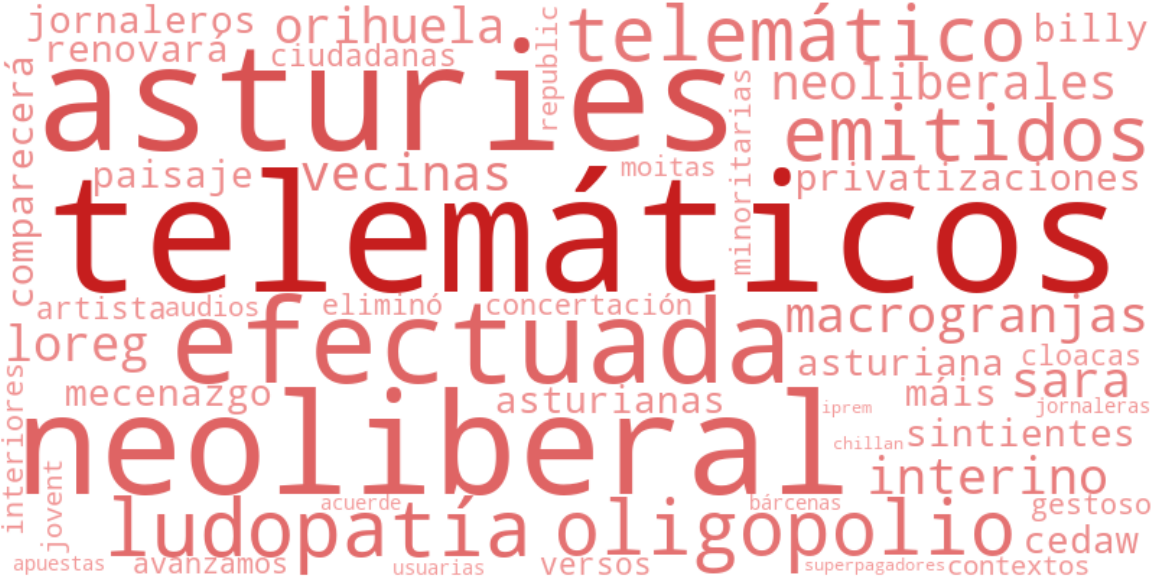
\includegraphics[width=\linewidth]{figures/congress_left.pdf}

		\end{minipage}
		\hspace{0.04\textwidth}
		\begin{minipage}{0.46\textwidth}
						\label{fig:worcloud2}
						\captionof{figure}{Word Cloud Top Right Words}
			\centering
			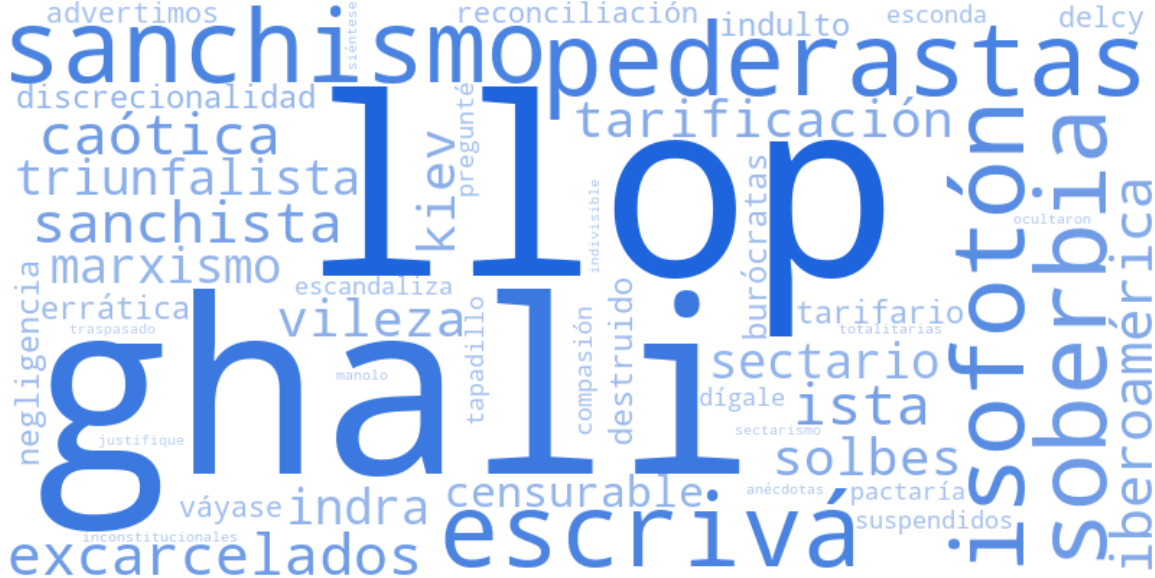
\includegraphics[width=\linewidth]{figures/congress_right.pdf}


		\end{minipage}
		\caption*{\small Notes: The wordclouds represent the Top Words with lowers (left) and highest (right) scores as defined in equation \ref{eq:log_ratio}. Size of the word is weighted by word frequency appearance.  }
	\end{figure}
	
	
	
	
	
	Finally, to classify the channel data, I calculate for each channel the fraction of tokens that appear in the left-coded list versus the right-coded list. This yields an index of ideological slant that reflects which side's language is more prevalent in the channel’s content. The 
	
	
	
	\begin{figure}[H]
		\centering
		\caption{Normalized Ideology Scores}
		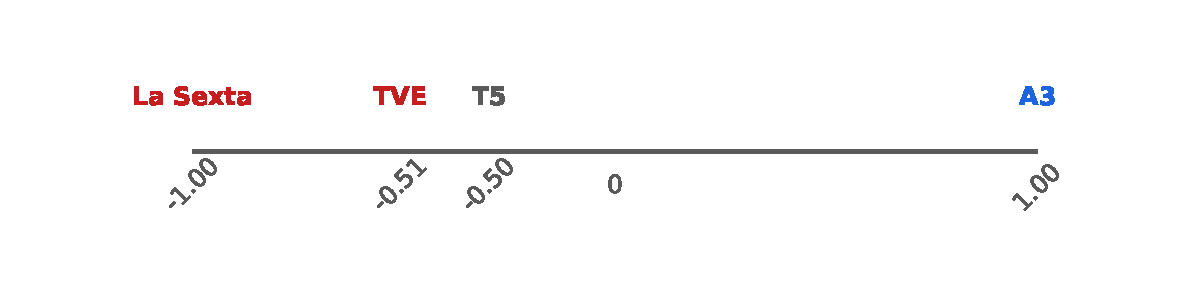
\includegraphics[width=120mm]{figures/congress_line}
		\caption*{\small Notes: The figure shows the normalized ideology positions of the channels after the text classification based on congress speeches. }
		\label{fig:congress_line}
	\end{figure}
	

	
	

	
	\begin{comment}
	
	\subsection{Alternative methods for segment splitting in unstructured text}
	
	I explain here different unsupervised text splitting methods that were tried to split the segments of the day. To the best of my knowledge, these methods have not been applied before and can be easily extended to any TV news set up. The advantage of these techniques is that they provide an unsupervised way to split unstructured text into stories that is precise up to the second level, thus overcoming the problem of the manually annotated labels which goes at the minute level. There is, however, computational or financial costs in some of them that impeded me to use them for the whole dataset.
	
	\textbf{Image recognition}
	
	Outlets typically segment their sections by means of captions where they introduce headers for the upcoming story. Exploiting our video dataset, I designed an unsupervised image recognition algorithm that tracks the appearance of those new segments and produces a set of times that serve as text splitters. Although precise, the disadvantage of this method is that it remains computationally intensive as videos need to be segmented and then processed into the algorithm. Computational cost can be reduced by focusing on the lower bottom of the screen  only (figure \ref{figure:image_rec}), which is the area where the output is expected to appear.
	
	\begin{figure}[H]
		\centering
		\caption{Example of  image story delimiter}
		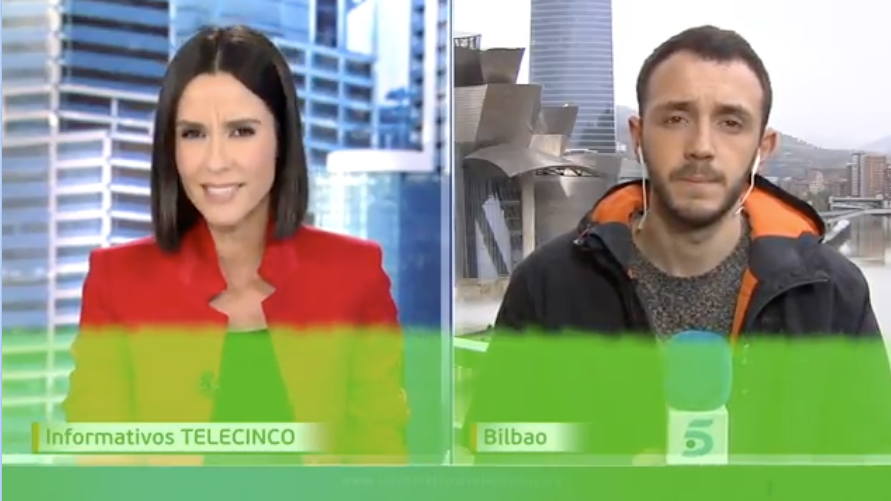
\includegraphics[width=100mm]{figures/image_recog}
		
		\caption*{\small Notes: Example of a image with a caption that delimits the beginning of a new section. The highlighted area shows the bottom of the image where image recognition can be applied to find such appearances.}
			\label{figure:image_rec}
	\end{figure} 
	
	
	
	
	\textbf{Speaker diarization}
	
	
	A less computationally expensive alternative consist on using \textit{speaker diarization} on the wav files. After transforming the mp4 file to audio using \textit{ffmpeg}, I use Google Cloud diarization tool to find the different speakers in an audio file. The most common (or most two common if it is a weekend) speakers overall corresponds to the presenter of the news. After allowing a flexible specification, one can identify break points by cheeking the seconds where the presenter comes back into scene making sure she is speaking long enough so that a new segment is being introduced. Figure \ref{fig:diarization} illustrates this procedure and the comparison with the manually annotated labels for an example day-channel.
	
	
	\begin{figure}[H]
		\centering
		\caption{Comparison audio splitting with annotated section splits}
		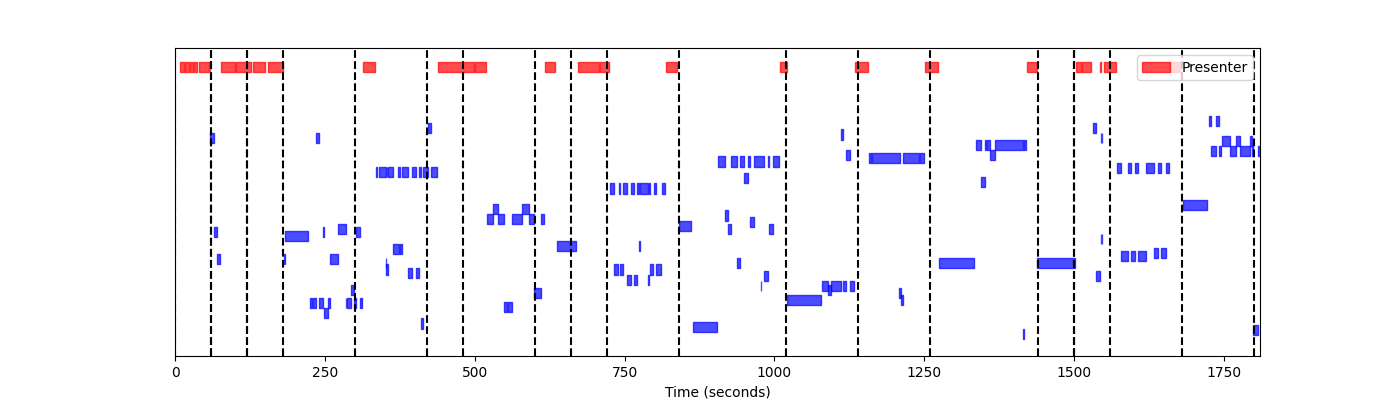
\includegraphics[width=120mm]{figures/speakers_all}
		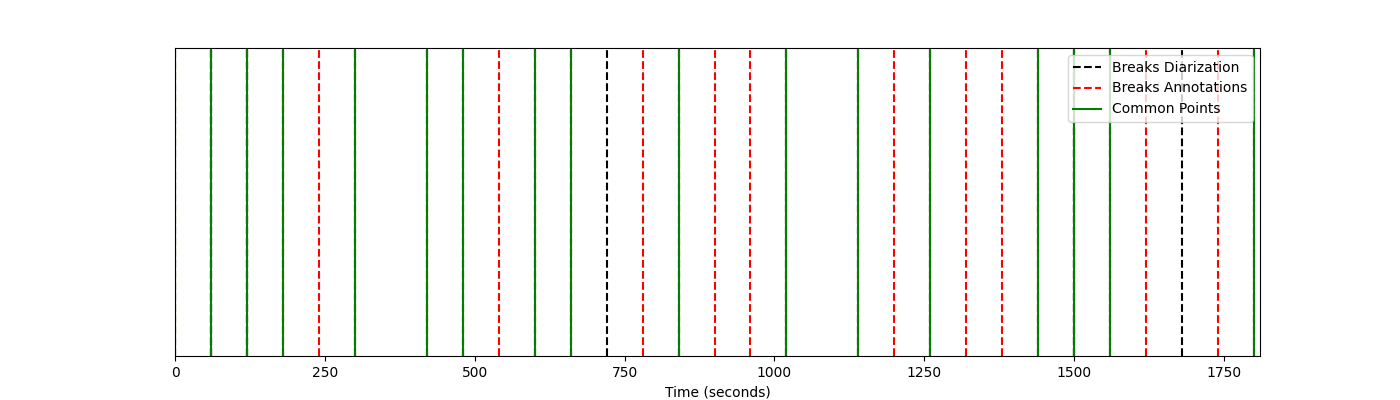
\includegraphics[width=120mm]{figures/speaker_timeline}
		\caption*{\small Notes: The top figure shows the timeline for the presenter audio (red) vs other audios recognized by \textit{speech2text} in a wav file for the 15th January 2023 in La Sexta. Vertical, black, dashed lines represent the predicted splits based on the diarization. The bottom figure combines these splits with the ones that come from the manually annotated figures. Red, dashed bars correspond to the breaks that come from the manually annotated GECA dataset. Green bars represent breaks where both the speaker diarization and the manual annotation coincide on a break. }
		\label{fig:diarization}
	\end{figure}
	
	
	
	
	\end{comment}
	
	
	
	
	
	
	
	
	
	
	

	
	
\end{document}